% Filename: latex_with_vim.tex
% This code is part of LaTeX with Vim.
% 
% Description: LaTeX with Vim is free book about Vim, LaTeX and Git.
% 
% Created: 29.03.12 11:18:28 PM
% Last Change: 29.03.12 11:21:52 PM
% 
% Author: Raniere Gaia Costa da Silva, r.gaia.cs@gmail.com
% Organization:  
% 
% Copyright (c) 2010, 2011, 2012, Raniere Gaia Costa da Silva. All rights 
% reserved.
% 
% This file is license under the terms of a Creative Commons Attribution 
% 3.0 Unported License, or (at your option) any later version. More details
% at <http://creativecommons.org/licenses/by/3.0/>.
\documentclass[12pt,a4paper,openright,twoside]{book}
\usepackage[brazil]{babel}
\usepackage[utf8]{inputenc}
\usepackage{pb-diagram}
\usepackage{graphicx, color}
\usepackage[top=3cm,left=2cm,right=2cm,bottom=3cm]{geometry}
\usepackage{subfig}
\usepackage{enumerate}
\usepackage{algorithmic}
\usepackage{algorithm}
\usepackage{listings}
\usepackage{listingsutf8}
\usepackage{indentfirst}
\usepackage{multirow}
\usepackage{amsthm}
\usepackage{amsmath}
\usepackage{amsfonts}
\usepackage{amssymb}
\usepackage{epsfig}
\usepackage{latexsym}
\usepackage{makeidx}
\usepackage{url}
\usepackage{hyperref}
\usepackage{breakurl}
\usepackage{multicol}
\usepackage{parcolumns}
\usepackage{empheq}
\usepackage[official]{eurosym}
\lstset{
breaklines=true,
literate={é}{{\'e}}1 {á}{{\'a}}1 {ã}{{\~a}}1,
}

% New commands and environment.
% Inline codes.
\newcommand{\lcode}[1]{\texttt{#1}}
% Display codes.
\lstnewenvironment{code}{ }{ }
\lstnewenvironment{latexcode}{ }{ }
% File codes.
\newcommand{\fcode}[1]{\lstinputlisting[frame=single,]{#1}}

\begin{document}
% Informations
\title{\LaTeX\ com Vim (e Git) \\ \vspace*{4pt} \small{Versão 1.0}}
\author{\url{https://github.com/r-gaia-cs/latex_with_vim/}}
\maketitle

% Frontmatter
\frontmatter 

% Filename: licence@latex_with_vim.tex
% This code is part of LaTeX with Vim.
% 
% Description: LaTeX with Vim is free book about Vim, LaTeX and Git.
% 
% Created: 29.03.12 11:16:53 PM
% Last Change: 29.03.12 11:28:44 PM
% 
% Author: Raniere Gaia Costa da Silva, r.gaia.cs@gmail.com
% Organization:  
% 
% Copyright (c) 2010, 2011, 2012, Raniere Gaia Costa da Silva. All rights 
% reserved.
% 
% This file is license under the terms of a Creative Commons Attribution 
% 3.0 Unported License, or (at your option) any later version. More details
% at <http://creativecommons.org/licenses/by/3.0/>.
\section*{Licen\c{c}a}

``\LaTeX\ no Vim'' de \url{http://code.google.com/p/latex-no-vim/} foi licenciada com uma Licen\c{c}a Creative Commons - Atribui\c{c}\~{a}o - Uso N\~{a}o Comercial 3.0 N\~{a}o Adaptada (\url{http://creativecommons.org/licenses/by-nc/3.0/}). 

Com base na obra dispon\'{i}vel em \url{https://github.com/r-gaia-cs/latex_with_vim}. 

Podem estar dispon\'{i}veis permiss\~{o}es adicionais ao \^{a}mbito desta licen\c{c}a em \url{https://github.com/r-gaia-cs/latex_with_vim}.

\begin{center}
    
\includegraphics[keepaspectratio=true]{../../figures/by_nc.png}
\end{center}

\section*{Licence}

``\LaTeX\ no Vim'' by \url{http://code.google.com/p/latex-no-vim/} is licensed under a Creative Commons Attribution 3.0 Unported License (\url{https://github.com/r-gaia-cs/latex_with_vim}).

Based on a work at \url{http://code.google.com/p/latex-no-vim/}.

Permissions beyond the scope of this license may be available at \url{https://github.com/r-gaia-cs/latex_with_vim}.

\begin{center}
    
\includegraphics[keepaspectratio=true]{../../figures/by_nc.png}
\end{center}


% Preface
% Filename: preface@latex_with_vim.tex
% This code is part of LaTeX with Vim.
% 
% Description: LaTeX with Vim is free book about Vim, LaTeX and Git.
% 
% Created: 29.03.12 11:52:59 PM
% Last Change: 29.03.12 11:53:32 PM
% 
% Author: Raniere Gaia Costa da Silva, r.gaia.cs@gmail.com
% Organization:  
% 
% Copyright (c) 2010, 2011, 2012, Raniere Gaia Costa da Silva. All rights 
% reserved.
% 
% This file is license under the terms of a Creative Commons Attribution 
% 3.0 Unported License, or (at your option) any later version. More details
% at <http://creativecommons.org/licenses/by/3.0/>.
\chapter*{Prefácio}
\addcontentsline{toc}{chapter}{Prefácio}

Meu primeiro contato com o Latex foi no primeiro ano de faculdade. Na época, me foi passado alguns tutoriais sobre Latex os quais considerei muito aquém do desejado.

Nos dois primeiros anos de faculdade, fui guardando algumas dicas úteis para trabalhar com o Latex. No segundo ano de faculdade tomei conhecimento do editor de textos Vim e logo em seguida do LaTeX-Suite, desenvolvido para o mesmo, que me facilitou muito trabalhar com o LaTeX. Aqui apresento algumas dicas do LaTeX e Vim que fui guardando nestes breves dois anos.

%No segundo ano de faculdade, tomei conhecimento do editor de texto VIM, que possui um conjunto de macros, dos quais gostei muito e por isso dou algumas dicas de como utilizá-lo também.

Na primeira parte aboraderemos o LaTeX e na segunda o Vim juntamente com o LaTeX-Suite.

Encontrar uma boa maneira de apresentar os comandos, ambientes e dicas do LaTeX foi uma tarefa difícil. Optou-se por começar preparando o sistema operacional para trabalhar com o LaTeX e em seguida como trabalhar com vários arquivos.

No capítulo \ref{sch:latex:preamble} abordamos o preâmbulo e no capítulo seguinte conhecimentos básicos para escrever uma carta. Outras ferramentas do LaTeX são apresentadas nos capítulos  \ref{css:latex:text_basic} e \ref{css:latex:text_basic} enquanto que no capítulo \ref{sch:latex:publi} abordamos comandos para a produção de teses e livros.

Informações sobre o modo matemático encontram-se nos capítulos \ref{sch:latex:math1}, \ref{sch:latex:math2}, \ref{sch:latex:math3} e \ref{sch:latex:math4}. No primeiro encontram-se os comandos básicos enquanto que no segundo apresentamos tabelas outros comandos. Os dois outros capítulos apresentam dicas para que as expressões matemáticas sejam apresentadas de maneira esteticamente melhor.

Depois de abordarmos o modo matemático temos os capítulos referentes a tabelas, figuras, códigos, algorítmos e bibliografia.

Já na segunda parte, abordamos nos três primeiros capítulos o Vim e nas duas últimas o LaTeX-Suite.

\subsection*{Agradecimentos}
Meus agradecimentos a todos que me motivaram a este trabalho e com ele contribuíram. Um muito obrigado para Marina Lima Morais pelo apoio na revisão do trabalho.
 

\tableofcontents 
\listoftables

% Mainmatter
\mainmatter 

\part{Introdu\c{c}\~{a}o}
% Vim
% Filename: p1_vim@latex_with_vim.tex
% This code is part of LaTeX with Vim.
% 
% Description: LaTeX with Vim is free book about Vim, LaTeX and Git.
% 
% Created: 29.03.12 11:30:17 PM
% Last Change: 29.03.12 11:30:24 PM
% 
% Author: Raniere Gaia Costa da Silva, r.gaia.cs@gmail.com
% Organization:  
% 
% Copyright (c) 2010, 2011, 2012, Raniere Gaia Costa da Silva. All rights 
% reserved.
% 
% This file is license under the terms of a Creative Commons Attribution 
% 3.0 Unported License, or (at your option) any later version. More details
% at <http://creativecommons.org/licenses/by/3.0/>.
\chapter{Vim}
O texto a seguir foi adaptado da Wikipedia (\url{http://en.wikipedia.org/wiki/Vim_(text_editor)}).

Vim é um editor de texto originalmente desenvolvido por Bram Moolenaar em 1991, para Amiga computer. O nome Vim é um acrónimo para ``Vi IMproved'', porque o Vim foi criado como uma extensão do vi editor, com ferramentas adicionais para auxiliar na edição de códigos fontes.

Embora Vim tenha sido originalmente lançado para Amiga, atualmente é desenvolvido para se multi-plataforma, suportanto muitas outras plataformas.

Vim é livre e open source software, e sua licença é compatível com GNU General Public License.


% LaTeX
% Filename: p1_latex@latex_with_vim.tex
% This code is part of LaTeX with Vim.
% 
% Description: LaTeX with Vim is free book about Vim, LaTeX and Git.
% 
% Created: 29.03.12 11:29:58 PM
% Last Change: 29.03.12 11:30:10 PM
% 
% Author: Raniere Gaia Costa da Silva, r.gaia.cs@gmail.com
% Organization:  
% 
% Copyright (c) 2010, 2011, 2012, Raniere Gaia Costa da Silva. All rights 
% reserved.
% 
% This file is license under the terms of a Creative Commons Attribution 
% 3.0 Unported License, or (at your option) any later version. More details
% at <http://creativecommons.org/licenses/by/3.0/>.
\chapter{\LaTeX}
O texto a seguir foi adaptado da Wikipedia (\url{http://en.wikipedia.org/wiki/TeX}).

\TeX\ ou TeX é um sistema de tipografia desenvolvido e em sua maior parte escrita por Donald Knuth. Foi desenvolvido com dois objetivos principais em mente: permitir qualquer pessoa produzir livros de alta qualidade usando uma quantidade razoável de esforço, e providenciar um sistema que produza exatamente o mesmo resultado em todo computador, hoje e no futuro.

TeX é um meio popular para tipografia de fórmulas matemáticas complexas.

O texto a seguir foi adaptado da Wikipedia (\url{http://en.wikipedia.org/wiki/LaTeX}).

\LaTeX\ ou LaTeX é uma linguagem de marcação e preparativo do sistema para o TeX. O termo LaTeX refere-se apenas a linguagem na qual o documento é escrita. Para a criação de um documento em LaTeX, um arquivo com a extensão \textsf{.tex} deve ser criado utilizando algum editor de texto.

LaTeX tenta prover uma linguagem de alto nível, para acessar o poder do TeX. LaTeX essencialmente comprime uma coleção de macros originais do TeX e um programa para processar o documento LaTeX. Devido aos comandos TeX serem de baixo nível é usualmente mais simples para o usuário final utilizar o LaTeX.

LaTeX foi originalmente escrito por Leslie Lamport e tornou-se o método dominante para uso do TeX.

Atualmente, o Latex encontra-se na versão \LaTeXe\ ou LaTeX2e e é distribuido de acordo com os termos do LaTeX Project Public License (LPPL), sendo um software livre.


% Git
% Filename: p1_git@latex_with_vim.tex
% This code is part of LaTeX with Vim.
% 
% Description: LaTeX with Vim is free book about Vim, LaTeX and Git.
% 
% Created: 29.03.12 11:29:02 PM
% Last Change: 29.03.12 11:29:45 PM
% 
% Author: Raniere Gaia Costa da Silva, r.gaia.cs@gmail.com
% Organization:  
% 
% Copyright (c) 2010, 2011, 2012, Raniere Gaia Costa da Silva. All rights 
% reserved.
% 
% This file is license under the terms of a Creative Commons Attribution 
% 3.0 Unported License, or (at your option) any later version. More details
% at <http://creativecommons.org/licenses/by/3.0/>.
\chapter{Git}
Alguns artigos muito interessantes s\~{a}o:
\begin{enumerate}
    \item \url{http://www.dribin.org/dave/blog/archives/2007/12/28/dvcs/}
        \begin{quote}
            Choosing a Distributed Version Control System
            By Dave on December 28, 2007 4:17 PM | Permalink
            Version control systems. If you’re a software developer, you’re (hopefully) using one. The most popular version control system (VCS) is no doubt Subversion. It’s what I currently use on every one of my projects, both personal and business. While Subversion is a great improvement over previous VCSs I’ve used (CVS, RCS, SCCS, ClearCase and home grown), it’s not without its warts. And unless you’ve been living under a rock, it’s starting to get some serious competition. I’ve decided to play the field and see what this competition has to offer.

            The Rise of Distributed Version Control Systems

            Within the last year, distributed version control systems (DVCSs) have really started to break into mainstream development. DVCSs are a different way of thinking about version control. They break the mold of a single, central repository that most VCSs have, like Subversion and CVS. A distributed VCS is different. Each user checks out their own full copy of the repository and commit locally to it. These changes may then be shared with others, often by syncing to a canonical repository.

            I’m not going to talk much about how DVCSs work or the benefits of a distributed VCS versus a central VCS. That has already been much discussed elsewhere. I highly recommend watching Linus Torvalds’ YouTube video on Git and reading Wincent Colaiuta’s piece called Why Distributed Version Control.

            The Options

            My own personal desire came when I was without Internet access for a few days (shocking, I know), and realized that offline commits would be really useful. Also, I’ve many times thought it would be nice to be able to do local commits during a large feature. DVCSs solve both of these issues cleanly and elegantly. Commit to your local repository, and push out the changes when you have an Internet connection or when you’re confident the feature is stable enough.

            So now that I’d bought into DVCS hype, I decided it was time to kick the tires and try them out. As a new user, I’ve found that choosing a DVCS is a bit overwhelming. The number of DVCSs to choose from is staggering: Git, Mercurial, Bazaar, darcs, Monotone, Codeville, arch. The big three I decided to look at are Git, Mercurial, and Bazaar. After spending a day look these, I’m still not fully decided, but here are my thoughts so far.

            What’s Wrong with Subversion

            Before going into the details, let me first cover what I think is wrong with Subversion. Subversion is a great step up from CVS, but here’s what bothers me:

            The whole trunk/tags/branches convention
            No offline commits
            .svn files everywhere
            svn:external is weak
            I understand that copies are a cheap operation in Subversion, but that’s an implementation detail. Tags should be immutable. No, I’ve never accidentally checked out a branch and committed to one. But still, if it’s a convention and “best practice” to use trunk/tags/branches, Subversion should have the concept of a “project” built in. If a theoretical svn tag is implemented as a copy under the hood, then so be it. That’s an implementation detail.

            Instead of svn:external, I use Piston. This makes it easy to lock an external to a tag, and then switch tags as you change versions. It works pretty well, if not a bit slow.

            You’ll notice I don’t even mention branching and merging. I’ve never used it, mainly because I haven’t felt the need. Also, because it’s hard. Repeated merges from a branch are painful. This is one area that Linus harps on. He claims that maybe if Subversion branching and merging didn’t suck so much, people would actually use them. Quite possible, but as of now, it’s not something that bothers me.

            Git

            Git is the DVCS being used for Linux kernel development. It was started by Linus himself after the whole BitKeeper Debacle of ‘05. While it started off as very user-unfriendly, and something only Linus could love, in the last year it has grown much better. It has since gained a lot of traction and is arguably the most popular system.

            The Mac blogosphere has been a buzz with developers switching or looking into Git over the last six months. Wincent Colaiuta has been actively blogging about his use of Git since his switch to July. Michael Tsai also switched to Git around July. Fraser Speirs has a couple posts about being intrigued by Git (1, 2). Bill Bumgarner claims Git will eat Subversion’s Lunch (though he’s really talking about DVCS eating Subversion’s lunch). Steve Dekorte switched to Git, after using darcs for a bit. Drew McCormack started using Git earlier this month.

            I’ve also seen quite a few Ruby on Rails blogs talk about using Git, as well, so to me it’s the front-runner. Here’s my evaluation:

            Pros:

            Single top-level .git file
            Mature
            Most common DVCS
            Decent documentation
            Used by a large project (Linux kernel)
            Easy to compile
            Submodule support via git submodule
            Can be shared read-only via static files over HTTP
            Tracks content, not files
            Cons:

            Advanced branch features are not something I’d really use
            Spews 146 files into my PATH:

% ls /usr/local/bin/git* | wc -l
            146
            Poor Windows support

            Directories are not versionable
            Submodule support feels awkward. “Deliberately” minimal. Can’t lock to a specific tag?
            Read-only static HTTP setup is a bit obtuse (--bare and update-server-info)
            Tracks content, not files (yes, it’s both a pro and a con)
            The hundreds of files in PATH is more of an annoyance than a real criticism, and it’s going to be fixed. As of version 1.5.4, the dashed form of commands (e.g. git-commit) is deprecated. Version 1.6.0 plans on moving the dashed support files out of PATH.

            The biggest weakness for me is the poor Windows support. While I’m not currently working on any Windows projects, I’ve had client projects in the past that are either cross platform or use Windows as their development platform. If I’m going to be going through the trouble of learning a new version control system, it makes sense to learn something I can take with me on any project.

            I’m also unsure of “tracks content, not files”. This means that Git can theoretically track a function moved from one file to another. Wincent praises Linus as a “frickin’ genius” because of this. Most likely Wincent is correct, but my little mind has problems giving up on the versioning of files.

            Mercurial

            Git isn’t getting all the love. Mercurial, sometimes known as “hg” (as Hg is the chemical symbol for mercury), was also started due to the BitKeeper Debacle of ‘05. It has since been embraced by large projects like OpenSolaris, OpenJDK, NetBeans, and Mozilla. Linus himself even praises Mercurial as the only other DVCS worthy as competition to Git. Here’s my evaluation:

            Pros:

            Single top-level .hg file
            Used by large projects (OpenSolaris, OpenJDK, NetBeans, Mozilla)
            Command usage is more similar to Subversion
            Cross platform to Windows
            Submodule support via the Forest extension
            Simpler branch model (a clone is a branch)
            IDE integration with Eclipse and NetBeans
            TortoiseHG in the works
            Excellent documentation
            Can be shared read-only via static files over HTTP
            Cons:

            The use of hgmerge seems a little wonky
            Still pre-1.0 (currently 0.9.5)
            Forest extension is poorly documented
            Static HTTP sharing is self-described as “much slower, less reliable”
            Requires a CGI script for practical sharing over HTTP
            Directories are not versionable
            Tags are stored in .hgtags
            The .hgtags file is a plain old text file that is versioned along with everything else. Because it’s not special in any way, it needs merging and can even get conflicts. This is probably not an issue in practice (sort of like Subversion’s use of tags), but it still seems wonky.

            The hgmerge script handles merges, and there’s no standard way to say “this is a binary file, don’t merge it”. There’s more on the Wiki about this. Again, probably not a problem in practice, but it, too, seems wonky.

            Probably the main weakness for me is that it’s less common than Git. I imagine Sun’s new usage of Mercurial will be changing that. Many in the Java community will probably follow. Also, for some reason, Subversion developers don’t hate Mercurial like they hate Git, either. Perhaps that has more to do with Linus calling Subversion developers “stupid” and telling them they should be locked up in a mental institution than basis in fact, though.

            Bazaar

            Bazaar, sometimes known as bzr, is a DVCS used by Ubununtu and funded by the same company, Mark Shuttleworth’s Canonical Ltd.

            Pros:

            Single top-level .bzr file
            Directories are versionable
            Recently hit 1.0 (December 14, 2007)
            Excellent documentation
            Fast (bad performance during OpenSolaris investigation has supposedly been fixed)
            Cross platform to Windows
            Merge architecture seems more sane than Mercurial
            Can be served up read-only by static HTTP
            Simpler branch model (a clone is a branch)
            Cons:

            No submodule support
            Has been a minor pain to install on Mac OS X 10.5 and Centos 5.1
            Not really used by large projects outside of Ubuntu
            bzrweb is not as advanced as Git/Mercurial counterpart
            Sharing over static HTTP is slow
            A faster smart server is a major focus of the next version
            Historically, the main complaint about Bazaar has been it’s performance. In fact, the main reason why OpenSolaris dismissed Bazaar was due to poor performance. But that eval was a year ago, which is essentially an eternity. Since then, Bazaar has hit 1.0 and those performance criticisms have supposedly been addressed.

            Also, Bazaar has a history of changing the repository format. Again, now that Bazaar has hit 1.0, hopefully they won’t be doing this very often, any more.

            The main weakness of Bazaar for me is that it’s even less popular than Mercurial. There’s something to be said about using a tool that other people know, especially when the whole point of a DVCS is to get collaboration.

            Then again, the directory support is intriguing, and I do like the ability to publish repositories using without a CGI script. Also, as dbt said on Twitter:

            [T]he general opinion I’ve had is that bzr went for correctness before speed, while hg went the other way.

            The Golden Age of Version Control Systems

            Confused yet? I know I am. There really is no run-away winner for me. While I could probably use any one of these and be happier than using Subversion, I keep teetering between Git and Mercurial. Which is more appealing, Git’s content tracking or Mercurial’s Windows support? Maybe I’ll toss a coin. Update: I’ve chosen Mercurial.

            If I were more patient, I’d wait a year. The year of 2007 is looking to be the beginning of the Golden Age of Version Control Systems. The DVCs became more stable and got much better documentation. Over the next year, I think we’ll see a lot of activity in the VCS area. If the progress of Git, Mercurial, and Bazaar in the last twelve months is any indication, they’ll be even further ahead of Subversion in another twelve months.

            Even the Subversion team is being forced to take notice, albeit a bit defensively at times. Subversion 1.5 is going to bring better merge support. Future versions may even have local commits and stop spewing .svn files everywhere. Unfortunately, by the time Subversion gets these features, the DVCS guys will have had plenty of time to spit and polish their offerings, too.

            All in all, this competition is good for you and me, the end users of VCSs. I’m really excited to see where the DVCSs are in another year. In the meantime, I also want to be an early adopter.

            Corrections 31-Dec-2007: I added some info about Mercurial’s static-http and more info on Bazaar’s sharing over HTTP and smart server.
        \end{quote}
    \item \url{http://www.smashingmagazine.com/2008/09/18/the-top-7-open-source-version-control-systems/}
\end{enumerate}


\part{Vim}
% Introdução
% Filename: p2_basic_of_vim@latex_with_vim.tex
% This code is part of LaTeX with Vim.
% 
% Description: LaTeX with Vim is free book about Vim, LaTeX and Git.
% 
% Created: 29.03.12 11:31:01 PM
% Last Change: 29.03.12 11:56:53 PM
% 
% Author: Raniere Gaia Costa da Silva, r.gaia.cs@gmail.com
% Organization:  
% 
% Copyright (c) 2010, 2011, 2012, Raniere Gaia Costa da Silva. All rights 
% reserved.
% 
% This file is license under the terms of a Creative Commons Attribution 
% 3.0 Unported License, or (at your option) any later version. More details
% at <http://creativecommons.org/licenses/by/3.0/>.
\chapter{Introdução} \label{sch:vim:basic}
O Vim acompanha a grande maioria das distribuições Linux e também está disponível para o Windows. Na Figura \ref{fig:vim_screen} encontramos a tela incial do Vim.
\begin{figure}[h!]
    \centering
    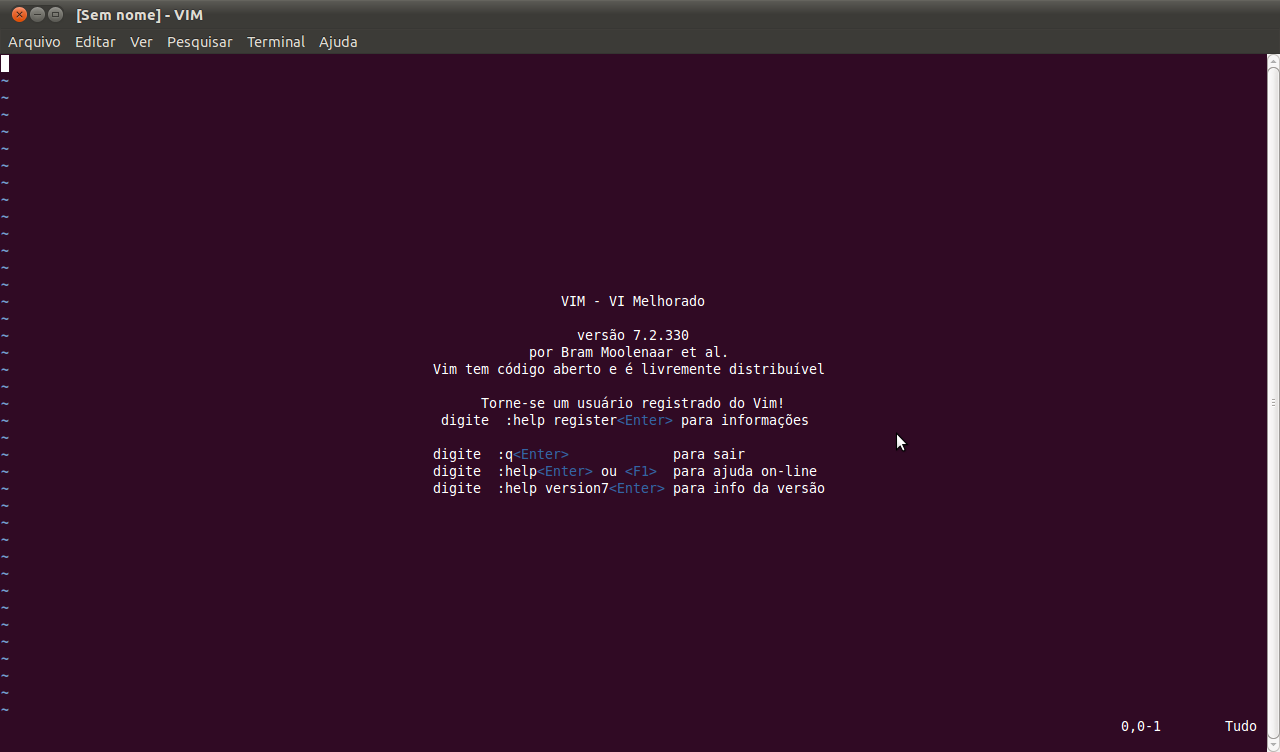
\includegraphics[height=6cm]{figures/vim_screen}
    \caption{Tela inicial do Vim.}
    \label{fig:vim_screen}
\end{figure}

O GVim é uma implemantação do Vim com interface gráfica e na Figura \ref{fig:gvim_screen} encontramos a tela incial do mesmo.
\begin{figure}[h!]
    \centering
    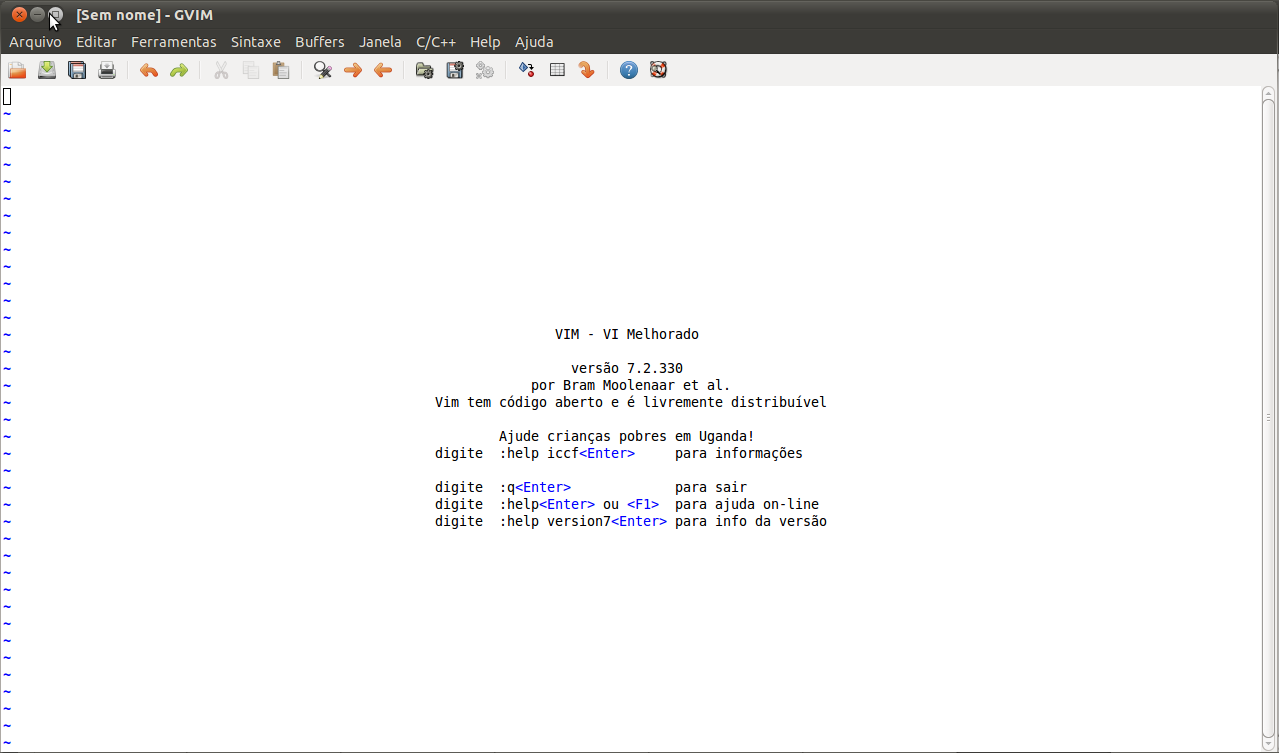
\includegraphics[height=6cm]{figures/gvim_screen}
    \caption{Tela inicial do GVim.}
    \label{fig:gvim_screen}
\end{figure}

\section{Instalação}
\subsection{Windows}

Para a instalação no Windows, versões a partir do XP, pode-se baixar o arquivo disponível em \url{ftp://ftp.vim.org/pub/vim/pc/gvim73_46.exe} e executá-lo.

Destaca-se que uma versão portátil do GVim é encontrada em: \url{http://portablegvim.sourceforge.net/}

\subsection{Linux}

A instalação da distribuição no Ubuntu pode ser feita via terminal com o seguinte comando:
\begin{code}
    sudo apt-get install vim
\end{code}

\section{Iniciando o Vim}

Para iniciar o Vim podemos, a partir da \textit{shell}\footnote{Correspode ao ``prompt de comando'' do usuário}, utiliza-se o comando
\begin{code}
    vim
\end{code}
iniciando o Vim com a tela de boas-vindas ou o comando
\begin{code}
    vim XXX
\end{code}
iniciando o Vim e abrindo o arquivo de texto \lcode{XXX}.

\section{Modos}

No Vim lidamos com dois modos operacionais:
\begin{enumerate}
    \item \textit{Modo de comando};
    \item \textit{Modo de entrada}.
\end{enumerate}

O Vim é iniciado por padrão no \textit{modo de comando} onde cada tecla, ou combinação delas, realizar algum comando. Para alguns comandos precisa-se digitar \lcode{:} , dois pontos, de modo que o cursor muda para o última linha da janela, como apresentado na Figura \ref{fig:vim_colon_screen}. Para que o cursor saia da última linha da janela deve-se precionar a tecla \lcode{Enter}.
\begin{figure}[h!]
    \centering
    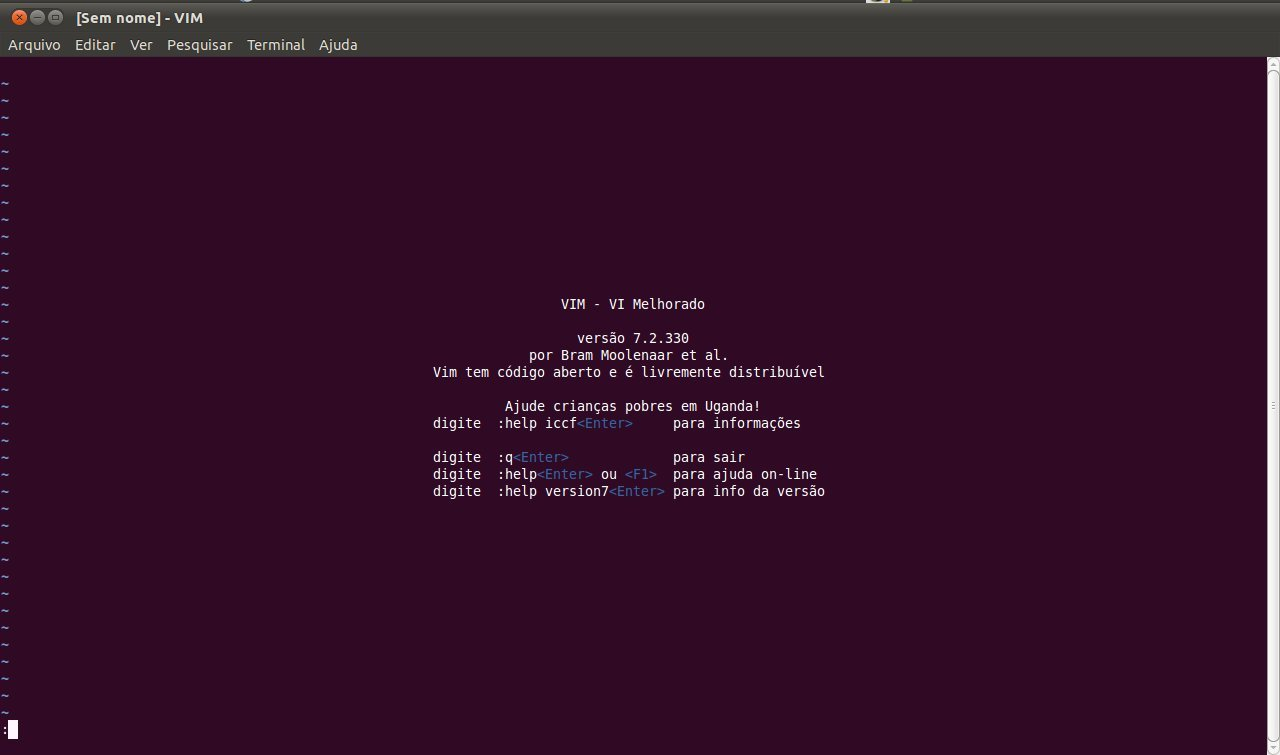
\includegraphics[height=6cm]{figures/vim_colon_screen}
    \caption{Cursor na última linha da janela.}
    \label{fig:vim_colon_screen}
\end{figure}

Já no \textit{modo de entrada}, cada tecla corresponde a uma caractere e é indicado pela presença do texto \lcode{- - INSERÇÃO - -} na última linha da janela, como podemos observar na Figura \ref{fig:vim_insert_screen}.
\begin{figure}[h!]
    \centering
    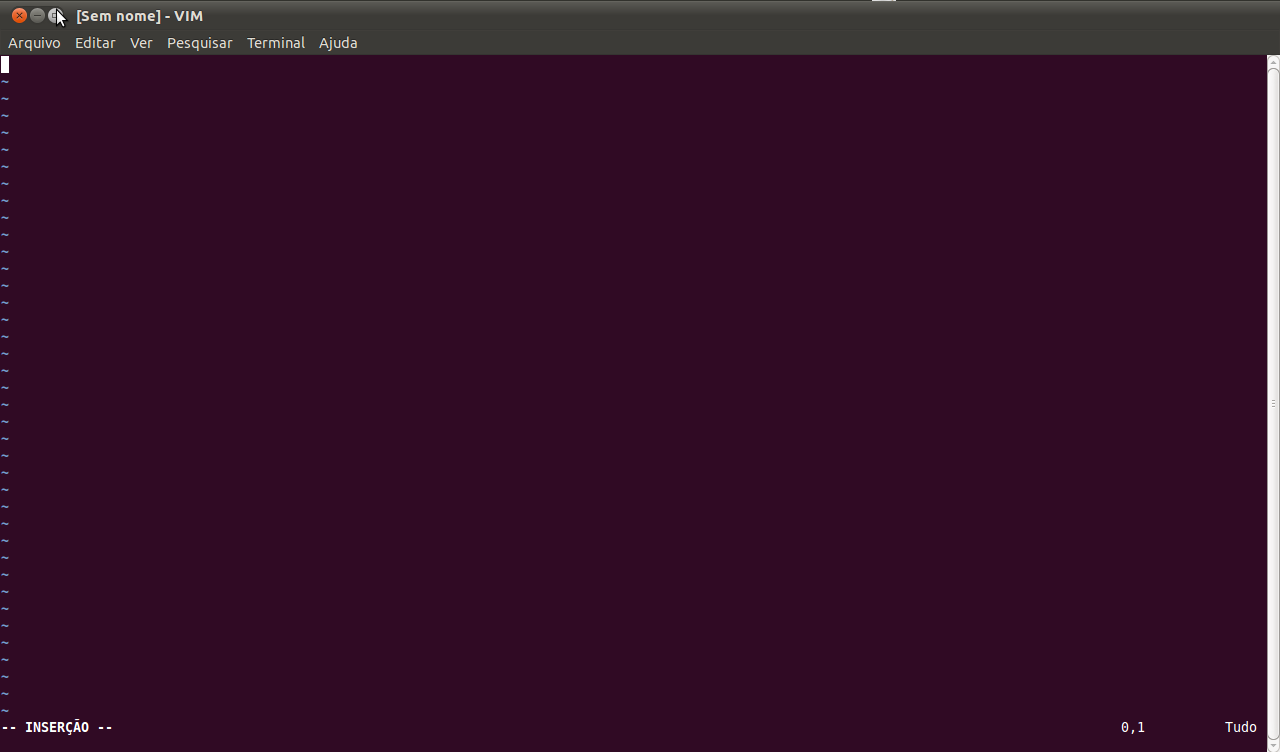
\includegraphics[height=6cm]{figures/vim_insert_screen}
    \caption{Vim no \lcode{modo de entrada}.}
    \label{fig:vim_insert_screen}
\end{figure}
Para mudar do \textit{modo de comando} para o \textit{modo de entrada} deve-se pressionar a tecla \lcode{i} e para retornar a tecla \lcode{Esc}.

Na Figura \ref{fig:vim_modes} observamos como os modos estão relacionados.
\begin{figure}[h!]
    \centering
    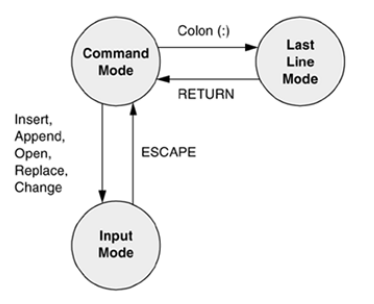
\includegraphics[height=6cm]{figures/vim_modes}
    Fonte: \cite{Sobell:2005:PracticalGuide}
    \caption{Esquema dos modos operacionais do Vim.}
    \label{fig:vim_modes}
\end{figure}

\section{Abrindo um arquivo}
Para abrir um arquivo para edição utiliza-se o comando \lcode{:e} seguido do nome do arquivo a ser editado. Em alguns casos pode ser necessário utilizar o comando \lcode{:e!} ao invés do \lcode{:e} .

\section{Salvando o arquivo}
Para salvar o arquivo atual utiliza-se o comando \lcode{:w}. Em alguns casos pode ser necessário utilizar o comando \lcode{:w!} ao invés do \lcode{:w} .

Caso deseje-se salvar o arquivo atual sem sobrescrever o arquivo existente pode-se utilizar o mesmo comando seguido pelo nome do novo arquivo. 

\section{Fechando o Vim}
Para fechar o Vim deve-se utilizar o comando \lcode{:q} ou \lcode{:q!} para fechar o Vim ignorando as alteração efetuadas no arquivo.

\section{Configuração}

A configuração padrão do Vim, ao ser inicializado, pode ser alterada ao modificar o arquivo \lcode{vimrc}. Nas distribuições Linux deve-se procurar na pasta de usuário pelo arquivo \lcode{.vimrc}, enquanto que no Windows por \lcode{\_vimrc}.

Quando o arquivo \lcode{vimrc} contendo as linhas do código abaixo
\begin{code}
    "Habilita highlight
    syntax on
    "Habilita uso de plugin's dependendo do tipo do arquivo
    filetype plugin on
    "Habilita identacao de acordo com o tipo do arquivo
    filetype indent on
    "Mostra no inicio de cada linha o numero da mesma
    set number
\end{code}
promove o descrito nas linhas iniciadas com aspas\footnote{Nos arquivos utilizados pelo Vim, linhas iniciadas por aspas são comentários e por isso ignoradas pelo Vim.}.

Para outras configurações sugere-se olhar os seguintes endereços:
\begin{itemize}
    \item \url{http://aurelio.net/doc/dotfiles/vimrc.txt}
    \item \url{http://aurelio.net/vim/vimrc-voyeg3r.txt}
    \item \url{http://aurelio.net/vim/vimrc-ivan.txt}
\end{itemize}

\section{Ajuda}

A ajuda no Vim pode ser obtida pelo comando \lcode{:help} .


% Primeiros comandos
% Filename: p2_start_with_vim@latex_with_vim.tex
% This code is part of LaTeX with Vim.
% 
% Description: LaTeX with Vim is free book about Vim, LaTeX and Git.
% 
% Created: 29.03.12 11:31:41 PM
% Last Change: 30.03.12 12:02:00 AM
% 
% Author: Raniere Gaia Costa da Silva, r.gaia.cs@gmail.com
% Organization:  
% 
% Copyright (c) 2010, 2011, 2012, Raniere Gaia Costa da Silva. All rights 
% reserved.
% 
% This file is license under the terms of a Creative Commons Attribution 
% 3.0 Unported License, or (at your option) any later version. More details
% at <http://creativecommons.org/licenses/by/3.0/>.
\chapter{Primeiros comandos} \label{sch:vim:start}
\section{Movimentando o cursor e saltos}
No \textit{modo de comando} a movimentação do cursor pode ser realizada pelas setas direcionais ou pelas teclas \lcode{h}, \lcode{j}, \lcode{k} e \lcode{l} que correspondem, respectivamente, a esquerda, abaixo, encima e direita.

Já no \textit{modo de entrada} a movimentação só pode ser feita pelas setas direcionais.

\subsection{Caracteres}
Pode-se realizar saltos ao movimentar o cursor em uma mesma linha e para isso deve-se digitar quantos caracteres devem ser saltados e em seguida a direção a ser tomada. Por exemplo, comando \lcode{8l} salta $8$ caracteres a direita e \lcode{20h} $20$ caracteres a esquerda.

\subsection{Palavras}
O comando \lcode{w} leva o cursor para a próxima palavra e \lcode{W} para a próxima precedida por um espaço.

O comando \lcode{b} leva o cursor para a palavra anterior e \lcode{B} para a anterior precedida por um espaço.

Já o comando \lcode{e} leva o cursor para o fim da palavra e \lcode{E} para o fim da próxima palavra precedida por um espaço.

\subsection{Sentenças e Parágrafos}
O comando \lcode{)} leva o cursor para a próxima sentença e \lcode{\}} para o próximo parágrafo.

Já o comando \lcode{(} leva o cursor para a sentença anterior e \lcode{\{} para o parágrafo anterior.

\subsection{Linha}
O comando \lcode{0} promove o cursor para o início da linha e \$ para o final.

Já comando \lcode{Enter} leva o cursor para a linha seguinte e \lcode{-} para a linha anterior.

É importante saber a diferença entre os comandos \lcode{j} e \lcode{Enter}. O comando \lcode{j} leva o cursor para a próxima linha mantendo a mesma coluna enquanto o comando \lcode{Enter} para o início da próxima linha. A diferença entre os comandos \lcode{k} e \lcode{-} é semelhante ao apresentado pelos comandos \lcode{j} e \lcode{Enter}.

Para pular diretamente para a quinta linha do documento pode-se utilizar o comando \lcode{:$5$} e de maneira análoga para qualquer outra linha.

\subsection{Tela}
No \textit{modo de comando} pode-se posicionar cursor em relação a janela. Para isso deve-se utilizar os comandos \lcode{H}, primeira linha da janela, \lcode{M}, meio da janela,  e \lcode{L}, última linha da janela.

\section{Busca}
O comando \lcode{f} seguido de um caractere busa a primeira ocorrência do mesmo a direita da atual posição do cursor e \lcode{F} a próxima ocorrência a esquerda. Por exemplo, para ir a próxima ocorrência da letra \lcode{a} deve-se utilizar o comando \lcode{fa} e para a ocorrência anterior da letra b \lcode{Fb}.

O comando \lcode{;} repete a busca.

Já o comando \lcode{/} e \lcode{?} seguido por uma string e finalizado por \lcode{Enter} efetuam a busca pela primeira ocorrência da string após o cursor e antes do mesmo, respectivamente. No caso de os caracteres \lcode{/} e \lcode{?} aparecerem na string eles devem ser precedidos por \textbackslash.

Para repetir a busca pode-se utilizar o comando \lcode{n}. Já o comando \lcode{N} realiza a busca no sentido contrário.

Destaca-se que o comando \lcode{/} ou \lcode{?} leva o cursor para última linha da janela como ilustrado na Figura \ref{fig:vim_search_screen}.
\begin{figure}[h!]
    \centering
    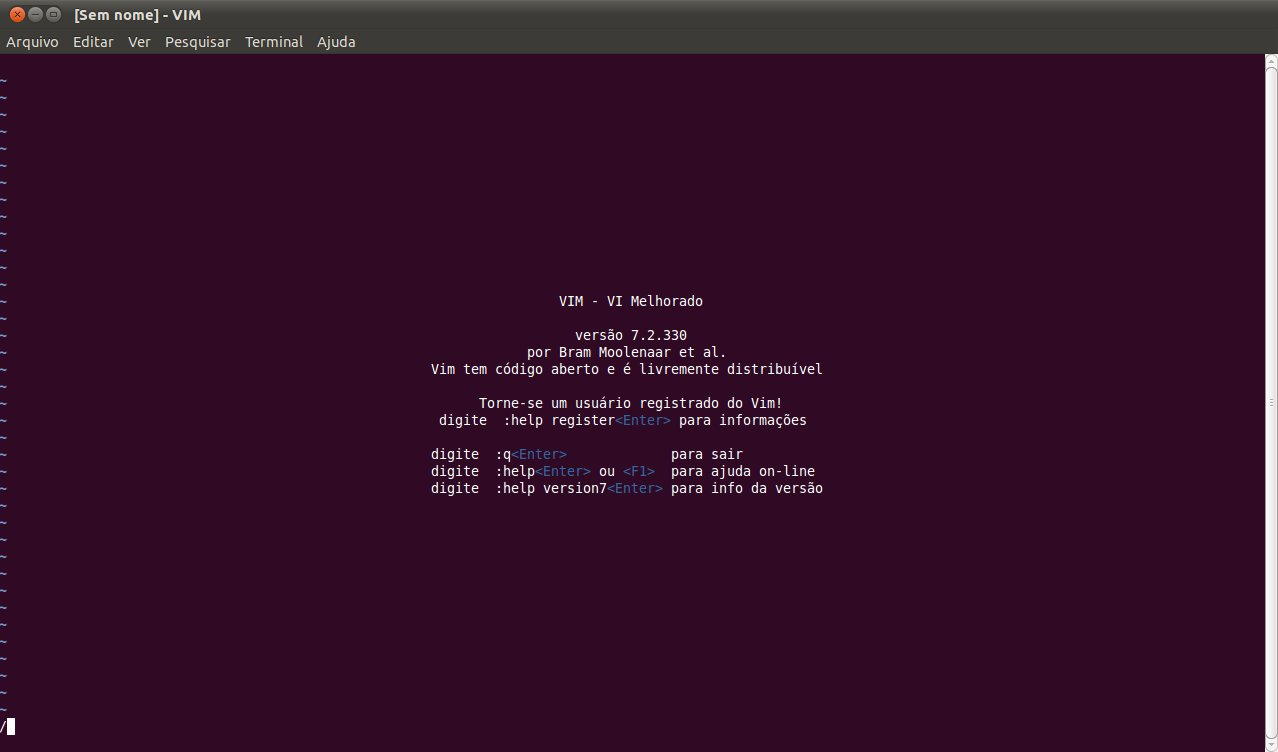
\includegraphics[height=6cm]{figures/vim_search_screen}
    \caption{Tela referente a busca.}
    \label{fig:vim_search_screen}
\end{figure}

Para localizar o par de um parênteses, colchetes ou chaves deve-se utilizar o comando \% quando o cursor estiver sobre um destes.

\section{Editando um texto}
\subsection{Linhas}
O comando \lcode{o} inicia uma nova linha abaixo da linha atual e iniciar o \textit{modo de edição} com o cursor posicionado na nova linha. Já \lcode{O} funciona de maneira semelhante ao \lcode{o} mas iniciando uma nova linha acima da linha atual.

O comando \lcode{J} junta a próxima linha a atual.

\subsection{Deletando}
Deve-se utilizar os comandos \lcode{x}, para apagar um único caractere, \lcode{dw}, para apagar uma palavra, e \lcode{dd}, para apagar uma linha.

O comando \lcode{X} apaga o primeiro caractere a esquerda do cursor.

É permitido utilizar um número antes do comando de forma que \lcode{6x} apaga 6 caracteres,  \lcode{3dw} apaga duas palavras e \lcode{2dd} apaga duas linhas.

O comando \lcode{d}\$ apaga do cursor ao fim da linha e \lcode{d}\textasciicircum apaga do cursor ao inicio da linha.

No \textit{modo de entrada} pode-se utilizar a tecla \lcode{Backspace} para apagar um único caractere.

O comando \lcode{Ctrl-w} suprimi o texto anterior ao cursor até o primeiro espaço.

\subsection{Mudando}
Para mudar uma palavra pode-se utilizar o comando \lcode{cw} que apaga a palavra e entra no \textit{modo de entrada}.

Os comandos \lcode{c}\$ e \lcode{c}\textasciicircum apagam, respectivamente até o fim da linha e até o começo da linha e passa ao \textit{modo de entrada}.

\subsection{Substituindo}
Para substituir uma única letra utiliza-se o comandos \lcode{r} seguido da nova letra. Para mais de uma letra utiliza-se \lcode{R} de modo que os novos caracteres substitui os antigos até que a tecla \lcode{Esc} seja pressionada. Logo após o comando \lcode{R} observa-se na última linha da janela a presençã do texto \lcode{- - SUBSTITUIÇÃO - -} como ilustrado na Figura \ref{fig:vim_replace_screen}.
\begin{figure}[h!]
    \centering
    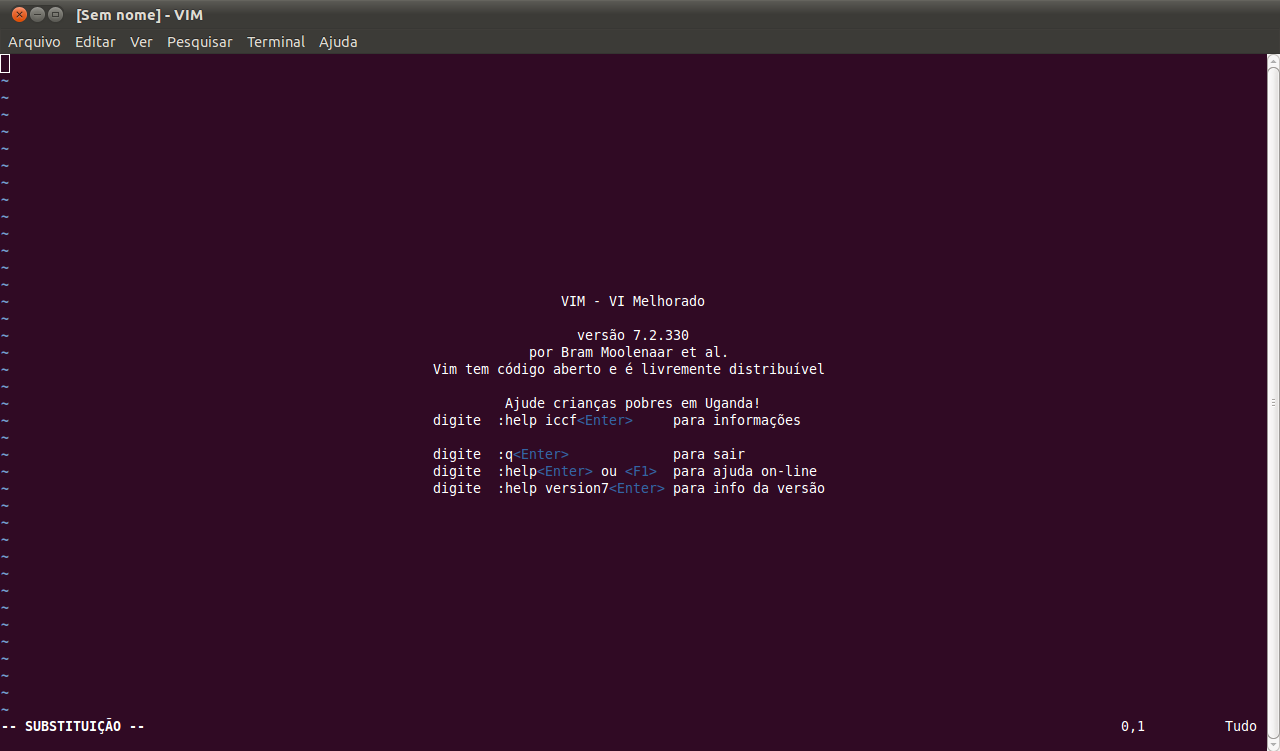
\includegraphics[height=6cm]{figures/vim_replace_screen}
    \caption{Tela após o comando \lcode{R}.}
    \label{fig:vim_replace_screen}
\end{figure}

\subsection{Trocando palavras}
Para trocar a primeira ocorrência de uma palavra por outra pode-se utilizar a sintaxe
\begin{code}
    :s/antiga/nova
\end{code}
onde \lcode{antiga} corresponde a palavra a ser substituida e \lcode{nova} a palavra que será utilizada para fazer a troca.

Para substituir todas as ocorrências de uma palavra em uma linha pode-se utilizar
\begin{code}
    :s/antiga/nova/g
\end{code}
e para todo o documento
\begin{code}
    :%s/antiga/nova/g
\end{code}

\subsection{Copiar, colar}
O comando \lcode{yy} ou \lcode{Y} copia a linha atual.

O comando \lcode{p} cola após o cursor e \lcode{P} antes a última informação copiada ou deletada.

\subsection{Inserindo arquivos}
Para inserir o conteudo de um arquivo no atual deve-se utilizar o comando
\begin{code}
    :r file
\end{code}
onde \lcode{file} é o nome do arquivo a ser inserido.

\section{Desfazer}
O comando \lcode{u} ou \lcode{:undo} desfaz a última alteração no texto. É permitido utilizar a tecla \lcode{u} mais de uma vez e com isso as alterações mais antigas são desfeitas. 

Ao errar em desfazer uma alteração pode-se utilizar as teclas \lcode{Ctrl}+\lcode{r} ou o comando \lcode{:redo}.


% Comandos avançados
% Filename: p2_advanced_vim@latex_with_vim.tex
% This code is part of LaTeX with Vim.
% 
% Description: LaTeX with Vim is free book about Vim, LaTeX and Git.
% 
% Created: 29.03.12 11:27:09 PM
% Last Change: 29.03.12 11:28:14 PM
% 
% Author: Raniere Gaia Costa da Silva, r.gaia.cs@gmail.com
% Organization:  
% 
% Copyright (c) 2010, 2011, 2012, Raniere Gaia Costa da Silva. All rights 
% reserved.
% 
% This file is license under the terms of a Creative Commons Attribution 
% 3.0 Unported License, or (at your option) any later version. More details
% at <http://creativecommons.org/licenses/by/3.0/>.
\chapter{Comandos avançados} \label{sch:vim:advance}
\section{Usando a \textit{shell}}

Para acessar a \textit{shell} sem fechar o Vim pode-se utilizar o comando \lcode{:sh}. Para retornar ao Vim deve-se utilizar os comandos \lcode{Ctrl}+\lcode{d} ou \lcode{exit}.

Para executar um comando da \textit{shell} diretamente do Vim deve-se utilizar o comando \lcode{:!} seguido pelo comando da \textit{shell}.

\section{Trabalhando com vários arquivos}
O Vim permite trabalhar com vários arquivos. Para abrir vários arquivos apresentando um em cima do outro, como apresentado na Figura \ref{fig:vim_vsplit_screen},
\begin{figure}[h!]
    \centering
    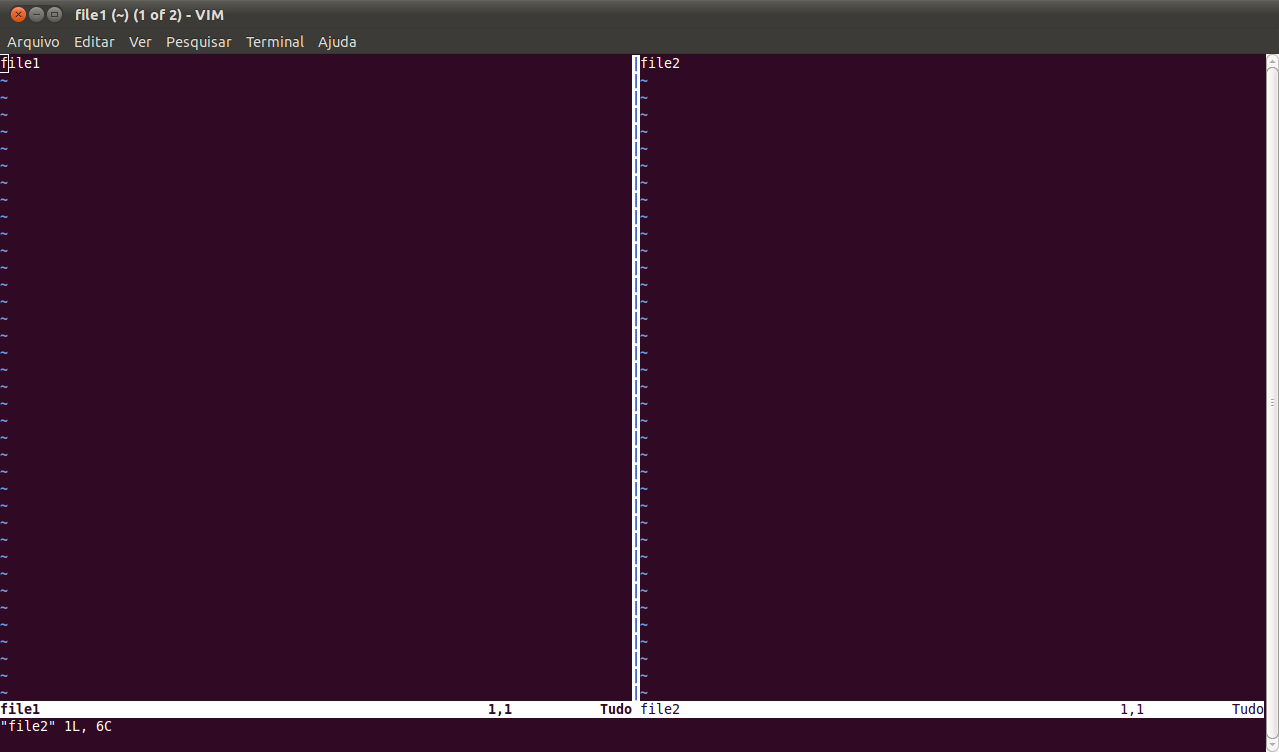
\includegraphics[height=6cm]{figures/vim_vsplit_screen}
    \caption{Dois arquivos separados verticalmente.}
    \label{fig:vim_vsplit_screen}
\end{figure}
pode-se utilizar, na \textit{shell}, o comando
\begin{code}
    vim -o file1 file2
\end{code}
e no caso do Vim já estar aberto utilizar o comando \lcode{:vsplit} .
Já para abrir vários arquivos apresentando um ao lado do outro, como apresentado na Figura \ref{fig:vim_split_screen},
\begin{figure}[h!]
    \centering
    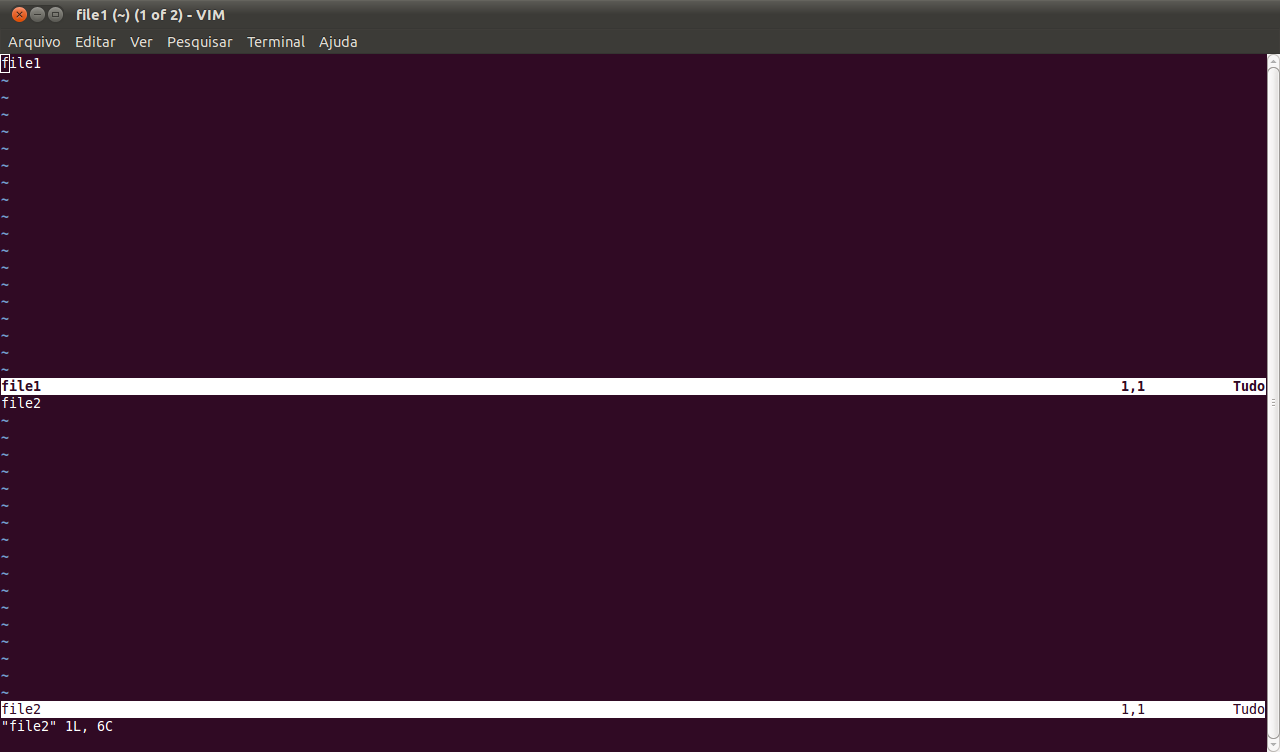
\includegraphics[height=6cm]{figures/vim_split_screen}
    \caption{Dois arquivos separados horizontalmente.}
    \label{fig:vim_split_screen}
\end{figure}
pode-se utilizar, na \textit{shell}, o comando
\begin{code}
    vim -O file1 file2
\end{code}
e no caso do Vim já estar aberto utilizar o comando \lcode{:split} .
E para apresentá-los sobrepostos pode-se utilizar, na \textit{shell}, o comando
\begin{code}
    vim file1 file2
\end{code}
e no caso do Vim já estar aberto utilizar o comando \lcode{:open} .

A movimentação entre as subjanelas ocorre pelos comandos \lcode{Ctrl}+\lcode{w} seguido da direção da ``nova'' subjanela em relação a ``antiga''. Já a movimentação os arquivos ocorre pelos comandos \lcode{:bn}, para o próximo arquivo, \lcode{:bp}, para o arquivo anterior, e \lcode{:b} seguido do número respectivo arquivo que deseja-se acessar.

Para listar os arquivos deve-se utilizar o comando \lcode{:ls}.

\section{Comparando arquivos}
Para comparar dois arquivos pode-se utilizar, na \textit{shell}, o comando
\begin{code}
    vim -d file1 file2
\end{code}
onde \lcode{file1} e \lcode{file2} são os nomes dos arquivos a serem comparados.
\begin{figure}[h!]
    \centering
    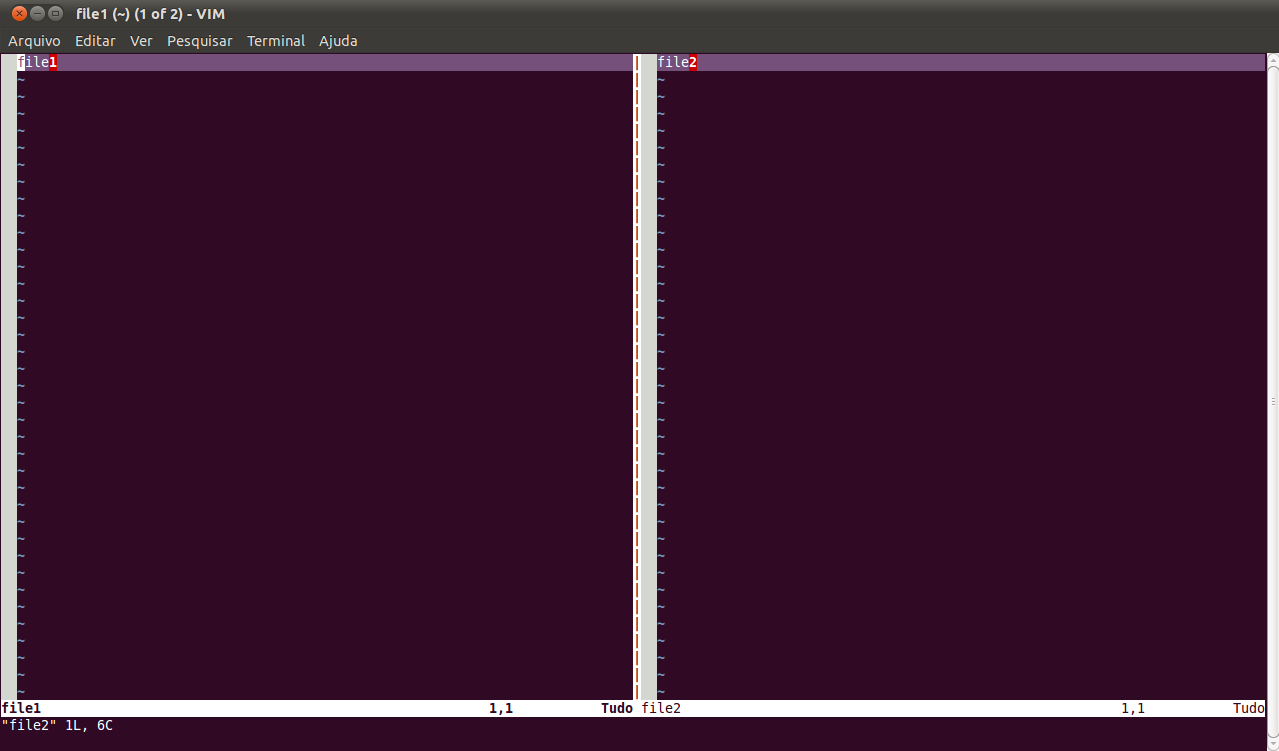
\includegraphics[height=6cm]{figures/vim_diff_screen}
    \caption{Tela de comparação de dois arquivos.}
    \label{fig:vim_diff_screen}
\end{figure}


\part{\LaTeX}
% Instalação
% Filename: p3_install@latex_with_vim.tex
% This code is part of LaTeX with Vim.
% 
% Description: LaTeX with Vim is free book about Vim, LaTeX and Git.
% 
% Created: 29.03.12 11:40:07 PM
% Last Change: 29.03.12 11:40:22 PM
% 
% Author: Raniere Gaia Costa da Silva, r.gaia.cs@gmail.com
% Organization:  
% 
% Copyright (c) 2010, 2011, 2012, Raniere Gaia Costa da Silva. All rights 
% reserved.
% 
% This file is license under the terms of a Creative Commons Attribution 
% 3.0 Unported License, or (at your option) any later version. More details
% at <http://creativecommons.org/licenses/by/3.0/>.
\chapter{Instalação} \label{sch:latex:install}
O LaTeX está disponível tanto no Windows, como nas distribuições Linux. A seguir, apresentaremos como proceder para instalar em ambos os sistemas operacionais.

\section{Windows}

A instalação no Windows ocorre em duas partes. Primeiramente deve-se instalar uma distribuição que possui as macros próprias do LaTex e, posteriormente, um editor ou IDE\footnote{Do inglês Integrated Development Environment ou Ambiente Integrado de Desenvolvimento, é um programa de computador que reúne características e ferramentas de apoio ao desenvolvimento de software, no nosso caso o texto, com o objetivo de agilizar este processo.} para LaTeX.

Uma das distribuições mais comuns para o Windows é o MikTeX, que pode ser baixado gratuitamente no site do projeto: \url{http://miktex.org/}. Outra distribuição, muito utilizada nas distribuições Linux, mas também disponível para Windows, é a TeX Live, que também pode ser baixada gratuitamente no site: \url{http://www.tug.org/texlive/}.

Quanto as IDE's para LaTeX, as opções são numerosas. Vamos apenas citar algumas e informar onde pode ser obtidas.
\begin{enumerate}
    \item Texmaker: \url{http://www.xm1math.net/texmaker/}
    \item WinEdt: \url{http://www.winedt.com/}
    \item TeXnicCenter: \url{http://www.texniccenter.org/}
    \item LED: \url{http://www.latexeditor.org/}\footnote{Alguns colegas relataram problemas ao utilizar o LED. Infelizmente ainda não verifiquei.}
    \item Winefish LaTeX Editor: \url{http://winefish.berlios.de/}
\end{enumerate}
Pessoalmente, gosto muito do Texmaker e alguns colegas gostam do WinEdt. De qualquer forma, a escolha da IDE é bastante pessoal e sugiro testar algumas antes de escolher uma.

\section{Linux}

A instalação em todas as distribuições Linux também passam pelas mesmas duas fases: instalação da distribuição e do editor/IDE. Felizmente, algumas distribuições já apresentam tanto uma distribuição instalada como um editor, caso contrário basta proceder com a instalação.

A instalação da distribuição no Ubuntu pode ser feita via terminal com o seguinte comando:
\begin{code}
    sudo apt-get install texlive texlive-latex-extra texlive-lang-portuguese texlive-math-extra
\end{code}
e, quanto a IDE, algumas das citadas anteriormente possuem versão para Linux.

Aos usuários que possuirem familiaridade com o Vim, sugiro darem uma olhada no VimLaTeX (\url{http://vim-latex.sourceforge.net/}), um conjunto de macros para o Vim voltadas para o LaTeX.


% Arquivo \textsf{.tex}
% Filename: p3_tex_file@latex_with_vim.tex
% This code is part of LaTeX with Vim.
% 
% Description: LaTeX with Vim is free book about Vim, LaTeX and Git.
% 
% Created: 29.03.12 11:46:11 PM
% Last Change: 29.03.12 11:46:27 PM
% 
% Author: Raniere Gaia Costa da Silva, r.gaia.cs@gmail.com
% Organization:  
% 
% Copyright (c) 2010, 2011, 2012, Raniere Gaia Costa da Silva. All rights 
% reserved.
% 
% This file is license under the terms of a Creative Commons Attribution 
% 3.0 Unported License, or (at your option) any later version. More details
% at <http://creativecommons.org/licenses/by/3.0/>.
\chapter{Arquivo \lcode{.tex}} \label{sch:latex:tex}
O LaTeX utiliza \lcode{.tex} como extensão padrão. O arquivo \lcode{MAIN.tex}, onde \lcode{MAIN} representa o nome do arquivo \lcode{.tex}, é um arquivo de texto, estruturado em duas partes:
\begin{enumerate}
    \item \textit{preâmbulo}
    \item \textit{informação}
\end{enumerate}
sendo que a segunda parte deve-se encontrar disposta no lugar de \lcode{XXX} do código abaixo:
\begin{latexcode}
    \begin{document}
    XXX
    \end{document}
\end{latexcode}

LaTeX permite incluir um arquivo dentro do \lcode{MAIN.tex}, isto é, trabalhar com múltiplos arquivos. Os arquivos a serem incluídos também possuem a extensão \lcode{.tex} mas devem conter apenas a \textit{informação}.\footnote{Ao trabalhar com múltiplos arquivos apenas precisa-se compilar o arquivo \lcode{MAIN.tex}.}

Nos próximos capítulos trataremos detalhadamente do \textit{preâmbulo} e da \textit{informação}. No momento, vamos tratar de como trabalhar com múltiplos arquivos.

\section{\textbackslash\lcode{input}}

A primeira forma de incluir um arquivo é com o comando \textbackslash\lcode{input}, como ilustrado a seguir:
\begin{latexcode}
    \input{aux}
\end{latexcode}
onde \lcode{aux} é o nome do arquivo a ser incluído.

Quando o arquivo principal for compilado o arquivo \lcode{aux.tex} será lido e processado exatamente como se tive-se sido inserido na posição que o comando \textbackslash\lcode{input} ocupa.

\section{\textbackslash\lcode{include}}

A segunda forma de incluir um arquivo é com o comando \textbackslash\lcode{include}, como ilustrado a seguir:
\begin{latexcode}
    \include{aux}
\end{latexcode}
onde \lcode{aux} é o nome do arquivo a ser incluído. Pode-se utilizar o comando \textbackslash\lcode{include} em conjunto com o comando \textbackslash\lcode{includeonly} para uma inclusão seletiva de arquivos.

Se o arquivo estiver listado no comando \textbackslash\lcode{includeonly} ou não existir tal comando, o comando \textbackslash\lcode{include} é equivalente a
\begin{latexcode}
    \clearpage \input{aux} \clearpage
\end{latexcode}
se o arquivo não estiver listado o comando \textbackslash\lcode{include} é equivalente a
\begin{latexcode}
    \clearpage
\end{latexcode}

Destaca-se que o comando \textbackslash\lcode{include} só pode ser utilizado no arquivo principal e nunca no \textit{preâmbulo}.


% Preâmbulo
% Filename: p3_preamble@latex_with_vim.tex
% This code is part of LaTeX with Vim.
% 
% Description: LaTeX with Vim is free book about Vim, LaTeX and Git.
% 
% Created: 29.03.12 11:44:40 PM
% Last Change: 30.03.12 12:03:46 AM
% 
% Author: Raniere Gaia Costa da Silva, r.gaia.cs@gmail.com
% Organization:  
% 
% Copyright (c) 2010, 2011, 2012, Raniere Gaia Costa da Silva. All rights 
% reserved.
% 
% This file is license under the terms of a Creative Commons Attribution 
% 3.0 Unported License, or (at your option) any later version. More details
% at <http://creativecommons.org/licenses/by/3.0/>.
\chapter{Preâmbulo} \label{sch:latex:preamble}
Neste capítulo abordaremos o \textit{preâmbulo} do arquivo \lcode{.tex} e a formatação da folha do documento a ser gerado.

\section{\textbackslash\lcode{documentclass} e \textbackslash\lcode{usepackage}}

O \textit{preâmbulo} deve ser iniciado por
\begin{latexcode}
    \documentclass[options]{class}
\end{latexcode}
onde \lcode{class} indica o tipo de documento a ser criado e \lcode{options} personaliza o compartamento de \lcode{class}. Os parâmetros para \lcode{options} devem ser separados por vírgula.

O parâmetro para \lcode{class} corresponde ao nome de um arquivo \lcode{.cls}, os principais são apresentados na Tabela \ref{tab:documentclass} e outros são indicados em \url{http://aprendolatex.wordpress.com/2007/07/15/mais-classes-de-documentos/}. Existe ainda alguns arquivos \lcode{.cls} personalizados disponíveis na internet, destacando-se o \lcode{abnt.cls}, disponível em \url{http://abntex.codigolivre.org.br/}, indicado para documentos que devem seguir as normas da ABNT.
\begin{table}[h!tb]
    \centering
    \caption{Parâmetros disponíveis para \lcode{class}.} \label{tab:documentclass}
    % Filename: documentclass@latex_with_vim.tex
% This code is part of LaTeX with Vim.
% 
% Description: LaTeX with Vim is free book about Vim, LaTeX and Git.
% 
% Created: 30.03.12 12:12:55 AM
% Last Change: 30.03.12 12:13:08 AM
% 
% Author: Raniere Gaia Costa da Silva, r.gaia.cs@gmail.com
% Organization:  
% 
% Copyright (c) 2010, 2011, 2012, Raniere Gaia Costa da Silva. All rights 
% reserved.
% 
% This file is license under the terms of a Creative Commons Attribution 
% 3.0 Unported License, or (at your option) any later version. More details
% at <http://creativecommons.org/licenses/by/3.0/>.
\begin{tabular}{lp{0.8\textwidth}}
    \hline
    Código & Descrição \\ \hline
    \lcode{article} & Para artigos em revistas especializadas, palestras, trabalhos de disciplinas \dots \\
    \lcode{report} & Para informes maiores que constam de mais de um capítulo, projetos de fim de curso, dissertações, teses e similares. \\
    \lcode{book} & Para livros. \\
    \lcode{slide} & Para transparências. \\
    \lcode{beamer} & Para apresenta\c{c}\~{o}es. \\
    \lcode{exam} & Para lista de exerc\'{i}cios. \\
    \hline
\end{tabular}

\end{table}

Na Tabela \ref{tab:par_options} encontramos alguns dos parâmetros disponíveis para \lcode{options}.
\begin{table}[h!tb]
    \centering
    \caption{Parâmetros disponíveis para \lcode{options}.}
    \label{tab:par_options}
    \begin{tabular}{llp{0.6\textwidth}}
        \hline
        Função & Código & Descrição \\ \hline
        \multirow{4}{*}{Tamanho} &  & Utiliza, por padrão, o tamanho 10. \\
        & \lcode{10pt} & Tamanho 10. \\
        & \lcode{11pt} & Tamanho 11. \\
        & \lcode{12pt} & Tamanho 12. \\ \hline
        \multirow{7}{*}{Papel} & & Utiliza, por padrão, o tamanho da folha correspondente carta. \\
        & \lcode{letterpaper} & Tamanho da folha correspondente carta. \\
        & \lcode{a4paper} & Tamanho da folha correspondente a A4. \\
        & \lcode{a5paper} & Tamanho da folha correspondente a A5. \\
        & \lcode{b5paper} & Tamanho da folha correspondente a B5. \\
        & \lcode{executivepaper} & Tamanho da folha correspondente a folha executiva. \\
        & \lcode{legalpaper} & Tamanho da folha correspondente a folha legal. \\ \hline
        \multirow{2}{*}{Al. equação} & & Por padrão centra as equações. \\
        & \lcode{fleqn} & Alinha as equações à esquerda. \\ \hline
        \multirow{2}{*}{Nº equação} & & Por padrão enumera as equações à direita. \\
        & \lcode{leqno} & Enumera as equações à esquerda. \\ \hline
        \multirow{4}{*}{Título} & & Por padrão a classe \lcode{article} não começa uma nova página após o título, enquanto que \lcode{report} e \lcode{book} o fazem. \\
        & \lcode{titlepage} & Começa uma nova página após o título. \\
        & \lcode{leqno} & Não começa uma nova página após o título. \\ \hline
        \multirow{4}{*}{Faces} & & Por padrão a classe \lcode{article} e \lcode{report} são a uma face e a classe \lcode{book} é a duas. \\
        & \lcode{oneside} & Gera o documento a uma face. \\
        & \lcode{twoside} & Gera o documento a duas fazes. \\ \hline
        \multirow{5}{*}{Começo} & & Não funciona com a classe \lcode{article} por nesta não existirem capítulos e por padrão a classe \lcode{report} começa os capítulos na próxima página disponível e a classe \lcode{book} sempre nas páginas à direita. \\
        & \lcode{openright} & Começa os capítulos sempre nas páginas à direita. \\
        & \lcode{openany} & Começa os capítulos na próxima página disponível. \\ \hline
        Colunas & \lcode{twocolumn} & Gera o arquivo utilizando-se de duas colunas. \\
        \hline
    \end{tabular}
\end{table}

O \textit{preâmbulo} do arquivo \lcode{.tex} é completado com os comandos para ativação dos pacotes que adicionam melhorias ao LaTeX que serão utilizados na \textit{informação}. O comando para ativação dos pacotes segue a seguinte sintaxes:
\begin{latexcode}
    \usepackage[options]{package}
\end{latexcode}
onde \lcode{package} é o nome do pacote a ser ativado e \lcode{options} é uma lista de palavras chaves que ativam funções especiais do pacote.

Neste ponto, vale destacar que as distribuições MikTeX e TeX Live possuem os pacotes de uso mais frequentes, mas algumas vezes pode ser necessário baixar o pacote requisitado. No CTAN (The Comprehensive TeX Archive Network: \url{http://www.ctan.org/}) é possível encontrar vários pacotes e a documentação dos mesmos.\footnote{Ao longo do livro, quando for necessário o uso de algum pacote faremos a indicação do mesmo.}

\section{Margens e estilo}

Para cada opção de papel definido em \textbackslash\lcode{documentclass} existe valores padrões para as margens. A seguir, mostraremos algumas maneiras de modificar tais valores e em seguida abordaremos os estilos das páginas.

\subsection{\textbackslash\lcode{setlength} e \textbackslash\lcode{addtolength}}

O comando
\begin{latexcode}
    \setlength{parameter}{length}
\end{latexcode}
atribui o valor \lcode{length} a \lcode{parameter} enquanto que o comando
\begin{latexcode}
    \addtolength{parameter}{length}
\end{latexcode}
adiciona o valor \lcode{length} ao valor padrão correspondente ao \lcode{parameter}.

Para \lcode{length} pode-se utilizar qualquer unidade suportada pelo LaTeX e os \lcode{parameter} disponíveis são apresentados na Tabela \ref{tab:par_margem} e ilustrados na Figura \ref{fig:par_margem}.
\begin{table}[h!tb]
    \centering
    \caption{Opções disponíveis para \lcode{parameter}.}
    \label{tab:par_margem}
    \begin{tabular}{lp{0.8\textwidth}}
        \hline
        Código & Descrição \\ \hline
        \textbackslash\lcode{hotset} & Valor a ser adicionado a margem lateral padrão de uma polegada. \\
        \textbackslash\lcode{votset} & Valor a ser adicionado a margem superior padrão de uma polegada. \\
        \textbackslash\lcode{evensidemargin} & Distância entre a margem lateral e a caixa de texto. \\
        \textbackslash\lcode{topsidemargin} & Distância entre a margem superior e o cabeçalho. \\
        \textbackslash\lcode{headheight} & Altura do cabeçalho. \\
        \textbackslash\lcode{headsep} & Distância entre o cabeçalho e a caixa de texto. \\
        \textbackslash\lcode{textheight} & Altura da caixa de texto. \\
        \textbackslash\lcode{textwidth} & Largura da caixa de texto. \\
        \textbackslash\lcode{marginparsep} & Distância entre a caixa de texto e as notas laterais \\
        \textbackslash\lcode{marginparwidth} & Largura das notas laterais \\
        \textbackslash\lcode{footskip} & Limite inferior para notas de rodapé. \\ \hline
    \end{tabular}
\end{table}
\begin{figure}[h!]
    \centering
    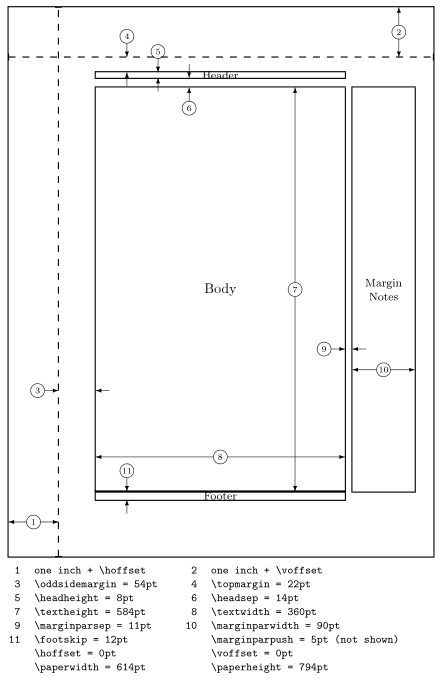
\includegraphics[height=15cm]{figures/margin.png}
    \flushright Fonte: \cite{Graetzer:2007:MoreMath}
    \caption{Ilustração da opções disponíveis para \lcode{parameter} apresentadas na Tabela \ref{tab:par_margem}.} \label{fig:par_margem}
\end{figure}

\subsection{\lcode{geometry}}

Outra maneira de configurar as margens é utilizando o pacote \lcode{geometry}. O uso deste pacote é bastante simples, precisa-se apenas fazer a chamada do pacote e atribuir valores para os parâmetros disponíveis. A seguir apresentamos um exemplo:
\begin{latexcode}
    \usepackage{geometry}
    \geometry{parameter = length, ...}
\end{latexcode}

Assim como para \textbackslash\lcode{setlength} e \textbackslash\lcode{addtolength} podemos utilizar \lcode{length} em qualquer unidade disponível no LaTeX. Já as opções para \lcode{parameter} mais utilizadas são apresentadas na Tabela \ref{tab:par_geometry} e ilustradas na Figura \ref{fig:par_geometry}.
\begin{table}[h!tb]
    \centering
    \caption{Opções disponíveis para \lcode{parameter}, referente ao pacote \lcode{geometry}.}
    \label{tab:par_geometry}
    \begin{tabular}{lp{0.8\textwidth}}
        \hline
        Código & Descrição \\ \hline
        \lcode{paperwidth} & Largura do papel. \\
        \lcode{paperheight} & Altura do papel. \\
        \lcode{textwidth} & Largura da caixa de texto. \\
        \lcode{textheigth} & Altura da caixa de texto. \\
        \lcode{top} & Margem superior. \\
        \lcode{bottom} & Margem inferior. \\
        \lcode{lefth} & Margem esquerda. \\
        \lcode{right} & Margem direita. \\ \hline
    \end{tabular}
\end{table}
\begin{figure}[h!]
    \centering
    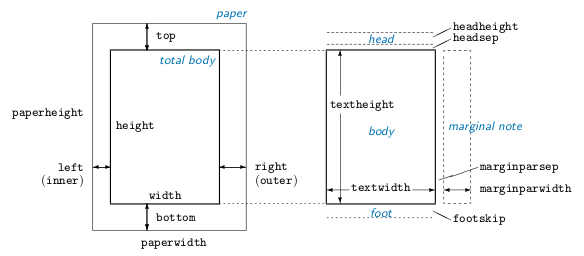
\includegraphics[width=0.8\textwidth]{figures/geometry_margin.png}
    \flushright Fonte: \cite{Moses:2007:Listings}
    \caption{Ilustração da opções disponíveis para \lcode{parameter} apresentadas na Tabela \ref{tab:par_geometry}.} \label{fig:par_geometry}
\end{figure}

\subsection{\textbackslash\lcode{pagestyle}}

Existe um estilo de página definido como padrão\footnote{Corresponde ao estilo \lcode{plain} apresentado na Tabela \ref{tab:par_style}.}, quando deseja-se mudar o estilo em todo o documento pode-se utilizar o comando
\begin{latexcode}
    \pagestyle{style}
\end{latexcode}
e quando for necessário mudá-lo apenas na página atual utiliza-se o comando
\begin{latexcode}
    \thispagestyle{style}
\end{latexcode}

As opções para \lcode{style} são apresentadas na Tabela \ref{tab:par_style}.
\begin{table}[!htb]
    \centering
    \caption{Opções disponíveis para \lcode{style}.}
    \label{tab:par_style}
    \begin{tabular}{lp{0.8\textwidth}}
        \hline
        Código & Descrição \\ \hline
        \lcode{plain} & Imprime os números de página no centro do pé da página. \\
        \lcode{headings} & No cabeçalho de cada página imprime o capítulo que está sendo processado e o número da página. O pé da página fica vazio. \\
        \lcode{empty} & Coloca tanto o cabeçalho como o pé da página vazios.
    \end{tabular}
\end{table}

Aos interessados em criar um estilo próprio, sugere-se utilizar o pacote \lcode{fancyhdr}.


% Hello world
% Filename: p3_hello_world@latex_with_vim.tex
% This code is part of LaTeX with Vim.
% 
% Description: LaTeX with Vim is free book about Vim, LaTeX and Git.
% 
% Created: 29.03.12 11:37:53 PM
% Last Change: 29.03.12 11:39:37 PM
% 
% Author: Raniere Gaia Costa da Silva, r.gaia.cs@gmail.com
% Organization:  
% 
% Copyright (c) 2010, 2011, 2012, Raniere Gaia Costa da Silva. All rights 
% reserved.
% 
% This file is license under the terms of a Creative Commons Attribution 
% 3.0 Unported License, or (at your option) any later version. More details
% at <http://creativecommons.org/licenses/by/3.0/>.
\chapter{Hello world} \label{sch:latex:hello_world}
Nos capítulos anteriores foi apresentado quais os aplicativos necessários para trabalhar com LaTeX e como instalá-los, as duas partes principais do arquivo \lcode{.tex} e descrevemos o \textit{preâmbulo}. Apartir deste capítulo abordaremos a segunda parte do arquivo \lcode{.tex} denominada de \textit{informação} que corresponde ao texto a ser gerado e neste primeiro momento apresentaremos os mais básicos conhecimentos necessários.

\section{O teclado}

Em todos os teclados encontramos as 52 letras (26 letras minúsculas + 26 letras maiúsculas) do alfabeto americano, os dez dígitos indo-arábicos, seis sinais de pontuação (\verb+ , ; . ? ! : +) e quatro parenteses (\verb+ ( ) [ ] +). Todos estas teclas são interpretadas como elas mesmas pelo LaTeX.

Na seção \ref{sss:latex:babel} abordaremos como o LaTeX interpreta o espaço e enter (mudança de linha).

As teclas correspondentes a \verb+ ` +, acento grave, \verb+ ' +, apóstrofe, e \verb+ - +, hífen, são interpretadas pelo LaTeX de acordo com os caracteres adjacentes.

Os seis símbolos matemáticos (\verb: * + = < > / :) são interpretados de maneira diferentes quando no modo texto e no modo matemático\footnote{O modo matemático é apresentado nos capítulos \ref{sch:latex:math1}, \ref{sch:latex:math2}, \ref{sch:latex:math3} e \ref{sch:latex:math4}}.

Existem, também, 13 símbolos especiais (\verb+ # $ % & ~ _ ^ \ { } @ " |+) que são interpretados pelo LaTeX de acordo com os caractéres adjacentes.

Os demais caracteres disponíveis no teclado, quando utilizados, costumam produzir erro.

\section{Idioma} \label{sss:latex:babel}
O LaTeX foi desenvolvido inicialmente para o idioma inglês e, por isso, sua utilização em outros idiomas, pode ser um pouco complicada. Para facilitar o uso do LaTeX em outros idiomas pode-se utilizar o pacote \lcode{babel} de Johannes L. Braams.

Para que o pacote \lcode{babel} funcione adequadamente, deve-se configurar o LaTeX de uma forma especial de acordo com codificação utilizada pelo arquivo \lcode{.tex}. As codificações mais comuns são Latin1 e UFT-8\footnote{O pacote \lcode{listings} não funciona adequadamente com esta codificação e por isso é fortemente aconcelhável utilizar a codificação Latin1.} sendo que para arquivos codificados com Latin1 deve-se adicionar a seguinte linha no preâmbulo
\begin{latexcode}
    \usepackage[latin1]{inputenc}
\end{latexcode}
enquanto que para arquivos codificados com UFT-8
\begin{latexcode}
    \usepackage[utf8]{inputenc}
\end{latexcode}

É importante que o editor que esteja sendo usado também esteja configurado para trabalhar com a codificação especificada. Quando uma codificação errada estiver sendo usada, o editor pode trocar ou omitir alguns caracteres.

Está disponível no pacote \lcode{babel} as seguintes opções para o idioma português: \lcode{portuges}, \lcode{portuguese}, \lcode{brazil}, \lcode{brazilian}. As opções definem alguns ajustes referentes a traduções de alguns termos e uso de caixa alta e maiores detalhes podem ser encontrados em \cite{Braams:2008:Babel}.

Em resumo, para os usuários que trabalham no Windows as seguintes linhas de código devem ser adicionas ao preâmbulo
\begin{latexcode}
    \usepackage[latin1]{inputenc}
    \usepackage[brazil]{babel}
\end{latexcode}
enquanto que os usuários do Linux
\begin{latexcode}
    \usepackage[utf8]{inputenc}
    \usepackage[brazil]{babel}
\end{latexcode}

\section{Primeiro documento}

Com o que foi apresentado agora é possível gerar a saída para um arquivo \lcode{.tex} bem simples. \\ 
\begin{minipage}[t]{0.47\linewidth}
    \vspace{-8pt}
    \begin{latexcode}
        \documentclass[10pt,a4paper]{article}
        \begin{document}
        Hello world.
        \end{document}
    \end{latexcode}
\end{minipage} \hfill
\begin{minipage}[t]{0.47\linewidth} \vspace{0pt}
    Hello world.
\end{minipage}

Os exemplos que serão apresentados aparecerão seguindo o modelo acima, isto é, em duas colunas sendo a coluna da esquerda contendo o código LaTeX e a coluna da direita contendo a saída obtida. Por simplicidade, nos demais exemplos iremos apresentar apenas a \textit{informação}.

\section{Espaços, linhas, parágrafos e páginas} \label{sss:lates:space}

No LaTeX o espaço entre palavras apresenta uma particularidade, ao compilar o \lcode{MAIN.tex}, ele ignora dois ou mais espaços seguidos, como podemos observar a seguir.. \\
\begin{minipage}[t]{0.47\linewidth} \vspace{-8pt}
    \begin{latexcode}
        Hello  world.(2 spaces)
        Hello   world.(3 spaces)
    \end{latexcode}
\end{minipage} \hfill
\begin{minipage}[t]{0.47\linewidth} \vspace{0pt}
    Hello  world.(2 spaces)
    Hello   world.(3 spaces)
\end{minipage}

Quando for necessário gerar dois ou mais espaços seguidos deve-se utilizar a barra invertida entre os espaços como ilustrado a seguir. \\
\begin{minipage}[t]{0.47\linewidth} \vspace{-8pt}
    \begin{latexcode}
        Hello \ world.(2 spaces)
        Hello \ \ world.(3 spaces)
    \end{latexcode}
\end{minipage} \hfill
\begin{minipage}[t]{0.47\linewidth} \vspace{0pt}
    Hello \ world.(2 spaces)
    Hello \ \ world.(3 spaces)
\end{minipage}

Nos dois exemplos anteriores é possível verificar que a mudança de linha no código não produz uma nova linha no documento gerado. A mudança de linha no LaTeX é representada pelos comandos \textbackslash\textbackslash \ ou \textbackslash\lcode{newline}, como ilustrada a seguir. \\
\begin{minipage}[t]{0.47\linewidth} \vspace{-8pt}
    \begin{latexcode}
        Hello world.[1] \\
        Hello world.[2] \newline
        Hello world.[3]
    \end{latexcode}
\end{minipage} \hfill
\begin{minipage}[t]{0.47\linewidth} \vspace{0pt}
    Hello world.[1] \\
    Hello world.[2] \newline
    Hello world.[3]
\end{minipage}

Já a mudança de parágrafo é indicada por uma linha em branco. 

Quando for necessário forçar uma mudança de página utiliza-se o comando \textbackslash\lcode{newpage}. Assim como o LaTeX ignora dois ou mais espaços seguidos a mudança de linha e de página também é ignorada.

Por último é importante avisar que, uma regra tipográfica padrão, o primeiro parágrafo de  capítulo, seções, \dots, não é identado. Quando desejar-se identar o primeiro parágrago uma solução é utilizar o pacote \lcode{indentfirst}.

\section{Hifenização}

O LaTeX tenta balancear o tamanho das linhas a serem geradas e para isso utiliza-se de um banco de dados para hifenizar, quando necessário, alguma palavra.

Algumas vezes a hifenização ocorre de maneira inadequada e para corrigir devemos utilizar o comando \textbackslash\lcode{hyphenation} cujo parâmetro é uma lista de palavras, separadas por espaço, onde o comando - é utilizado para indicar onde a palavra pode ser separada.

\section{Acentos}
Para a acentuação deve-se proceder como na Tabela \ref{tab:diacritic}. Quando utilizado o pacote \lcode{babel}, apresentado na seção \ref{sss:latex:babel}, pode-se também proceder normalmente.
\begin{table}[!htb]
    \centering
    \caption{Acentuação (utilizando a vogal ``o'' para exemplo).} \label{tab:diacritic}
    % Filename: diacrict@latex_with_vim.tex
% This code is part of LaTeX with Vim.
% 
% Description: LaTeX with Vim is free book about Vim, LaTeX and Git.
% 
% Created: 30.03.12 12:12:36 AM
% Last Change: 30.03.12 12:12:40 AM
% 
% Author: Raniere Gaia Costa da Silva, r.gaia.cs@gmail.com
% Organization:  
% 
% Copyright (c) 2010, 2011, 2012, Raniere Gaia Costa da Silva. All rights 
% reserved.
% 
% This file is license under the terms of a Creative Commons Attribution 
% 3.0 Unported License, or (at your option) any later version. More details
% at <http://creativecommons.org/licenses/by/3.0/>.
\begin{tabular}{cc|cc|cc|cc}
    \hline
    Comando & Resultado & Comando & Resultado & Comando & Resultado & Comando & Resultado \\ \hline
    \textbackslash '\{o\} & \'{o} & \textbackslash =\{o\} & \={o} & \textbackslash u\{o\} & \u{o} & \textbackslash .\{o\} & \.{o} \\
    \textbackslash v\{o\} & \v{o} & \textbackslash r\{o\} & \r{o} & \textbackslash c\{c\} & \c{c} & \textbackslash t\{oo\} & \t{oo} \\
    \textbackslash \textasciicircum \{o\} & \^{o} & \textbackslash \textasciitilde \{o\} & \~{o} & \textbackslash "\{o\} & \"{o} & \textbackslash d\{o\} & \d{o} \\
    \textbackslash H\{o\} & \H{o} & \textbackslash b\{o\} & \b{o} & \textbackslash `\{o\} & \`{o} & \textbackslash i & \i \\ \hline
\end{tabular}

\end{table}

\section{Caracteres especiais}
No LaTeX alguns caracteres apresentam forma própria de representação. A seguir enunciaremos alguns.

\subsection{Aspas}
Para as aspas não deve-se usar o caracter de aspas. Para abrir as aspas deve-se utilizar o acento simples e para fechar a aspa simples. \\
\begin{minipage}[t]{0.47\linewidth} \vspace{-8pt}
    \begin{latexcode}
        `Hello world.' (aspas simples) \\
        ``Hello world.'' (aspas dupla) \\
        "Hello world." (errado)
    \end{latexcode}
\end{minipage} \hfill
\begin{minipage}[t]{0.47\linewidth} \vspace{0pt}
    `Hello world.' (aspas simples) \\
    ``Hello world.'' (aspas dupla) \\
    "Hello world." (errado)
\end{minipage}

\subsection{Traço}
LaTeX admite três tipos de traço. \\
\begin{minipage}[t]{0.47\linewidth} \vspace{-8pt}
    \begin{latexcode}
        sem-terra \\
        08--10 hours \\
        Campinas --- SP
    \end{latexcode}
\end{minipage} \hfill
\begin{minipage}[t]{0.47\linewidth} \vspace{0pt}
    sem-terra \\
    08--10 hours \\
    Campinas --- SP
\end{minipage}

\subsection{Pontos sucessivos}
Utiliza-se o comando \textbackslash\lcode{dots} ou \textbackslash\lcode{ldots} para pontos sucessivos. \\
\begin{minipage}[t]{0.47\linewidth} \vspace{-8pt}
    \begin{latexcode}
        patatoes, carrots \ldots (correta) \\
        patatoes, carrots \dots (correta) \\
        patatoes, carrots ... (errada) \\
    \end{latexcode}
\end{minipage} \hfill
\begin{minipage}[t]{0.47\linewidth} \vspace{0pt}
    patatoes, carrots \ldots (correta) \\
    patatoes, carrots \dots (correta) \\
    patatoes, carrots ... (errada) \\
\end{minipage}

\subsection{Pontuação e demais símbolos}
Para pontuação e demais símbolos especias deve-se proceder como na Tabela \ref{tab:symbols}.
\begin{table}[h!tb]
    \centering
    \caption{Para pontuação e símbolos especias.}
    \label{tab:symbols}
    % File: symbols@latex-with-vim.tex
% This code is part of LaTeX with Vim.
% 
% Description: LaTeX with Vim is free book about Vim, LaTeX and Git.
% 
% Created: 30.03.12 12:19:38 AM
% Last Change: 30.03.12 12:19:44 AM
% 
% Author: Raniere Gaia Costa da Silva, r.gaia.cs@gmail.com
% Organization:  
% 
% Copyright (c) 2010, 2011, 2012, Raniere Gaia Costa da Silva. All rights 
% reserved.
% 
% This file is license under the terms of a Creative Commons Attribution 
% 3.0 Unported License, or (at your option) any later version. More details
% at <http://creativecommons.org/licenses/by/3.0/>.

\begin{tabular}{cc|cc|cc}
    \hline
    Comando & Resultado & Comando & Resultado & Comando & Resultado \\ \hline
    \textbackslash \& & \& & \textbackslash textasteriskcentered & \textasteriskcentered & \textbackslash textbackslash & \textbackslash \\
    \textbackslash textbar & \textbar & \textbackslash \{ & \{ & \textbackslash \} & \} \\
    \textbackslash texbullet & \textbullet & \textbackslash textasciitilde & \textasciitilde & \textbackslash textasciicircum & \textasciicircum \\
    \textbackslash copyright & \copyright & \textbackslash textregistered & \textregistered & \textbackslash texttrademark & \texttrademark \\
    \textbackslash textperiodcentered & \textperiodcentered & \textbackslash textexclamdown & \textexclamdown & \textbackslash textquestiondown & \textquestiondown \\
    \textbackslash \% & \% & \textbackslash textgreater & \textgreater & \textbackslash textless & \textless  \\
    \textbackslash \# & \# & \textbackslash S & \S & \textbackslash P & \P \\
    \textbackslash \_ & \_ & \textbackslash dag & \dag & \textbackslash ddag & \ddag \\
    \textbackslash pounds & \pounds & \textbackslash textsuperscript\{a\} & \textsuperscript{a} & \textbackslash textcircled\{a\} & \textcircled{a} \\
    \textbackslash textvisiblespace & \textvisiblespace & \textbackslash \$ & \$ & \textbackslash euro & \euro \\ \hline
\end{tabular}

\end{table}

Destaca-se que para que o símbolo \euro \ seja impresso é necessário que o \textit{preâmbulo} contenha a seguinte linha de código
\begin{latexcode}
    \usepackage[official]{eurosym}
\end{latexcode}

\section{Comentários}
Também é possível inserir comentários no arquivo \lcode{.tex}, utilizando-se para isso do caractere \% de forma que todo o texto posterior ao mesmo e na mesma linha é considerado comentário e não é processado. \\
\begin{minipage}[t]{0.47\linewidth} \vspace{-8pt}
    \begin{latexcode}
        Hello world.%comentario
    \end{latexcode}
\end{minipage} \hfill
\begin{minipage}[t]{0.47\linewidth} \vspace{0pt}
    Hello world.%comentario
\end{minipage}


% Trabalhando um texto: Parte 1
% Filename: p3_text_basic@latex_with_vim.tex
% This code is part of LaTeX with Vim.
% 
% Description: LaTeX with Vim is free book about Vim, LaTeX and Git.
% 
% Created: 29.03.12 11:47:22 PM
% Last Change: 30.03.12 12:07:34 AM
% 
% Author: Raniere Gaia Costa da Silva, r.gaia.cs@gmail.com
% Organization:  
% 
% Copyright (c) 2010, 2011, 2012, Raniere Gaia Costa da Silva. All rights 
% reserved.
% 
% This file is license under the terms of a Creative Commons Attribution 
% 3.0 Unported License, or (at your option) any later version. More details
% at <http://creativecommons.org/licenses/by/3.0/>.
\chapter{Trabalhando um texto: Parte 1} \label{css:latex:text-basic}
Neste capítulo apresentaremos as ferramentas do LaTeX disponíveis para organizar um texto. Começaremos pela modificação da fonte utilizada e como fazer citações.

Ao fim do capítulo abordaremos a escrita de versos.

\section{Fonte}
No LaTeX estão disponíveis algumas fontes opcionais. Comandos da forma \textbackslash\lcode{textXX} são responsáveis por alterar a fonte sendo que \lcode{XX} corresponde ao código da fonte a serem utilizados. A Tabela \ref{tab:text} apresenta alguns das opções disponíveis.
\begin{table}[!htb]
    \centering
    \caption{Opções disponíveis para \lcode{XX} da fonte.} \label{tab:text}
    % Filename: text@latex_with_vim.tex
% This code is part of LaTeX with Vim.
% 
% Description: LaTeX with Vim is free book about Vim, LaTeX and Git.
% 
% Created: 30.03.12 12:19:02 AM
% Last Change: 30.03.12 12:19:06 AM
% 
% Author: Raniere Gaia Costa da Silva, r.gaia.cs@gmail.com
% Organization:  
% 
% Copyright (c) 2010, 2011, 2012, Raniere Gaia Costa da Silva. All rights 
% reserved.
% 
% This file is license under the terms of a Creative Commons Attribution 
% 3.0 Unported License, or (at your option) any later version. More details
% at <http://creativecommons.org/licenses/by/3.0/>.
\begin{tabular}{lp{0.8\textwidth}}
    \hline
    Código & Descrição \\ \hline
    \lcode{it} & Texto em itálico. \\
    \lcode{bf} & Texto em negrito. \\
    \lcode{rm} & Texto em romano. \\
    \lcode{sf} & Texto em sans serif. \\
    \lcode{tt} & Texto na tipografia de uma máquina de escrever. \\
    \lcode{sc} & Texto em caixa alta. \\ \hline
\end{tabular}

\end{table}

A seguir é ilustrado as opções apresentadas na Tabela \ref{tab:text}. \\
\begin{minipage}[t]{0.47\linewidth} \vspace{-8pt}
    \begin{latexcode}
        Italico: \textit{novo texto}. \\
        Negrito: \textbf{novo texto}. \\
        Romano: \textrm{novo texto}. \\
        Sans serif: \textsf{novo texto}. \\
        Maquina de escrever: \texttt{novo texto}. \\
        Caixa alta: \textsc{novo texto}.
    \end{latexcode}
\end{minipage} \hfill
\begin{minipage}[t]{0.47\linewidth} \vspace{0pt}
    Italico: \textit{novo texto}. \\
    Negrito: \textbf{novo texto}. \\
    Romano: \textrm{novo texto}. \\
    Sans serif: \textsf{novo texto}. \\
    Maquina de escrever: \texttt{novo texto}. \\
    Caixa alta: \textsc{novo texto}.
\end{minipage}

\subsection{Edição direta}
Algumas vezes deseja-se inserir um texto que não deve ser interpretado. Isso é possível pelo ambiente \lcode{verbatim}, coloca o texto em uma nova linha, e pelo comando \textbackslash\lcode{verb}, coloca o texto no mesmo parágrafo.

Tanto o ambiente \lcode{verbatim} como o comando \textbackslash\lcode{verb} apresentam uma fonte própria. \\
\begin{minipage}[t]{0.47\linewidth} \vspace{-8pt}
    \begin{latexcode}
        \textsc{texto interpretado.} \\
        \verb+Texto nao interpretado.+
    \end{latexcode}
\end{minipage} \hfill
\begin{minipage}[t]{0.47\linewidth} \vspace{0pt}
    \textsc{texto interpretado.} \\
    \verb+Texto nao interpretado.+
\end{minipage}

Vale destacar que o comando \textbackslash\lcode{verb} é ``flexível'' quando ao delimitador, os caracteres \verb:+: e \verb+:+ normalmente exercem satisfatoriamente esta função.

\section{Tamanho}
Uma das maneiras de mudar o tamanho da fonte em uma parte do texto é utilizando um dos ambiente  ou comando de tamanho (a Tabela \ref{tab:op_tamanho_fonte} apresenta algumas opções disponíveis).
\begin{table}[h!tb]
    \centering
    \caption{Opções disponíveis para o tamanho da fonte, em ordem crescente.}
    \label{tab:op_tamanho_fonte}
    \begin{tabular}{lp{0.7\textwidth}}
        \hline
        Código & Descrição \\ \hline
        \lcode{tiny} & O menor tamanho possível. \\
        \lcode{SMALL} ou \lcode{scriptsize} &  \\
        \lcode{Small} ou \lcode{footnotesize} & Tamanho utilizado em notas de rodapé. \\
        \lcode{small} &  \\
        \lcode{normalsize} & Tamanho padrão. \\
        \lcode{large} & \\
        \lcode{Large} & \\
        \lcode{LARGE} & \\
        \lcode{huge} & \\
        \lcode{Huge} & O maior tamanho disponível. \\ \hline
    \end{tabular}
\end{table}

Destaca-se que os tamanhos são baseados no tamanho padrão. A seguir um exemplo. \\
\begin{minipage}[t]{0.47\linewidth} \vspace{-8pt}
    \begin{latexcode}
        {\tiny muito pequeno} \\
        {\small pequeno} \\
        fonte padrao \\
        {\Large grande} \\
        {\Huge enorme}
    \end{latexcode}
\end{minipage} \hfill
\begin{minipage}[t]{0.47\linewidth} \vspace{0pt}
    {\tiny muito pequeno} \\
    {\small pequeno} \\
    fonte padrao \\
    {\Large grande} \\
    {\Huge enorme}
\end{minipage}

\section{Cor}
Para alterar a cor do texto é necessário os pacotes \lcode{graphicx} e \lcode{color} e pode-se utilizar um dos comandos: \textbackslash\lcode{textcolor} ou \textbackslash\lcode{color}.

A seguir apresentamos um exemplo. \\
\begin{minipage}[t]{0.47\linewidth} \vspace{-8pt}
    \begin{latexcode}
        \textcolor{blue}{azul} \\
        {\color{blue}azul}
    \end{latexcode}
\end{minipage} \hfill
\begin{minipage}[t]{0.47\linewidth} \vspace{0pt}
    \textcolor{blue}{azul} \\
    {\color{blue}azul}
\end{minipage}

\section{Espaçamento}
Nesta seção abordaremos como inserir espaços ao longo do texto no LaTeX, mas antes é importante destacar que podemos suprimir espaços ao utilizar medidas negativas.

\subsection{Espaçamento horizontal}
Para produzir um espaço horizontal utiliza-se o comando \textbackslash\lcode{hspace} que tem como parâmetro o tamanho do espaço a ser inserido. Se o comando ocorrer entre duas linhas ou no início de uma linha o LaTeX não produz o espaço e para este caso devemos utilizar  \textbackslash\lcode{hspace}\textasteriskcentered.

Para modificar a identação característica de um novo parágrafo deve-se utilizar o comando
\begin{latexcode}
    \setlength{\parident}{tam}
\end{latexcode} 
onde \lcode{tam} é o novo tamanho para a identação dos parágrafos. No caso de desejar-se suprimir a identação deve-se utilizar o comando \textbackslash\lcode{noindent}.

O comando \textbackslash\lcode{hfill} cria um espaço suficiente para dividir o texto de modo que o que estiver antes do comando é alinhado a esquerda e o que estiver depois é alinhado a direita. É permitido utilizar o comando mais de uma vez em uma linha. O comando é ignorado quando ocorrer entre duas linhas ou no início de uma linha, neste caso devemos utilizar  \textbackslash\lcode{hfill}\textasteriskcentered.

\subsection{Linha horizontal}
Os comandos \textbackslash\lcode{dotfill} e \textbackslash\lcode{hrulefill} funcionam de maneira semelhante ao comando \textbackslash\lcode{hfill}, mas ao invés de inserir um espaço em branco é introduzido, respectivamente uma linha pontilhada e uma linha contínua.

\subsection{Espaçamento vertical}
No capítulo anterior informamos como mudar de linha, nesta seção vamos trabalhar com o espaço entre as linhas.

O comando \textbackslash\lcode{baselineskip[tam]} estabelece o tamanho do espaçamento entre linhas para o texto posterior ao comando. Para modificar o tamanho entre duas linhas específicas pode-se utilizar o comando \textbackslash\textbackslash\lcode{[tam]} inicia uma nova linha de maneira que \lcode{tam} é o espaçamento entre as linhas.

Para aumentar o espaço entre parágrafos pode-se utilizar os comandos \textbackslash\lcode{smallskip}, \textbackslash\lcode{medskip} ou \textbackslash\lcode{bigskip}, sendo que o tamanho do espaço está relacionado com o tamanho da fonte padrão do documento.

Os comandos \textbackslash\lcode{vspace} e \textbackslash\lcode{vfill} funcionam, respectivamente, de modo muito semelhante aos comandos \textbackslash\lcode{hspace} e \textbackslash\lcode{hfill} só que na vertical.

\section{Alinhamento}
Por padrão, o alinhamento ocorre com a margem esquerda e para alterá-lo pode-se utilizar um dos seguintes ambientes: \lcode{center} (para texto centralizado), \lcode{flushleft} (alinhamento a esquerda) e \lcode{flushright} (alinhamento a direita). \\
\begin{minipage}[t]{0.47\linewidth} \vspace{-8pt}
    \begin{latexcode}
        \begin{flushleft}esquerda
        \end{flushleft} \\
        \begin{center}centralizado
        \end{center} \\
        \begin{flushright}direita
        \end{flushright}
    \end{latexcode}
\end{minipage} \hfill
\begin{minipage}[t]{0.47\linewidth} \vspace{0pt}
    \begin{flushleft}esquerda
    \end{flushleft}
    \begin{center}centralizado
    \end{center}
    \begin{flushright}direita
    \end{flushright}
\end{minipage}

Também é permitido utilizar os comandos: \textbackslash\lcode{centering} (para texto centralizado), \textbackslash\lcode{raggedleft} (alinhamento a esquerda) e \textbackslash\lcode{raggedright} (alinhamento a direita).

\section{Texto em colunas}
Como vimos no Capítulo \ref{sch:latex:preamble}, podemos gerar um documento com duas colunas utilizando a opção \lcode{twocolumn} no comando \textbackslash\lcode{documentoclass}. Nesta seção abordaremos como introduzir duas ou mais colunas em um partes de um documento.

Antes de começar é importante informar que os ambientes a seguir informados para trabalhar com colunas não são $100$\% compatíveis com os comandos e ambientes do LaTeX e apenas o método de tentativa e erro para saber o que funciona.

\subsection{\textbackslash\lcode{twocolumn}}
O comando \textbackslash\lcode{twocolumn[nome]} termina a página atual e inicia uma nova página com duas colunas por página. O argumento opcional \lcode{nome} é escrito no início da página em uma coluna com a largura da página. O comando \textbackslash\lcode{onecolumn} termina o modo de duas colunas.

\subsection{\lcode{multicols}} \nocite{Mitttelbach:2009:Multicolumn}
O ambiente \lcode{multicols}, definido no pacote \lcode{multicols}, apresenta a seguinte sintaxe:
\begin{latexcode}
    \begin{multicols}{number}
        texto
    \end{multicols}
\end{latexcode}
onde \lcode{number} é o número de colunas a serem criadas.

\subsection{\lcode{parcolumns}} \nocite{Sauer:2004:Parcolumns}
O ambiente \lcode{parcolumns}, definido no pacote \lcode{parcolumns}, apresenta sintaxe muito semelhante ao ambiente \lcode{multicols}:
\begin{latexcode}
    \begin{parcolumns}[options]{number}
        texto
    \end{parcolumns}
\end{latexcode}
onde \lcode{number} é o número de colunas a serem criadas e \lcode{options} algumas configurações opcionais (para maiores informações procurar \cite{Sauer:2004:Parcolumns}).

\subsection{\lcode{parallel}}
Ao trabalhar, principalmente, com documentos bilingues é interessante utilizar cada coluna para um idioma e deixar parágrafos correspondentes alinhados. Para isso pode-se utilizar o ambiente \lcode{parallel}, definido no pacote \lcode{parallel}, que apresenta a seguinte sintaxe:
\begin{latexcode}
    \begin{Parallel}{col1}{col2}
        \ParallelLText{...}
        \ParallelRText{...}
        \ParallelPar
    \end{Parallel}
\end{latexcode}
onde \lcode{col1} e \lcode{col2} é a largura das colunas.

O comando \textbackslash\lcode{ParallelLText} tem como parâmetro o texto da coluna da esquerda enquanto que o comando \textbackslash\lcode{ParallelRText} o texto da coluna da direita e o comando \textbackslash\lcode{ParallelPar} indica o alinhamento dos parágrafos.

\subsection{\lcode{minipage}}
O ambiente \lcode{minipage} é responsável por criar pequenas páginas, caixas, ao longo do texto. A síntaxe do ambiente é
\begin{latexcode}
    \begin{minipage}[pos]{largura}
    \end{minipage}
\end{latexcode}
onde \lcode{pos} é a posição do texto que está na minipágina e \lcode{largura} é a largura da minipágina.

O ambiente \lcode{minipage} não apresenta borda, para incluí-la pode-se utilizar o ambiente \lcode{boxedminipage} definido no pacote \lcode{boxedminipage}.

Para simular colunas utilizando-se do ambiente \lcode{minipage} precisa-se apenas utilizar duas ou mais vezes o ambiente em sequência como indicadono código abaixo
\begin{latexcode}
    \begin{minipage}[pos1]{largura1}
        ...
    \end{minipage} espaco
    \begin{minipage}[pos1]{largura1}
        ...
    \end{minipage}
\end{latexcode}
onde \lcode{espaco} é um comando para distanciar uma coluna da outra.

Ao tentar simular colunas com o ambiente \lcode{minipage} pode ocorrer que o texto de uma coluna inicie apenas ao fim do texto da outra coluna. Para resolver este problema deve-se adicionar o comando \textbackslash\lcode{vspace\{0pt\}} no início de cada \lcode{minipage}.

O ambiente \lcode{minipage}, ao contrário dos apresentados anteriormente, é tratado como um objeto flutuante de modo que seu conteudo não pode ser dividido entre páginas requerendo um pouco mais de atenção.


% Trabalhando um texto: Parte 2
% Filename: p3_text_advanced@latex_with_vim.tex
% This code is part of LaTeX with Vim.
% 
% Description: LaTeX with Vim is free book about Vim, LaTeX and Git.
% 
% Created: 29.03.12 11:46:50 PM
% Last Change: 29.03.12 11:47:06 PM
% 
% Author: Raniere Gaia Costa da Silva, r.gaia.cs@gmail.com
% Organization:  
% 
% Copyright (c) 2010, 2011, 2012, Raniere Gaia Costa da Silva. All rights 
% reserved.
% 
% This file is license under the terms of a Creative Commons Attribution 
% 3.0 Unported License, or (at your option) any later version. More details
% at <http://creativecommons.org/licenses/by/3.0/>.
\chapter{Trabalhando um texto: Parte 2} \label{C:text2}
Neste capítulo continuaremos apresentado algumas ferramentas do LaTeX disponíveis para organizar um texto, agora voltadas para textos matemáticos, e apresentaremos o ambeinte \textsf{minipage}.

\section{Nota de rodapé}

Para produzir notas de rodapé deve-se utilizar o comando \textbackslash\textsf{footnote} que deve ocorrer imediatamente depois da palavra ou texto a que se refere a nota de rodapé e como parâmetro do comando o texto a ser inserido na nota de rodapé.

\section{Referência cruzada} \label{sse:cross_reference}

Existem dois tipos de referência cruzada, a primeira para alguma parte do documento e a segunda para um outro documento. Nesta seção abordaremos o primeiro tipo e o segundo será trabalhado no Capítulo~\ref{sch:latex::bibtex}.

Para alguns comandos e ambientes o LaTeX atribui um número que pode ser vinculado a um nome pelo comando \textbackslash\textsf{label} e referenciado pelo comando \textbackslash\textsf{ref} ou \textbackslash\textsf{pageref}, para a página onde encontra-se o item referenciado.

O argumento do comando \textbackslash\textsf{label} é uma sequencia de caracteres\footnote{Recomenda-se escolher uma sequencia ``amigável''}, case sensitive, que será utilizada como argumento do comando \textbackslash\textsf{ref} ao efetuar a referência.

Ao utilizar os comandos \textbackslash\textsf{ref} ou \textbackslash\textsf{pageref} é aconselhavel precedé-los por um \verb+~+.

\section{Citações}

No LaTeX encontramos dois ambientes dedicados a citações. O primeiro deles é o \textsf{quote} próprío para citações de uma única linha e o segundo é o \textsf{quotation} adequado para citações de vários parágrafos.

\section{Poemas}

O ambiente \textsf{verse} é apropriado para poemas uma vez que nestes a separação entre linhas é essencial. Os versos são divididos pelo comando \textbackslash\textbackslash \ e as estrofes com linhas em branco.

\section{Listas}

Para a construção de listas podemos utilizar um dos quatro ambientes: \textsf{itemize}, \textsf{enumerate}, \textsf{description} ou \textsf{list}. E para a criação de sublistas basta adicionar um dos ambientes dentro de um já existente.

Cada item de uma lista é identificado, no LaTeX, pelo comando \textbackslash\textsf{item} que deve preceder o texto.

\subsection{\textsf{itemize}}
O ambiente \textsf{itemize} utiliza um símbolo para indicar cada item da lista. \\
\begin{minipage}[t]{0.47\linewidth} \vspace{-8pt}
    \begin{lstlisting}[language=TeX]
    \begin{itemize}
        \item Primeiro;
            \begin{itemize}
                \item Subitem;
            \end{itemize}
        \item Segundo.
    \end{itemize}
    \end{lstlisting}
\end{minipage} \hfill
\begin{minipage}[t]{0.47\linewidth} \vspace{0pt}
    \begin{itemize}
        \item Primeiro;
            \begin{itemize}
                \item Subitem;
            \end{itemize}
        \item Segundo.
    \end{itemize}
\end{minipage}

\subsection{\textsf{enumerate}}
O ambiente \textsf{enumerate} numera cada um dos itens da lista. \\
\begin{minipage}[t]{0.47\linewidth} \vspace{-8pt}
    \begin{lstlisting}[language=TeX]
    \begin{enumerate}
        \item Primeiro;
            \begin{enumerate}
                \item Subitem;
            \end{enumerate}
        \item Segundo.
    \end{enumerate}
    \end{lstlisting}
\end{minipage} \hfill
\begin{minipage}[t]{0.47\linewidth} \vspace{0pt}
    \begin{enumerate}
        \item Primeiro;
            \begin{enumerate}
                \item Subitem;
            \end{enumerate}
        \item Segundo.
    \end{enumerate}
\end{minipage}

\subsection{\textsf{description}}
O ambiente \textsf{desciption} é adequado para a descrição de item de uma lista uma vez que cada item da lista é identificado por uma sequencia de caracteres negritado. \\
\begin{minipage}[t]{0.47\linewidth} \vspace{-8pt}
    \begin{lstlisting}[language=TeX]
    \begin{description}
        \item[Um] Primeiro;
            \begin{description}
                \item[Um.Um] Subitem;
            \end{description}
        \item[Dois] Segundo.
    \end{description}
    \end{lstlisting}
\end{minipage} \hfill
\begin{minipage}[t]{0.47\linewidth} \vspace{0pt}
    \begin{description}
        \item[Um] Primeiro;
            \begin{description}
                \item[Um.Um] Subitem;
            \end{description}
        \item[Dois] Segundo.
    \end{description}
\end{minipage}

\subsection{\textsf{list}}
O ambiente \textsf{list} é normalmente utilizado em macros, mas pode ser utilizado em documentos também, e apropriado para a criação de uma lista na qual precisa-se de um espaçamento específico. Maiores informações podem ser encontradas em \url{http://www.troubleshooters.com/linux/lyx/ownlists.htm}.


% Expressões matemáticas: Parte 1
% Filename: p3_math01@latex_with_vim.tex
% This code is part of LaTeX with Vim.
% 
% Description: LaTeX with Vim is free book about Vim, LaTeX and Git.
% 
% Created: 29.03.12 11:40:38 PM
% Last Change: 29.03.12 11:41:14 PM
% 
% Author: Raniere Gaia Costa da Silva, r.gaia.cs@gmail.com
% Organization:  
% 
% Copyright (c) 2010, 2011, 2012, Raniere Gaia Costa da Silva. All rights 
% reserved.
% 
% This file is license under the terms of a Creative Commons Attribution 
% 3.0 Unported License, or (at your option) any later version. More details
% at <http://creativecommons.org/licenses/by/3.0/>.
\chapter{Expressões matemáticas: Parte 1} \label{sch:latex:math1}
Neste e nos próximos dois capítulos, abordaremos o modo matemático do LaTeX, tendo estes capítulos sido baseados em \cite{Graetzer:2007:MoreMath} e é necessário o uso dos pacotes \textsf{amsmath}, \textsf{amsfonts}, \textsf{amssymb} e \textsf{amsthm}.

Neste capítulo iremos apresentar o modo matemático e os comandos básicos para escrita de fórmulas e expressões matemáticas. No capítulo \ref{sch:latex:math2} apresentamos algumas tabelas e algumas dicas enquanto no capítulo \ref{sch:latex:math3} abordaremos alguns tópicos mais avançados do modo matemático.

\section{Modo matemático}
Para que expressões matemáticas seja processadas corretamentes, deve-se mudar do modo texto para o modo matemático, o que pode ser feito de várias maneiras.

A apresentação de expressões matemáticas pode ocorrer de duas maneiras: \textit{inline}, quando aparecem na mesma linha do texto, e \textit{displayed}, quando aparecem em uma linha própria e centralizada.

A seguir, informaremos como proceder para produzir expressões matemáticas \textit{inline} ou \textit{displayed}.

\subsection{\textit{Inline}}
Expressões matemáticas \textit{inline} devem ser iniciadas por \texttt{\$} e fechadas por \texttt{\$} ou iniciadas por \textbackslash\texttt{)} e fechadas por \textbackslash\texttt{)}. \\
\begin{minipage}[t]{0.47\linewidth} \vspace{-8pt}
    \begin{latexcode}
        $1 + 1 = 2$ \\
        \(1 + 1 = 2\)
    \end{latexcode}
\end{minipage} \hfill
\begin{minipage}[t]{0.47\linewidth} \vspace{0pt}
    $1 + 1 = 2$ \\
    \(1 + 1 = 2\)
\end{minipage}

\subsection{\textit{Displayed}}
Expressões matemáticas \textit{displayed} devem ser iniciadas por \texttt{\$\$} e fechadas por \texttt{\$\$} ou iniciadas por \textbackslash\texttt{[} e fechadas por \textbackslash\texttt{]}. \\
\begin{minipage}[t]{0.47\linewidth} \vspace{-8pt}
    \begin{latexcode}
        $$1 + 1 = 2$$
        \[1 + 1 = 2\]
    \end{latexcode}
\end{minipage} \hfill
\begin{minipage}[t]{0.47\linewidth} \vspace{0pt}
    $$1 + 1 = 2$$
    \[1 + 1 = 2\]
\end{minipage}

Alguns ambientes, como \textsf{equation}, \textsf{eqnarray} e \textsf{align}, também produzem expressões matemáticas \textit{displayed}.

\section{Primeiros comandos no modo matemático}

A seguir enunciaremos como proceder para produzir as primeiras equações, mas antes é importante saber que o modo matemático ignora os espaços, salvo quando este é indicado explicitamente, isto é, utiliza-se o comando \textbackslash.

\subsection{Operações aritméticas básicas}
As operações aritméticas básicas são escritas normalmente, exceto pela multiplicação que utiliza-se dos comandos \textbackslash\textsf{times} ou \textbackslash\textsf{cdot} e das frações representada pelo comando \textbackslash\textsf{frac}. \\
\begin{minipage}[t]{0.47\linewidth} \vspace{-8pt}
    \begin{latexcode}
        $a + b$ \\
        $a - b$ \\
        $a b$ \text{ ou } $a \times b$  \text{ ou } $a \cdot b$ \\
        $a / b$ \text{ ou } $\frac{a}{b}$
    \end{latexcode}
\end{minipage} \hfill
\begin{minipage}[t]{0.47\linewidth} \vspace{0pt}
    $a + b$ \\
    $a - b$ \\
    $a b$ \text{ ou } $a \times b$  \text{ ou } $a \cdot b$ \\
    $a / b$ \text{ ou } $\frac{a}{b}$
\end{minipage}

\subsection{Índices e expoentes}
Já indices e expoentes são indicados pelos respectivos comandos: underscore, \_, e caret,\textasciicircum. Por padrão apenas o primeiro símbolo depois do comando é alterado, quando for necessário mais de um símbolo deve-se utilizar chaves.

O símbolo prime, muito utilizado para derivadas, já vem posicionado corretamente. \\
\begin{minipage}[t]{0.47\linewidth} \vspace{-8pt}
    \begin{latexcode}
        $a a = a^2$ \\
        $a_1, a_2, \dots, a_11, a_{12}$ \\
        $f'(x)$
    \end{latexcode}
\end{minipage} \hfill
\begin{minipage}[t]{0.47\linewidth} \vspace{0pt}
    $a a = a^2$ \\
    $a_1, a_2, \dots, a_11, a_{12}$ \\
    $f'(x)$
\end{minipage}

\subsection{Limitadores}
Parênteses, colchetes e chaves são exemplos de limitadores. Pode-se utilizar parênteses e colchetes normalmente e para chaves os comandos \textbackslash\{ e \textbackslash\}. \\
\begin{minipage}[t]{0.47\linewidth} \vspace{-8pt}
    \begin{latexcode}
        $(a + b) + c = a + (b + c)$ \\
        $[a + b] + c = a + [b + c]$ \\
        $\{a + b\} + c = a + \{b + c\}$
    \end{latexcode}
\end{minipage} \hfill
\begin{minipage}[t]{0.47\linewidth} \vspace{0pt}
    $(a + b) + c = a + (b + c)$ \\
    $[a + b] + c = a + [b + c]$ \\
    $\{a + b\} + c = a + \{b + c\}$
\end{minipage}

Para expressões matemáticas longas é aconselável utilizar os comandos \textbackslash\texttt{left} e \textbackslash\texttt{right} anteriormente ao limitador para ajustá-lo verticalmente. \\
\begin{minipage}[t]{0.47\linewidth} \vspace{-8pt}
    \begin{latexcode}
        $\left( \frac{a}{b} \right) = a \left( \frac{1}{b} \right)$
    \end{latexcode}
\end{minipage} \hfill
\begin{minipage}[t]{0.47\linewidth} \vspace{0pt}
    $\left( \frac{a}{b} \right) = a \left( \frac{1}{b} \right)$
\end{minipage}

A Tabela \ref{tab:math_delimiter} apresenta outros limitadores disponíveis no LaTeX.
\begin{table}[h!tb]
    \centering
    \caption{Limitadores disponíveis no LaTeX.}
    \label{tab:math_delimiter}
\end{table}

\subsection{Matrizes}
Para a construção de matrizes utiliza-se o ambiente \textsf{matrix} onde as colunas são separadas por \& e as linhas por \textbackslash\textbackslash. \\
\begin{minipage}[t]{0.47\linewidth} \vspace{-8pt}
    \begin{latexcode}
        $\begin{matrix}
            2 & a+b \\
            \frac{a}{b} & a^2
        \end{matrix}$
    \end{latexcode}
\end{minipage} \hfill
\begin{minipage}[t]{0.47\linewidth} \vspace{0pt}
    $\begin{matrix}
        2 & a+b \\
        \frac{a}{b} & a^2
    \end{matrix}$
\end{minipage}

Destaca-se que o ambiente \textsf{matrix} só pode ser utilizado dentro do ambiente matemático e que na última linha não utiliza-se o comando \textbackslash\textbackslash, mudança de linha.

Pode-se utilizar limitadores envolvendo o ambiente \textsf{matrix} ou utilizar uma variante: \textsf{pmatrix} ou \textsf{vmatrix}. \\
\begin{minipage}[t]{0.47\linewidth} \vspace{-8pt}
    \begin{latexcode}
        $\begin{pmatrix}
            2 & a+b \\
            \frac{a}{b} & a^2
        \end{pmatrix} \\
        \begin{vmatrix}
            2 & a+b \\
            \frac{a}{b} & a^2
        \end{vmatrix}$
    \end{latexcode}
\end{minipage} \hfill
\begin{minipage}[t]{0.47\linewidth} \vspace{0pt}
    $\begin{pmatrix}
        2 & a+b \\
        \frac{a}{b} & a^2
    \end{pmatrix} \\
    \begin{vmatrix}
        2 & a+b \\
        \frac{a}{b} & a^2
    \end{vmatrix}$
\end{minipage}

\section{Acentos}
Os acentos disponíveis no modo matemático são apresentados na Tabela \ref{tab:math_accents}.
\begin{table}[h!tb]
    \centering
    \caption{Acentos disponíveis no modo matemático, utilizando como exemplo \textsf{a}.}
    \label{tab:math_accents}
\end{table}

\section{Textos}

Para a inclusão de textos dentro de expressões matemáticas utiliza-se o comando \textbackslash\textsf{text}. \\
\begin{minipage}[t]{0.47\linewidth} \vspace{-8pt}
    \begin{latexcode}
        $a = b,\text{por hipotese.} \\
        a = b,\text{ por hipotese.}$
    \end{latexcode}
\end{minipage} \hfill
\begin{minipage}[t]{0.47\linewidth} \vspace{0pt}
    $a = b,\text{por hipotese.} \\
    a = b,\text{ por hipotese.}$
\end{minipage}
Como podemos observar pelo exemplo, o comando \textbackslash\textsf{text} é sensivel a espaços.

\section{Equações e referenciação} \label{sse:latex:equation}
Para o uso de expressões matemáticas a serem referenciadas posteriormente, recomenda-se o ambiente \textsf{equation} em conjunto com o comando \textbackslash\textsf{label}. \\
\begin{minipage}[t]{0.47\linewidth} \vspace{-8pt}
    \begin{latexcode}
        \begin{equation}\label{E:TeoPit}
            a^2 = b^2 + c^2
        \end{equation}
    \end{latexcode}
\end{minipage} \hfill
\begin{minipage}[t]{0.47\linewidth} \vspace{0pt}
    \begin{equation}\label{E:TeoPit}
        a^2 = b^2 + c^2
    \end{equation}
\end{minipage}

Sendo que \textsf{E:TeoPit} correspondente ao parâmetro do comando \textbackslash\textsf{label}, como apresentado na seção \ref{sse:cross_reference}. A referência a equação ocorre pelo comando \textbackslash\textsf{ref} ou \textbackslash\textsf{eqref}. \\
\begin{minipage}[t]{0.47\linewidth} \vspace{-8pt}
    \begin{latexcode}
        Na equacao (\ref{E:TeoPit}) $a$ corresponde a hipotenusa de um triangulo e os catetos sao $b$ e $c$. \\
        A equacao \eqref{E:TeoPit} e conhecida como Teorema de Pitagoras.
    \end{latexcode}
\end{minipage} \hfill
\begin{minipage}[t]{0.47\linewidth} \vspace{0pt}
    Na equacao (\ref{E:TeoPit}) $a$ corresponde a hipotenusa de um triangulo e os catetos sao $b$ e $c$. \\
    A equacao \eqref{E:TeoPit} e conhecida como Teorema de Pitagoras.
\end{minipage}
Como notamos pelo exemplo, ao utilizar o comando \textbackslash\textsf{eqref} não precisamos envolvé-lo com parênteses.

\subsection{Tags}
O comando \textsf{\textbackslash tag} do LaTeX nomeia uma equação e a referência passa a ser feito por este. \\
\begin{minipage}[t]{0.47\linewidth} \vspace{-8pt}
    \begin{latexcode}
        Sem tag: \begin{equation}\label{E:TeoPit_st}
            a^2 + b^2 = c^2
        \end{equation} \\
        Com tag: \begin{equation}\label{E:TeoPit_ct} 
            \tag{Teorema de Pitagoras}
            a^2 + b^2 = c^2
        \end{equation} \\
        \eqref{E:TeoPit_st} e \eqref{E:TeoPit_ct} sao equivalentes.
    \end{latexcode}
\end{minipage} \hfill
\begin{minipage}[t]{0.47\linewidth} \vspace{0pt}
    Sem tag: \begin{equation}\label{E:TeoPit_st}
        a^2 + b^2 = c^2
    \end{equation} \\
    Com tag: \begin{equation}\label{E:TeoPit_ct} 
        \tag{Teorema de Pitagoras}
        a^2 + b^2 = c^2
    \end{equation} \\
    \eqref{E:TeoPit_st} e \eqref{E:TeoPit_ct} sao equivalentes.
\end{minipage}

No exemplo anterior nota-se que o nome atribuido pelo comando \textsf{\textbackslash tag} encontra-se entre parênteses, para excluir os parênteses pode-se utilizar o comando \textbackslash\textsf{tag}\textasteriskcentered . \\
\begin{minipage}[t]{0.47\linewidth} \vspace{-8pt}
    \begin{latexcode}
        Sem parenteses: \begin{equation}\label{E:TeoPit_ctp} 
            \tag*{Teorema de Pitagoras}
            a^2 + b^2 = c^2
        \end{equation}
    \end{latexcode}
\end{minipage}\hfill
\begin{minipage}[t]{0.47\linewidth} \vspace{0pt}
    Sem parenteses: \begin{equation}\label{E:TeoPit_ctp} 
        \tag*{Teorema de Pitagoras}
        a^2 + b^2 = c^2
    \end{equation}
\end{minipage}

Vale destacar que podemos utilizar o comando \textbackslash\textsf{label} como parâmetro do comando \textbackslash\textsf{tag}.

\section{\textbackslash\textsf{newtheorem}}
O comando \textbackslash\textsf{newtheorem} deve ser inserido no \textit{preâmbulo} e é responsável por criar um ambiente numerado para informações. Sua síntaxe é
\begin{latexcode}
    \newtheorem{nome}{texto}
\end{latexcode}
onde \textsf{nome} é o nome do ambiente a ser criado e \textsf{texto} é a sequência de caracteres que precede a numeração.

É possível que o ambiente a ser criado utilize também uma outra numeração disponível. No seguinte exemplo
\begin{latexcode}
    \newtheorem{nome}{texto}[section]
\end{latexcode}
utiliza-se a numeração da seção.

Quando desejar-se não numerar deve-se utilizar a síntaxe
\begin{latexcode}
    \newtheorem*{nome}{texto}
\end{latexcode}

Para fazer uso do novo ambiente deve-se utilizar a síntaxe padrão para um ambiente
\begin{latexcode}
    \begin{nome}
        ...
    \end{nome}
\end{latexcode}
ou ainda
\begin{latexcode}
    \begin{nome}[XXX]
        ...
    \end{nome}
\end{latexcode}
onde \textsf{XXX} é uma sequencia de caracteres que aparece entre parênteses logo após a numeração.

\section{\textsf{proof}}

O ambiente \textsf{proof} é destinada a demonstrações e caracterizado por terminar com o comando \textbackslash\textsf{qed}. \\
\begin{minipage}[t]{0.47\linewidth} \vspace{-8pt}
    \begin{latexcode}
        \begin{proof}
            $a^2 + b^2 = c^2$
        \end{proof}
    \end{latexcode}
\end{minipage} \hfill
\begin{minipage}[t]{0.47\linewidth} \vspace{0pt}
    \begin{proof}
        $a^2 + b^2 = c^2$
    \end{proof}
\end{minipage}

Para trocar o nome \textsf{Demonstração} que precede o ambiente \textsf{proof} pode-se utilizar a sintaxe
\begin{latexcode}
    \begin{proof}[XXX]
        ...
    \end{proof}
\end{latexcode}
onde \textsf{XXX} é a sequencia de caracteres que vai aparecer no lugar de \textsf{Demonstração}.

O ambiente \textsf{proof}, como podemos observar no exemplo abaixo, não trabalha adequadamente quando é finalizado com uma expressão matemática \textit{displayed}. \\
\begin{minipage}[t]{0.47\linewidth} \vspace{-8pt}
    \begin{latexcode}
        \begin{proof}
            $$a^2 + b^2 = c^2$$
        \end{proof}
    \end{latexcode}
\end{minipage} \hfill
\begin{minipage}[t]{0.47\linewidth} \vspace{0pt}
    \begin{proof}
        $$a^2 + b^2 = c^2$$
    \end{proof}
\end{minipage}

Para corrigir essa falha deve-se proceder como a seguir. \\
\begin{minipage}[t]{0.47\linewidth} \vspace{-8pt}
    \begin{latexcode}
        \begin{proof}
            $$a^2 + b^2 = c^2 \qedhere$$
        \end{proof}
    \end{latexcode}
\end{minipage} \hfill
\begin{minipage}[t]{0.47\linewidth} \vspace{0pt}
    \begin{proof}
        $$a^2 + b^2 = c^2 \qedhere$$
    \end{proof}
\end{minipage}


% Expressões matemáticas: Parte 2
% Filename: p3_math02@latex_with_vim.tex
% This code is part of LaTeX with Vim.
% 
% Description: LaTeX with Vim is free book about Vim, LaTeX and Git.
% 
% Created: 29.03.12 11:41:27 PM
% Last Change: 29.03.12 11:42:24 PM
% 
% Author: Raniere Gaia Costa da Silva, r.gaia.cs@gmail.com
% Organization:  
% 
% Copyright (c) 2010, 2011, 2012, Raniere Gaia Costa da Silva. All rights 
% reserved.
% 
% This file is license under the terms of a Creative Commons Attribution 
% 3.0 Unported License, or (at your option) any later version. More details
% at <http://creativecommons.org/licenses/by/3.0/>.
\chapter{Expressões matemáticas: Parte 2} \label{sch:latex:math2}
Neste capítulo continuaremos trabalhando com fórmulas matemáticas e nosso objetivo é apresentar alguns comandos úteis.

\section{Relações binárias}
\begin{table}[h!tbp]
    \caption{Relações binárias} \centering
    \label{tab:math_binary_relations}
    % Filename: math_binary_relations@latex_with_vim.tex
% This code is part of LaTeX with Vim.
% 
% Description: LaTeX with Vim is free book about Vim, LaTeX and Git.
% 
% Created: 30.03.12 12:15:58 AM
% Last Change: 30.03.12 12:16:09 AM
% 
% Author: Raniere Gaia Costa da Silva, r.gaia.cs@gmail.com
% Organization:  
% 
% Copyright (c) 2010, 2011, 2012, Raniere Gaia Costa da Silva. All rights 
% reserved.
% 
% This file is license under the terms of a Creative Commons Attribution 
% 3.0 Unported License, or (at your option) any later version. More details
% at <http://creativecommons.org/licenses/by/3.0/>.
\begin{tabular}{cc|cc|cc}
    \hline
    Com. & Res. & Com. & Res. & Com. & Res. \\ \hline
    \lstinline!<! & $<$ & \lstinline!\nless! & $\nless$ & \lstinline!>! & $>$ \\
    \lstinline!\ngtr! & $\ngtr$ & \lstinline!\ll! & $\ll$ & \lstinline!\lll! & $\lll$ \\
    \lstinline!\gg! & $\gg$ & \lstinline!\ggg! & $\ggg$ & \lstinline!=! & $=$ \\
    \lstinline!\neq! & $\neq$ & \lstinline!:! & $:$ & \lstinline!\doteq! & $\doteq$ \\
    \lstinline!\sim! & $\sim$ & \lstinline!\nsim! & $\nsim$ & \lstinline!\cong! & $\cong$ \\
    \lstinline!\ncong! & $\ncong$ & \lstinline!\simeq! & $\simeq$ & \lstinline!\approx! & $\approx$ \\
    \lstinline!\equiv! & $\equiv$ & \lstinline!\leq! ou \lstinline!\le! & $\leq$ & \lstinline!\nleq! & $\nleq$ \\
    \lstinline!\geq! ou \lstinline!\ge! & $\geq$ & \lstinline!\ngeq! & $\ngeq$ & \lstinline!\leqslant! & $\leqslant$ \\
    \lstinline!\nleqslant! & $\nleqslant$ & \lstinline!\geqslant! & $\geqslant$ & \lstinline!\ngeqslant! & $\ngeqslant$ \\
    \lstinline!\eqslantless! & $\eqslantless$ & \lstinline!\eqslantgtr! & $\eqslantgtr$ & \lstinline!\leqq! & $\leqq$ \\
    \lstinline!\nleqq! & $\nleqq$ & \lstinline!\geqq! & $\geqq$ & \lstinline!\ngeqq! & $\ngeqq$ \\
    \lstinline!\lesssim! & $\lesssim$ & \lstinline!\lessapprox! & $\lessapprox$ & \lstinline!\gtrsim! & $\gtrsim$ \\
    \lstinline!\gtrapprox! & $\gtrapprox$ & \lstinline!\prec! & $\prec$ & \lstinline!\nprec! & $\nprec$ \\
    \lstinline!\succ! & $\succ$ & \lstinline!\nsucc! & $\nsucc$ & \lstinline!\preceq! & $\preceq$ \\
    \lstinline!\npreceq! & $\npreceq$  & \lstinline!\succeq! & $\succeq$ & \lstinline!\nsucceq! & $\nsucceq$ \\
    \lstinline!\in! & $\in$ & \lstinline!\notin! & $\notin$ & \lstinline!\owns! & $\owns$ \\
    \lstinline!\subset! & $\subset$ & \lstinline!\supset! & $\supset$ & \lstinline!\subseteq! & $\subseteq$ \\
    \lstinline!\nsubseteq! & $\nsubseteq$ & \lstinline!\supseteq! & $\supseteq$ & \lstinline!\nsupseteq! & $\nsupseteq$ \\
    \lstinline!\subseteqq! & $\subseteqq$ & \lstinline!\nsubseteqq! & $\nsubseteqq$ & \lstinline!\supseteqq! & $\supseteqq$ \\
    \lstinline!\nsupseteqq! & $\nsupseteqq$ & \lstinline!\sqsubset! & $\sqsubset$ & \lstinline!\sqsubseteq! & $\sqsubseteq$ \\
    \lstinline!\sqsupset! & $\sqsupset$ & \lstinline!\sqsupseteq! & $\sqsupseteq$ & \lstinline!\smile! & $\smile$ \\
    \lstinline!\smallsmile! & $\smallsmile$ & \lstinline!\frown! & $\frown$ & \lstinline!\smallfrown! & $\smallfrown$ \\
    \lstinline!\perp! & $\perp$ & \lstinline!\models! & $\models$ & \lstinline!\mid! & $\mid$ \\
    \lstinline!\nmid! & $\nmid$ & \lstinline!\parallel! & $\parallel$ & \lstinline!\nparallel! & $\nparallel$ \\
    \lstinline!\shortmid! & $\shortmid$ & \lstinline!\nshortmid! & $\nshortmid$ & \lstinline!\shortparallel! & $\shortparallel$ \\
    \lstinline!\nshortparallel! & $\nshortparallel$ & \lstinline!\vdash! & $\vdash$ & \lstinline!\nvdash! & $\nvdash$ \\
    \lstinline!\dashv! & $\dashv$ & \lstinline!\vDash! & $\vDash$ & \lstinline!\nvDash! & $\nvDash$ \\
    \lstinline!\Vdash! & $\Vdash $ & \lstinline!\nVdash! & $\nVdash$ & \lstinline!\propto! & $\propto$ \\
    \lstinline!\asymp! & $\asymp$ & \lstinline!\bowtie! & $\bowtie$ & \lstinline!\Join! & $\Join$ \\
    \lstinline!\vartriangleleft! & $\vartriangleleft$ & \lstinline!\ntriangleleft! & $\ntriangleleft$ & \lstinline!\vartriangleright! & $\vartriangleright$ \\
    \lstinline!\ntriangleright! & $\ntriangleright$ & \lstinline!\trianglelefteq! & $\trianglelefteq$ & \lstinline!\ntrianglelefteq! & $\ntrianglelefteq$ \\
    \lstinline!\trianglerighteq! & $\trianglerighteq$ & \lstinline!\ntrianglerighteq! & $\ntrianglerighteq$ &  \lstinline!\blacktriangleleft! & $\blacktriangleleft$ \\
    \lstinline!\blacktriangleright! & $\blacktriangleright$ & \lstinline!\between! & $\between$ & \lstinline!\pitchfork! & $\pitchfork$ \\
    \lstinline!\therefore! & $\therefore$ & \lstinline!\because! & $\because$ \\ \hline
\end{tabular}
\begin{flushleft}
    Enquanto que \lstinline!|! \'{e} um limitador, \lstinline!\mid! \'{e} um operador que corresponde a express\~{a}o ``tal que''.
\end{flushleft}

\end{table}

\section{Operadores binários}
\begin{table}[h!tb]
    \centering
    \caption{Operadores binários}
    \label{tab:math_binary_operations}
    % Filename: math_binary_operations@latex_with_vim.tex
% This code is part of LaTeX with Vim.
% 
% Description: LaTeX with Vim is free book about Vim, LaTeX and Git.
% 
% Created: 30.03.12 12:15:37 AM
% Last Change: 30.03.12 12:15:42 AM
% 
% Author: Raniere Gaia Costa da Silva, r.gaia.cs@gmail.com
% Organization:  
% 
% Copyright (c) 2010, 2011, 2012, Raniere Gaia Costa da Silva. All rights 
% reserved.
% 
% This file is license under the terms of a Creative Commons Attribution 
% 3.0 Unported License, or (at your option) any later version. More details
% at <http://creativecommons.org/licenses/by/3.0/>.
\begin{tabular}{cc|cc|cc}
    \hline
    Com. & Res. & Com. & Res. & Com. & Res. \\ \hline
    \lstinline!+! & $+$ & \lstinline!-! & $-$ & \lstinline!\pm! & $\pm$ \\
    \lstinline!\mp! & $\mp$ & \lstinline!\times! & $\times$ & \lstinline!\cdot! & $\cdot$ \\
    \lstinline!\div! & $\div$ & \lstinline!\And! & $\And$ & \lstinline!\setminus! & $\setminus$ \\
    \lstinline!\smallsetminus! & $\smallsetminus$ & \lstinline!\dagger! & $\dagger$ & \lstinline!\ddagger! & $\ddagger$ \\
    \lstinline!\ast! & $\ast$ & \lstinline!\star! & $\star$ & \lstinline!\wedge! & $\wedge$ \\
    \lstinline!\vee! & $\vee$ & \lstinline!\cap! & $\cap$ & \lstinline!\cup! & $\cup$ \\
    \lstinline!\sqcap! & $\sqcap$ & \lstinline!\sqcup! & $\sqcup$ & \lstinline!\oplus! & $\oplus$ \\
    \lstinline!\ominus! & $\ominus$ & \lstinline!\otimes! & $\otimes$ & \lstinline!\oslash! & $\oslash$ \\
    \lstinline!\odot! & $\odot$ & \lstinline!\bigcirc! & $\bigcirc$ & \lstinline!\circ! & $\circ$ \\
    \lstinline!\bullet! & $\bullet$ & \lstinline!\bigtriangleup! & $\bigtriangleup$ & \lstinline!\bigtriangledown! & $\bigtriangledown$ \\
    \lstinline!\triangleleft! & $\triangleleft$ & \lstinline!\triangleright! & $\triangleright$ &\lstinline!\diamond! & $\diamond$ \\
    \lstinline!\wr! & $\wr$ & \lstinline!\amalg! & $\amalg$ \\ \hline
\end{tabular}

\end{table}

\section{Outros operadores}

No LaTeX encontramos três categorias de operadores: \textit{puros}, não precisam de parâmetro, \textit{com intervalos}, são definidos apenas em um intervalo e para indicá-lo utilizas-se underscore e caret, e \textit{limites}. Nas Tabelas \ref{tab:math_functions1}, \ref{tab:math_functions2} e \ref{tab:math_functions3} apresentamos os operadores disponíveis no LaTeX.

\begin{table}[h!tb]
    \centering
    \caption{Operadores \textit{puros}.}
    \label{tab:math_functions1}
    % Filename: math_functions1@latex_with_vim.tex
% This code is part of LaTeX with Vim.
% 
% Description: LaTeX with Vim is free book about Vim, LaTeX and Git.
% 
% Created: 30.03.12 12:16:46 AM
% Last Change: 30.03.12 12:16:51 AM
% 
% Author: Raniere Gaia Costa da Silva, r.gaia.cs@gmail.com
% Organization:  
% 
% Copyright (c) 2010, 2011, 2012, Raniere Gaia Costa da Silva. All rights 
% reserved.
% 
% This file is license under the terms of a Creative Commons Attribution 
% 3.0 Unported License, or (at your option) any later version. More details
% at <http://creativecommons.org/licenses/by/3.0/>.
\begin{tabular}{cc|cc|cc}
    \hline
    Com. & Res. & Com. & Res. & Com. & Res. \\ \hline
    \lstinline!\log! & $\log$ & \lstinline!\ln! & $\ln$ & \lstinline!\exp! & $\exp$ \\
    \lstinline!\arccos! & $\arccos$ & \lstinline!\arcsin! & $\arcsin$ & \lstinline!\arctan! & $\arctan$ \\
    \lstinline!\cos! & $\cos$ & \lstinline!\sin! & $\sin$ & \lstinline!\tan! & $\tan$ \\
    \lstinline!\csc! & $\csc$ & \lstinline!\sec! & $\sec$ & \lstinline!\cot! & $\cot$ \\
    \lstinline!\cosh! & $\cosh$ & \lstinline!\sinh! & $\sinh$ & \lstinline!\tanh! & $\tanh$ \\
    \lstinline!\lg! & $\lg$ & \lstinline!\arg! & $\arg$ & \lstinline!\hom! & $\hom$ \\
    \lstinline!\dim! & $\dim$ & \lstinline!\ker! & $\ker$ & \lstinline!\det! & $\det$ \\
    \lstinline!\gcd! & $\gcd$ & & & & \\ \hline
\end{tabular}

\end{table}

\begin{table}[h!tb]
    \centering
    \caption{Operadores \textit{com intervalos}.}
    \label{tab:math_functions2}
    % Filename: math_functions2@latex_with_vim.tex
% This code is part of LaTeX with Vim.
% 
% Description: LaTeX with Vim is free book about Vim, LaTeX and Git.
% 
% Created: 30.03.12 12:17:02 AM
% Last Change: 30.03.12 12:17:06 AM
% 
% Author: Raniere Gaia Costa da Silva, r.gaia.cs@gmail.com
% Organization:  
% 
% Copyright (c) 2010, 2011, 2012, Raniere Gaia Costa da Silva. All rights 
% reserved.
% 
% This file is license under the terms of a Creative Commons Attribution 
% 3.0 Unported License, or (at your option) any later version. More details
% at <http://creativecommons.org/licenses/by/3.0/>.
\begin{tabular}{cc|cc|cc|cc}
    \hline
    Comando & Resultado & Comando & Resultado & Comando & Resultado & Comando & Resultado \\ \hline
    \textbackslash\textsf{int} & $\int$ & \textbackslash\textsf{iint} & $\iint$ & \textbackslash\textsf{iiint} & $\iiint$ & \textbackslash\textsf{iiiint} & $\iiiint$ \\
    \textbackslash\textsf{idotsint} & $\idotsint$ & \textbackslash\textsf{oint} & $\oint$ & \textbackslash\textsf{prod} & $\prod$ & \textbackslash\textsf{coprod} & $\coprod$ \\ 
    \textbackslash\textsf{bigcap} & $\bigcap$ & \textbackslash\textsf{bigcup} & $\bigcup$ & \textbackslash\textsf{bigwedge} & $\bigwedge$ & \textbackslash\textsf{bigvee} & $\bigvee$ \\ 
    \textbackslash\textsf{bigsqcup} & $\bigsqcup$ & \textbackslash\textsf{biguplus} & $\biguplus$ & \textbackslash\textsf{bigotimes} & $\bigotimes$ & \textbackslash\textsf{bigoplus} & $\bigoplus$ \\ 
    \textbackslash\textsf{bigodot} & $\bigodot$ & \textbackslash\textsf{sum} & $\sum$ & & & & \\ \hline
\end{tabular}

\end{table}

\begin{table}[!htb]
    \centering
    \caption{\textit{Limites}.}
    \label{tab:math_functions3}
    % Filename: math_functions3@latex_with_vim.tex
% This code is part of LaTeX with Vim.
% 
% Description: LaTeX with Vim is free book about Vim, LaTeX and Git.
% 
% Created: 30.03.12 12:17:16 AM
% Last Change: 30.03.12 12:17:21 AM
% 
% Author: Raniere Gaia Costa da Silva, r.gaia.cs@gmail.com
% Organization:  
% 
% Copyright (c) 2010, 2011, 2012, Raniere Gaia Costa da Silva. All rights 
% reserved.
% 
% This file is license under the terms of a Creative Commons Attribution 
% 3.0 Unported License, or (at your option) any later version. More details
% at <http://creativecommons.org/licenses/by/3.0/>.
\begin{tabular}{cc|cc|cc|cc}
    \hline
    Comando & Resultado & Comando & Resultado & Comando & Resultado \\ \hline
    \textbackslash\textsf{lim} & $\lim$ & \textbackslash\textsf{inf} & $\inf$ & \textbackslash\textsf{sup} & $\sup$ & \textbackslash\textsf{max} & $\max$ \\
    \textbackslash\textsf{injlim} & $\injlim$ & \textbackslash\textsf{liminf} & $\liminf$ & \textbackslash\textsf{limsup} & $limsup$ & \textbackslash\textsf{min} & $\min$ \\
    \textbackslash\textsf{varinjlim} & $\varinjlim$ & \textbackslash\textsf{varliminf} & $\varliminf$ & \textbackslash\textsf{varlimsup} & $varlimsup$ & \textbackslash\textsf{Pr} & $\Pr$ \\
    \textbackslash\textsf{projlim} & $\projlim$ & \textbackslash\textsf{varprojlim} & $\varprojlim$ & \\ \hline
\end{tabular}

\end{table}

Além destes operadores ainda temos o comando \textbackslash\textsf{sqrt} para raízes.

A seguir alguns exemplos. \\
\begin{minipage}[t]{0.47\linewidth} \vspace{-8pt}
    \begin{latexcode}
        $\sin \frac{\pi}{2} = 1$ \\
        $\int_0^\pi \sin x \, dx = 2$ \\
        $\lim_{x \to 0} x = 0$ \\
        $\sqrt{4} = 2$ \\
        $\sqrt[3]{8} = 2$
    \end{latexcode}
\end{minipage} \hfill
\begin{minipage}[t]{0.47\linewidth} \vspace{0pt}
    $\sin \frac{\pi}{2} = 1$ \\
    $\int_0^\pi \sin x \, dx = 2$ \\
    $\lim_{x \to 0} x = 0$ \\
    $\sqrt{4} = 2$ \\
    $\sqrt[3]{8} = 2$
\end{minipage}

O LaTeX também permite definirmos novos operadores \textit{puros} pelo comando
\begin{latexcode}
    \DeclareMathOperator{comando}{resultado}
\end{latexcode}
onde \textsf{comando} corresponde ao comando a ser utilizado para o novo operador e \textsf{resultado} é o texto apresentado como resultado. Este comando é muito utilizado para a tradução de alguns operadores, como por exemplo o seno.

\subsection{Binomial}
Utiliza-se o comando \textbackslash\textsf{binom} para os binomios. \\
\begin{minipage}[t]{0.47\linewidth} \vspace{-8pt}
    \begin{latexcode}
        $\binom{a}{b} + \binom{a+1}{b} = \binom{a+1}{b+1}$
    \end{latexcode}
\end{minipage} \hfill
\begin{minipage}[t]{0.47\linewidth} \vspace{0pt}
    $\binom{a}{b} + \binom{a+1}{b} = \binom{a+1}{b+1}$
\end{minipage}

\subsection{Congruências}
A forma mais comum para congruências corresponde ao uso dos comandos \textbackslash\textsf{equiv} e \textbackslash\textsf{pmod}. \\
\begin{minipage}[t]{0.47\linewidth} \vspace{-8pt}
    \begin{latexcode}
        $a \equiv b \pmod{v}$
    \end{latexcode}
\end{minipage} \hfill
\begin{minipage}[t]{0.47\linewidth} \vspace{0pt}
    $a \equiv b \pmod{v}$
\end{minipage}

\section{Setas}
\begin{table}[h!tb]
    \centering
    \caption{Setas}
    \label{tab:math_arrows}
    % Filename: math_arrows@latex_with_vim.tex
% This code is part of LaTeX with Vim.
% 
% Description: LaTeX with Vim is free book about Vim, LaTeX and Git.
% 
% Created: 30.03.12 12:15:12 AM
% Last Change: 30.03.12 12:15:22 AM
% 
% Author: Raniere Gaia Costa da Silva, r.gaia.cs@gmail.com
% Organization:  
% 
% Copyright (c) 2010, 2011, 2012, Raniere Gaia Costa da Silva. All rights 
% reserved.
% 
% This file is license under the terms of a Creative Commons Attribution 
% 3.0 Unported License, or (at your option) any later version. More details
% at <http://creativecommons.org/licenses/by/3.0/>.
\begin{tabular}{cc|cc|cc}
    \hline
    Com. & Res. & Com. & Res. & Com. & Res. \\ \hline
    \lstinline!\leftarrow! & $\leftarrow$ & \lstinline!\rightarrow! & $\rightarrow$ & \lstinline!\longleftarrow! & $\longleftarrow$ \\
    \lstinline!\longrightarrow! & $\longrightarrow$ & \lstinline!\Leftarrow! & $\Leftarrow$ & \lstinline!\Rightarrow! & $\Rightarrow$ \\
    \lstinline!\Longleftarrow! & $\Longleftarrow$ & \lstinline!\Longrightarrow! & $\Longrightarrow$ & \lstinline!\nleftarrow! & $\nleftarrow$ \\
    \lstinline!\nrightarrow! & $\nrightarrow$ & \lstinline!\nLeftarrow! & $\nLeftarrow$ & \lstinline!\nRightarrow! & $\nRightarrow$ \\
    \lstinline!\leftrightarrow! & $\leftrightarrow$ & \lstinline!\longleftrightarrow! & $\longleftrightarrow$ & \lstinline!\Leftrightarrow! & $\Leftrightarrow$ \\
    \lstinline!\Longleftrightarrow! & $\Longleftrightarrow$ & \lstinline!\nleftrightarrow! & $\nleftrightarrow$ & \lstinline!\nLeftrightarrow! & $\nLeftrightarrow$ \\
    \lstinline!\dashleftarrow! & $\dashleftarrow$ & \lstinline!\dashrightarrow! & $\dashrightarrow$ & \lstinline!\leftrightharpoons! & $\leftrightharpoons$ \\
    \lstinline!\rightleftharpoons! & $\rightleftharpoons$ & \lstinline!\leftrightarrows! & $\leftrightarrows$ & \lstinline!\rightleftarrows! & $\rightleftarrows$ \\
    \lstinline!\mapsto! & $\mapsto$ & \lstinline!\longmapsto! & $\longmapsto$ & \lstinline!\iff! & $\iff$ \\
    \lstinline!\uparrow! & $\uparrow$ & \lstinline!\downarrow! & $\downarrow$ & \lstinline!\Uparrow! & $\Uparrow$ \\
    \lstinline!\Downarrow! & $\Downarrow$ & \lstinline!\updownarrow! & $\updownarrow$ & \lstinline!\Updownarrow! & $\Updownarrow$ \\
    \lstinline!\Lsh! & $\Lsh$ & \lstinline!\Rsh! & $\Rsh$ & \lstinline!\curvearrowleft! & $\curvearrowleft$ \\
    \lstinline!\curvearrowright! & $\curvearrowright$ & \lstinline!\circlearrowleft! & $\circlearrowleft$ & \lstinline!\circlearrowright! & $\circlearrowright$ \\ \hline
\end{tabular}

\end{table}

\section{Outros símbolos}
\begin{table}[!htb]
    \centering
    \caption{Outros símbolos matemáticos}
    \label{tab:math_others}
    % Filename: math_others@latex_with_vim.tex
% This code is part of LaTeX with Vim.
% 
% Description: LaTeX with Vim is free book about Vim, LaTeX and Git.
% 
% Created: 30.03.12 12:18:26 AM
% Last Change: 30.03.12 12:18:30 AM
% 
% Author: Raniere Gaia Costa da Silva, r.gaia.cs@gmail.com
% Organization:  
% 
% Copyright (c) 2010, 2011, 2012, Raniere Gaia Costa da Silva. All rights 
% reserved.
% 
% This file is license under the terms of a Creative Commons Attribution 
% 3.0 Unported License, or (at your option) any later version. More details
% at <http://creativecommons.org/licenses/by/3.0/>.
\begin{tabular}{cc|cc|cc}
    \hline
    Com. & Res. & Com. & Res. & Com. & Res. \\ \hline
    \lstinline!\Re! & $\Re$ & \lstinline!\Im! & $\Im$ & \lstinline!\nabla! & $\nabla$ \\
    \lstinline!\partial! & $\partial$ & \lstinline!\infty! & $\infty$ & \lstinline!\emptyset! & $\emptyset$ \\
    \lstinline!\varnothing! & $\varnothing$ & \lstinline!\forall! & $\forall$ & \lstinline!\exists! & $\exists$ \\
    \lstinline!\nexists! & $\nexists$ & \lstinline!\angle! & $\angle$ & \lstinline!\measuredangle! & $\measuredangle$ \\
    \lstinline!\sphericalangle! & $\sphericalangle$ & \lstinline!\top! & $\top$ & \lstinline!\bot! & $\bot$ \\
    \lstinline!\diagup! & $\diagup$ & \lstinline!\diagdown! & $\diagdown$ & \lstinline!\triangle! & $\triangle$ \\
    \lstinline!\triangledown! & $\triangledown$ & \lstinline!\blacktriangle! & $\blacktriangle$ & \lstinline!\blacktriangledown! & $\blacktriangledown$ \\
    \lstinline!\Diamond! & $\Diamond$ & \lstinline!\lozenge! & $\lozenge$ & \lstinline!\blacklozenge! & $\blacklozenge$ \\
    \lstinline!\bigstar! & $\bigstar$ & \lstinline!\Box! & $\Box$ & \lstinline!\square! & $\square$ \\
    \lstinline!\blacksquare! & $\blacksquare$ & \lstinline!\clubsuit! & $\clubsuit$ & \lstinline!\diamondsuit! & $\diamondsuit$ \\
    \lstinline!\heartsuit! & $\heartsuit$ & \lstinline!\spadesuit! & $\spadesuit$ \\ \hline
\end{tabular}

\end{table}

\begin{table}[h!tb]
    \centering
    \caption{Alfabeto Hebreu}
    \label{tab:math_hebrew}
    % Filename: math_hebrew@latex_with_vim.tex
% This code is part of LaTeX with Vim.
% 
% Description: LaTeX with Vim is free book about Vim, LaTeX and Git.
% 
% Created: 30.03.12 12:18:04 AM
% Last Change: 30.03.12 12:18:16 AM
% 
% Author: Raniere Gaia Costa da Silva, r.gaia.cs@gmail.com
% Organization:  
% 
% Copyright (c) 2010, 2011, 2012, Raniere Gaia Costa da Silva. All rights 
% reserved.
% 
% This file is license under the terms of a Creative Commons Attribution 
% 3.0 Unported License, or (at your option) any later version. More details
% at <http://creativecommons.org/licenses/by/3.0/>.
\begin{tabular}{cc|cc|cc|cc}
    \hline
    Com. & Res. & Com. & Res. & Com. & Res. & Com. & Res. \\ \hline
    \lstinline!\aleph! & $\aleph$ & \lstinline!\beth! & $\beth$ & \lstinline!\daleth! & $\daleth$ & \lstinline!\gimel! & $\gimel$ \\ \hline
\end{tabular}

\end{table}

\begin{table}[h!tb]
    \centering
    \caption{Alfabeto Grego, letras minúsculas}
    \label{tab:math_greek}
    % Filename: math_greek@latex_with_vim.tex
% This code is part of LaTeX with Vim.
% 
% Description: LaTeX with Vim is free book about Vim, LaTeX and Git.
% 
% Created: 30.03.12 12:17:35 AM
% Last Change: 30.03.12 12:17:39 AM
% 
% Author: Raniere Gaia Costa da Silva, r.gaia.cs@gmail.com
% Organization:  
% 
% Copyright (c) 2010, 2011, 2012, Raniere Gaia Costa da Silva. All rights 
% reserved.
% 
% This file is license under the terms of a Creative Commons Attribution 
% 3.0 Unported License, or (at your option) any later version. More details
% at <http://creativecommons.org/licenses/by/3.0/>.
\begin{tabular}{cc|cc|cc|cc}
    \hline
    Com. & Res. & Com. & Res. & Com. & Res. & Com. & Res. \\ \hline
    \lstinline!\alpha! & $\alpha$ & \lstinline!\beta! & $\beta$ & \lstinline!\gamma! & $\gamma$ & \lstinline!\delta! & $\delta$ \\
    \lstinline!\epsilon! & $\epsilon$ & \lstinline!\zeta! & $\zeta$ & \lstinline!\eta! & $\eta$ & \lstinline!\theta! & $\theta$ \\
    \lstinline!\iota! & $\iota$ & \lstinline!\kappa! & $\kappa$ & \lstinline!\lambda! & $\lambda$ & \lstinline!\mu! & $\mu$ \\
    \lstinline!\nu! & $\nu$ & \lstinline!\xi! & $\xi$ & \lstinline!\pi! & $\pi$ & \lstinline!\rho! & $\rho$ \\
    \lstinline!\sigma! & $\sigma$ & \lstinline!\tau! & $\tau$ & \lstinline!\upsilon! & $\upsilon$ & \lstinline!\phi! & $\phi$ \\
    \lstinline!\chi! & $\chi$ & \lstinline!\psi! & $\psi$ & \lstinline!\omega! & $\omega$ & \lstinline!\digamma! & $\digamma$ \\
    \lstinline!\varepsilon! & $\varepsilon$ & \lstinline!\vartheta! & $\vartheta$ & \lstinline!\varkappa! & $\varkappa$ & \lstinline!\varpi! & $\varpi$ \\
    \lstinline!\varrho! & $\varrho$ & \lstinline!\varsigma! & $\varsigma$ & \lstinline!\varphi! & $\varphi$ & & \\ \hline
\end{tabular}

\end{table}

\begin{table}[h!tb]
    \centering
    \caption{Alfabeto Grego, letras maiúsculo}
    \label{tab:math_greek_capital}
    % Filename: math_greek_capital@latex_with_vim.tex
% This code is part of LaTeX with Vim.
% 
% Description: LaTeX with Vim is free book about Vim, LaTeX and Git.
% 
% Created: 30.03.12 12:17:50 AM
% Last Change: 30.03.12 12:17:56 AM
% 
% Author: Raniere Gaia Costa da Silva, r.gaia.cs@gmail.com
% Organization:  
% 
% Copyright (c) 2010, 2011, 2012, Raniere Gaia Costa da Silva. All rights 
% reserved.
% 
% This file is license under the terms of a Creative Commons Attribution 
% 3.0 Unported License, or (at your option) any later version. More details
% at <http://creativecommons.org/licenses/by/3.0/>.
\begin{tabular}{cc|cc|cc|cc}
    \hline
    Com. & Res. & Com. & Res. & Com. & Res. & Com. & Res. \\ \hline
    \lstinline!\Gamma! & $\Gamma$ & \lstinline!\Delta! & $\Delta$ & \lstinline!\Theta! & $\Theta$ & \lstinline!\Lambda! & $\Lambda$ \\
    \lstinline!\Xi! & $\Xi$ & \lstinline!\Pi! & $\Pi$ & \lstinline!\Sigma! & $\Sigma$ & \lstinline!\Upsilon! & $\Upsilon$ \\
    \lstinline!\Phi! & $\Phi$ & \lstinline!\Psi! & $\Psi$ & \lstinline!\Omega! & $\Omega$ \\
    \lstinline!\varGamma! & $\varGamma$ & \lstinline!\varDelta! & $\varDelta$ & \lstinline!\varTheta! & $\varTheta$ & \lstinline!\varLambda! & $\varLambda$ \\
    \lstinline!\varXi! & $\varXi$ & \lstinline!\varPi! & $\varPi$ & \lstinline!\varSigma! & $\varSigma$ & \lstinline!\varUpsilon! & $\varUpsilon$ \\
    \lstinline!\varPhi! & $\varPhi$ & \lstinline!\varPsi! & $\varPsi$ &
    \lstinline!\varOmega! & $\varOmega$ & & \\ \hline
\end{tabular}

\end{table}


% Expressões matemáticas: Parte 3
% Filename: p3_math03@latex_with_vim.tex
% This code is part of LaTeX with Vim.
% 
% Description: LaTeX with Vim is free book about Vim, LaTeX and Git.
% 
% Created: 29.03.12 11:42:41 PM
% Last Change: 29.03.12 11:43:48 PM
% 
% Author: Raniere Gaia Costa da Silva, r.gaia.cs@gmail.com
% Organization:  
% 
% Copyright (c) 2010, 2011, 2012, Raniere Gaia Costa da Silva. All rights 
% reserved.
% 
% This file is license under the terms of a Creative Commons Attribution 
% 3.0 Unported License, or (at your option) any later version. More details
% at <http://creativecommons.org/licenses/by/3.0/>.
\chapter{Expressões matemáticas: Parte 3} \label{sch:latex:math3}
Neste último capítulo sobre fórmulas matemáticas apresentaremos algumas dicas e recursos avançados. Maiores informações podem ser encontradas em \cite{Graetzer:2007:MoreMath}.

\section{Alinhamento}
O ambiente \textsf{equation} foi projetado para trabalhar apenas com equações de uma única linha, nesta seção vamos apresentar algumas formas de trabalhar com equações com várias linhas.

Para multiplas equações alinhadas utilizamos o ambiente \textsf{align}, sendo cada linha separada pelo comando \textbackslash\textbackslash e o alinhamento por \&. \\
\begin{minipage}[t]{0.47\linewidth} \vspace{-8pt}
    \begin{latexcode}
        \begin{align}
            a^2 =& b^2 + c^2 \\
            a &= \sqrt{b^2 + c^2}
        \end{align}
    \end{latexcode}
\end{minipage} \hfill
\begin{minipage}[t]{0.47\linewidth} \vspace{0pt}
    \begin{align}
        a^2 =& b^2 + c^2 \\
        a &= \sqrt{b^2 + c^2}
    \end{align}
\end{minipage}

Quando o alinhamento ocorrer adjacente a um sinal de $=$, $+$, \dots devemos utilizar o comando \& antes do sinal.

O ambiente \textsf{align} numera todas as equações. Caso não queira numerar uma ou mais equações deve-se utilizar o comando \textbackslash\textsf{notag} em cada linha correspondente.

O comando \textbackslash\textsf{label} deve estar presente em cada linha.

Quando desejar adicionar a alguma linha alguma anotação utiliza-se o comando \&\& entre a equação e a anotação. \\
\begin{minipage}[t]{0.47\linewidth} \vspace{-8pt}
    \begin{latexcode}
        \begin{align}
            a^2 &= b^2 + c^2 && \text{(Teorema de Pitagoras)} \\
            a &= \sqrt{b^2 + c^2}
        \end{align}
    \end{latexcode}
\end{minipage} \hfill
\begin{minipage}[t]{0.47\linewidth} \vspace{0pt}
    \begin{align}
        a^2 &= b^2 + c^2 && \text{(Teorema de Pitagoras)} \\
        a &= \sqrt{b^2 + c^2}
    \end{align}
\end{minipage}

\section{Fórmulas longas}
Para fórmulas muito longas que extrapolam a largura da caixa de texto deve-se utilizar o ambiente \textsf{multline}.

No ambiente \textsf{multline} deve-se quebrar a fórmula manualmente com o uso do comando \textbackslash\textbackslash. \\
\begin{minipage}[t]{0.47\linewidth} \vspace{-8pt}
    \begin{latexcode}
        \begin{multline}
            (x_{1} x_{2} x_{3} x_{4} x_{5} x_{6})^{2}\\
            + (y_{1} y_{2} y_{3} y_{4} y_{5}
            + y_{1} y_{3} y_{4} y_{5} y_{6}
            + y_{1} y_{2} y_{4} y_{5} y_{6})^{2}\\
            + (z_{1} z_{2} z_{3} z_{4} z_{5}
            + z_{1} z_{3} z_{4} z_{5} z_{6}
            + z_{1} z_{2} z_{4} z_{5} z_{6})^{2}\\
            + (u_{1} u_{2} u_{3} u_{4} + u_{1} u_{2} u_{3} u_{5}
            + u_{1} u_{2} u_{4} u_{5})^{2}
        \end{multline}
    \end{latexcode}
\end{minipage} \hfill
\begin{minipage}[t]{0.47\linewidth} \vspace{0pt}
    \begin{multline}
        (x_{1} x_{2} x_{3} x_{4} x_{5} x_{6})^{2}\\
        + (y_{1} y_{2} y_{3} y_{4} y_{5}
        + y_{1} y_{3} y_{4} y_{5} y_{6}
        + y_{1} y_{2} y_{4} y_{5} y_{6})^{2}\\
        + (z_{1} z_{2} z_{3} z_{4} z_{5}
        + z_{1} z_{3} z_{4} z_{5} z_{6}
        + z_{1} z_{2} z_{4} z_{5} z_{6})^{2}\\
        + (u_{1} u_{2} u_{3} u_{4} + u_{1} u_{2} u_{3} u_{5}
        + u_{1} u_{2} u_{4} u_{5})^{2}
    \end{multline}
\end{minipage}

\subsection{Ocultando termos}
Ao trabalhar com fórmulas muito longas tenta-se diminuir o tamanho utilizando sequências e muitas vezes é aconcelhável indicar o número de termos. Para isso podemos utilizar os comandos \textbackslash\textsf{overbrace} ou \textbackslash\textsf{underbrace}. \\
\begin{minipage}[t]{0.47\linewidth} \vspace{-8pt}
    \begin{latexcode}
        \underbrace{x_1 + \dots + x_n}_n
    \end{latexcode}
\end{minipage} \hfill
\begin{minipage}[t]{0.47\linewidth}
    \vspace{0pt}
    $\underbrace{x_1 + \dots + x_n}_n$
\end{minipage}

\section{Funções definidas por partes}
É relativamente comum definirmos uma equações por partes e o ambiente adequado para representar esta construção é o \textsf{cases}.

O ambiente \textsf{cases} é bastante semelhante com os ambientes \textsf{matrix} e \textsf{align}. \\
\begin{minipage}[t]{0.47\linewidth} \vspace{-8pt}
    \begin{latexcode}
        $|x - 1| = \begin{cases}
            x-1, &\text{se $x\geq1$;} \\
            -x+1, &\text{se $x<1$.}
        \end{cases}$
    \end{latexcode}
\end{minipage} \hfill
\begin{minipage}[t]{0.47\linewidth} \vspace{0pt}
    $|x - 1| = \begin{cases}
        x-1, &\text{se $x\geq1$;} \\
        -x+1, &\text{se $x<1$.}
    \end{cases}$
\end{minipage}

\section{Sistemas}
Para escrever sistemas de equações pode-se utilizar o pacote \textsf{empheq}. \\
\begin{minipage}[t]{0.47\linewidth} \vspace{-8pt}
    \begin{latexcode}
        \begin{empheq}[left=\empheqlbrace]{align}
            a + b = 2 \\
            a - b = 1
        \end{empheq}
    \end{latexcode}
\end{minipage} \hfill
\begin{minipage}[t]{0.47\linewidth} \vspace{0pt}
    \begin{empheq}[left=\empheqlbrace]{align}
        a + b = 2 \\
        a - b = 1
    \end{empheq}
\end{minipage}

\section{Subequações}
Quando quisermos trabalhar com variantes de uma mesma equação podemos utilizar o ambiente \textsf{subequations}. \\
\begin{minipage}[t]{0.47\linewidth} \vspace{-8pt}
    \begin{latexcode}
        \begin{subequations}\label{E:TeoPitG}
            \begin{equation}\label{E:TeoPitG1}
                a^2 + b^2 = c^2
            \end{equation}
            \begin{equation}\label{E:TeoPitG2}
                \sqrt{a^2 + b^2} = c
            \end{equation}
        \end{subequations}
        \ref{E:TeoPitG1} e \ref{E:TeoPitG1} sao versoes do Teorema de Pitagoras.
    \end{latexcode}
\end{minipage} \hfill
\begin{minipage}[t]{0.47\linewidth}\vspace{0pt}
    \begin{subequations}\label{E:TeoPitG}
        \begin{equation}\label{E:TeoPitG1}
            a^2 + b^2 = c^2
        \end{equation}
        \begin{equation}\label{E:TeoPitG2}
            \sqrt{a^2 + b^2} = c
        \end{equation}
    \end{subequations}
    \ref{E:TeoPitG1} e \ref{E:TeoPitG1} sao versoes do Teorema de Pitagoras.
\end{minipage}

\section{Caixas}
Para dar destaque a uma fórmula pode-se envolve-la em uma caixa e para isso utiliza-se o comando \textbackslash\textsf{boxed}. \\
\begin{minipage}[t]{0.47\linewidth} \vspace{-8pt}
    \begin{latexcode}
        $$ \boxed{a^2 + b^2 = c^2} $$
    \end{latexcode}
\end{minipage} \hfill
\begin{minipage}[t]{0.47\linewidth}
    \vspace{0pt}
    $$ \boxed{a^2 + b^2 = c^2} $$
\end{minipage}


% Expressões matemáticas: Parte 4
% Filename: p3_math04@latex_with_vim.tex
% This code is part of LaTeX with Vim.
% 
% Description: LaTeX with Vim is free book about Vim, LaTeX and Git.
% 
% Created: 29.03.12 11:44:03 PM
% Last Change: 29.03.12 11:44:23 PM
% 
% Author: Raniere Gaia Costa da Silva, r.gaia.cs@gmail.com
% Organization:  
% 
% Copyright (c) 2010, 2011, 2012, Raniere Gaia Costa da Silva. All rights 
% reserved.
% 
% This file is license under the terms of a Creative Commons Attribution 
% 3.0 Unported License, or (at your option) any later version. More details
% at <http://creativecommons.org/licenses/by/3.0/>.
\chapter{Expressões matemáticas: Parte 4} \label{sch:latex:math4}
\section{Espaço}
No modo matemático do LaTeX, o espaço entre os caracteres é definido de acordo com o tipo a que cada caractere pertence pela própria classificação do LaTeX.

Deve-se tomar cuidado com caracteres $+$, $-$ e $|$ por estes pertencerem a mais de uma classificação no LaTeX.

\subsection{$+$ e $-$}
$+$ e $-$ são operadores quando encontram-se entre símbolos ou um grupo vazio. Nos demais casos, são utilizados como um sinal \\
\begin{minipage}[t]{0.47\linewidth} \vspace{-8pt}
    \begin{latexcode}
        \begin{align*}
            a &{}+{} 1 &= 2 \\
            a &+ 1 &= 2
        \end{align*}
    \end{latexcode}
\end{minipage} \hfill
\begin{minipage}[t]{0.47\linewidth}
    \vspace{0pt}
    \begin{align*}
        a &{}+{} 1 &= 2 \\
        a &+ 1 &= 2
    \end{align*}
\end{minipage}

\subsection{$|$}
Primeiro apresentaremos um exemplo e depois faremos as explicações. \\
\begin{minipage}[t]{0.47\linewidth} \vspace{-8pt}
    \begin{latexcode}
        \begin{align}
            a|b \label{E:bar} \\
            a \mid b \label{E:mid} \\
            \left| a \right| \label{E:leftbar}
        \end{align}
    \end{latexcode}
\end{minipage} \hfill
\begin{minipage}[t]{0.47\linewidth}
    \vspace{0pt}
    \begin{align}
        a|b \label{E:bar} \\
        a \mid b \label{E:mid} \\
        \left| a \right| \label{E:leftbar}
    \end{align}
\end{minipage}

Na equação \ref{E:bar}, observamos o símbolo matemático ``tal que'', em \ref{E:mid} o operador binário ``divisível'' e em \ref{E:leftbar} delimitadores.

\section{Fonte}
No modo matemático, o LaTeX classifica os caracteres em alfabeto matemático e símbolos matemáticos. Baseado nessa classificação escolhe uma fonte a ser usada.

\subsection{Alfabeto matemático}
Para alterar a fonte de caracteres do alfabeto matemático utiliza-se o comando \textsf{\textbackslash mathXX} sendo que \textsf{XX} corresponde ao código da fonte a ser utilizada. A Tabela \ref{tab:op_amfonte} apresenta alguns das opções disponíveis.
\begin{table}[h!tb]
    \centering
    \caption{Opções disponíveis para \textsf{XX} da fonte para o alfabeto matemático.}
    \label{tab:op_amfonte}
    \begin{tabular}{lp{0.8\textwidth}}
        \hline
        Código & Descrição \\ \hline
        \textsf{it} & Texto em itálico. \\
        \textsf{bf} & Texto em negrito. \\
        \textsf{rm} & Texto em romano. \\
        \textsf{sf} & Texto em sans serif. \\
        \textsf{tt} & Texto na tipografia de uma máquina de escrever.
    \end{tabular}
\end{table}

A seguir é ilustrado as opções apresentadas na Tabela \ref{tab:op_amfonte}. \\
\begin{minipage}[t]{0.47\linewidth} \vspace{-8pt}
    \begin{latexcode}
        Normal: $a$. \\
        Italico: $\mathit{a}$. \\
        Negrito: $\mathbf{a}$. \\
        Romano: $\mathrm{a}$. \\
        Sans serif: $\mathsf{a}$. \\
        Maquina de escrever: $\mathtt{a}$.
    \end{latexcode}
\end{minipage} \hfill
\begin{minipage}[t]{0.47\linewidth}
    \vspace{0pt}
    Normal: $a$. \\
    Italico: $\mathit{a}$. \\
    Negrito: $\mathbf{a}$. \\
    Romano: $\mathrm{a}$. \\
    Sans serif: $\mathsf{a}$. \\
    Maquina de escrever: $\mathtt{a}$.
\end{minipage}

\subsection{Símbolos matemáticos}
Para símbolos matemáticos apenas é possível apresentá-los em negrito e, para isso, utiliza-se o comando \textsf{\textbackslash boldsymbol}. \\
\begin{minipage}[t]{0.47\linewidth} \vspace{-8pt}
    \begin{latexcode}
        Normal: $\alpha$. \\
        Negrito: $\boldsymbol{\alpha}$.
    \end{latexcode}
\end{minipage} \hfill
\begin{minipage}[t]{0.47\linewidth}
    \vspace{0pt}
    Normal: $\alpha$. \\
    Negrito: $\boldsymbol{\alpha}$.
\end{minipage}

No LaTeX também existe quatro alfabetos que são interpretados como símbolos. Um deles é o alfabeto grego, apresentado no capítulo anterior e os outros três são acessados com o comando \textsf{\textbackslash mathXX}, sendo que \textsf{XX} corresponde ao código da fonte a ser utilizada. A Tabela \ref{tab:op_asfonte} apresenta as opções disponíveis.
\begin{table}[h!tb]
    \centering
    \caption{Opções disponíveis para \textsf{XX} da fonte para o alfabeto matemático interpretado como símbolo.}
    \label{tab:op_asfonte}
    \begin{tabular}{lp{0.8\textwidth}}
        \hline
        Código & Descrição \\ \hline
        \textsf{cal} & Texto em caligráfico, apenas para caixa alta. \\
        \textsf{frak} & Texto em Euler Fraktur. \\
        \textsf{bb} & Texto em blackboard bold, apenas para caixa alta.
    \end{tabular}
\end{table}

A seguir é ilustrado as opções apresentadas na Tabela \ref{tab:op_asfonte}. \\
\begin{minipage}[t]{0.47\linewidth}\vspace{-8pt}
    \begin{latexcode}
        Normal: $R$. \\
        Caligrafico: $\mathcal{R}$. \\
        Euler Fraktur: $\mathfrak{R}$. \\
        Blackboard bold: $\mathbb{R}$.
    \end{latexcode}
\end{minipage} \hfill
\begin{minipage}[t]{0.47\linewidth}
    \vspace{0pt}
    Normal: $A$. \\
    Caligrafico: $\mathcal{A}$. \\
    Euler Fraktur: $\mathfrak{A}$. \\
    Blackboard bold: $\mathbb{A}$.
\end{minipage}

Destaca-se que a fonte blackboard bold é normalmente utilizada para representar os conjuntos dos números naturais ($\mathbb{N}$), inteiros ($\mathbb{Z}$), reais ($\mathbb{R}$) e complexos ($\mathbb{C}$).

\section{Tamanho}
Em expressões que envolvem frações, índices e expoentes o LaTeX utiliza um tamanho para cada parte da equação. Existem quatro comandos que alteram o tamanho das partes da equação e são apresentados na Tabela \ref{tab:op_mtamanho}
\begin{table}[h!tb]
    \centering
    \caption{Opções disponíveis para o tamanho de partes da equação.}
    \label{tab:op_mtamanho}
    \begin{tabular}{lp{0.8\textwidth}}
        \hline
        Comando & Descrição \\ \hline
        \textbackslash\textsf{displaystyle} & Tamanho padrão para fórmulas displayed. \\
        \textbackslash\textsf{textstyle} & Tamanho padrão para fórmulas inline. \\
        \textbackslash\textsf{scriptstyle} & Tamanho padrão para índices e expoentes. \\
        \textbackslash\textsf{scriptscriptstyle} & Tamanho padrão para índices e expoentes referentes a índices ou expoentes.
    \end{tabular}
\end{table}

Deve-se tomar cuidado ao modificar o tamanho de partes da equação principalmente para fórmulas inline.\\
\begin{minipage}[t]{0.47\linewidth} \vspace{-8pt}
    \begin{latexcode}
        Normal: $\frac{1}{2^2+1}$. \\
        Displaystyle: $\displaystyle \frac{1}{2^2+1}$. \\
        Textstyle: $\textstyle \frac{1}{2^2+1}$. \\
        Scriptstyle: $\scriptstyle \frac{1}{2^2+1}$.
    \end{latexcode}
\end{minipage} \hfill
\begin{minipage}[t]{0.47\linewidth}
    \vspace{0pt}
    Normal: $\frac{1}{2^2+1}$. \\
    Displaystyle: $\displaystyle \frac{1}{2^2+1}$. \\
    Textstyle: $\textstyle \frac{1}{2^2+1}$. \\
    Scriptstyle: $\scriptstyle \frac{1}{2^2+1}$.
\end{minipage}


% Tabelas
% Filename: p3_tables@latex_with_vim.tex
% This code is part of LaTeX with Vim.
% 
% Description: LaTeX with Vim is free book about Vim, LaTeX and Git.
% 
% Created: 29.03.12 11:45:34 PM
% Last Change: 29.03.12 11:45:49 PM
% 
% Author: Raniere Gaia Costa da Silva, r.gaia.cs@gmail.com
% Organization:  
% 
% Copyright (c) 2010, 2011, 2012, Raniere Gaia Costa da Silva. All rights 
% reserved.
% 
% This file is license under the terms of a Creative Commons Attribution 
% 3.0 Unported License, or (at your option) any later version. More details
% at <http://creativecommons.org/licenses/by/3.0/>.
\chapter{Tabelas}
Neste capítulos vamos iremos trabalhar com tabelas.

\section{\textsf{tabular}}
O ambiente \textsf{tabular} é utilizado para a construção de tabelas no LaTeX e sua síntaxe é
\begin{lstlisting}[language=TeX]
\begin{tabular}[colunas]
    informacao
\end{tabular}
\end{lstlisting}
onde \textsf{colunas} é uma sequência de caracteres, onde cara caractere corresponde a uma coluna e o respectivo alinhamento que são apresentados na Tabela \ref{tab:par_colunas}, e \textsf{informacao} é o conteudo de cada célula da tabela.
\begin{table}[h!tb]
    \centering
    \caption{Opções disponíveis para \textsf{colunas}.}
    \label{tab:par_colunas}
    \begin{tabular}{lp{0.8\textwidth}}
        \hline
        Código & Descrição \\ \hline
        \textsf{l} & Alinha com margem esquerda. \\
        \textsf{r} & Alinha com a margem direita. \\
        \textsf{c} & Centralizado. \\
        \textsf{p} & Requer como parâmetro a largura da columa. \\
        \textbar & Imprime uma linha separando as colunas. \\ \hline
    \end{tabular}
\end{table}

Cada célula da tabela deve ser separadas pelo comando \& e a mudança de linha ocorre pelo comando \textbackslash\textbackslash. Para imprimir uma linha horizontal separando duas linhas da tabela deve-se utilizar o comando \textbackslash\textsf{hline}.\\
\begin{minipage}[t]{0.47\linewidth}
    \vspace{-8pt}
    \begin{lstlisting}[language=TeX]
    \vspace{0pt}
    \begin{lstlisting}[language=TeX]
    \begin{tabular}{|c|c|c|c|}
        \hline Corrente (A) & Tensao (V) \\ 
        \hline 0,0260 & 14,8 \\
        \hline 0,0246 & 14,0 \\
        \hline 0,0240 & 13,0 \\
        \hline 0,0214 & 12,0 \\
        \hline 
    \end{tabular}
    \end{lstlisting}
\end{minipage} \hfill
\begin{minipage}[t]{0.47\linewidth}
    \vspace{0pt}
    \begin{tabular}{|c|c|c|c|}
        \hline Corrente (A) & Tensao (V) \\ 
        \hline 0,0260 & 14,8 \\
        \hline 0,0246 & 14,0 \\
        \hline 0,0240 & 13,0 \\
        \hline 0,0214 & 12,0 \\
        \hline 
    \end{tabular} 
\end{minipage} 

Outros comandos também são importantes para a construção mas não trataremos deles aqui.

\section{\textsf{table}}
O ambiente \textsf{table} possibilita a inclusão de uma legenda para a tabela e trabalha a mesma como um objeto flutuante. A síntaxe deste ambiente, muito semelhante com a do ambiente \textsf{figure}, é
\begin{lstlisting}[language=TeX]
\begin{table}[place]
    tabela
    \caption{legend}
    \label{P:tebela}
\end{table}
\end{lstlisting}
onde \textsf{place} é o parâmetro que indica onde a tabela deve ser preferencialmente inserida (as opções disponíveis são apresentadas na Tabela \ref{tab:par_place_tab} e a opção padrão é \textsf{tbp}), \textsf{tabela} corresponde ao código da tabela a ser inserida, \textbackslash\textsf{caption} é o comando correspondente a legenda e \textsf{legend} é o texto a ser apresentado como legenda, \textbackslash\textsf{label} é o comando para referência cruzada como já apresentado.
\begin{table}[!htb]
    \centering
    \caption{Opções disponíveis para \textsf{place}.}
    \label{tab:par_place_tab}
    \begin{tabular}{lp{0.8\textwidth}}
        \hline
        Código & Descrição \\ \hline
        \textsf{h} & Na posição onde o código se encontra. \\
        \textsf{t} & No topo de uma página. \\
        \textsf{b} & No fim de uma página. \\
        \textsf{p} & Em uma página separada. \\
        \textsf{!} & Modifica algumas configurações a respeito de boa posição para objeto flutuante. \\ \hline
    \end{tabular}
\end{table}

O código a seguir
\begin{lstlisting}[language=TeX]
\begin{table}[h!tb] \label{T:tab_exemp} \centering
    \caption{Relacao entre corrente e tensao para determinado circuito.}
    \begin{tabular}{|c|c|c|c|}
        \hline Corrente (A) & Tensao (V) \\ 
        \hline 0,0260 & 14,8 \\
        \hline 0,0246 & 14,0 \\
        \hline 0,0240 & 13,0 \\
        \hline 0,0214 & 12,0 \\
        \hline 
    \end{tabular}
\end{table}
\end{lstlisting}
produz a tabela abaixo.
\begin{table}[h!tb] \label{T:tab_exemp} \centering
    \caption{Relacao entre corrente e tensao para determinado circuito.}
    \begin{tabular}{|c|c|c|c|}
        \hline Corrente (A) & Tensao (V) \\ 
        \hline 0,0260 & 14,8 \\
        \hline 0,0246 & 14,0 \\
        \hline 0,0240 & 13,0 \\
        \hline 0,0214 & 12,0 \\
        \hline 
    \end{tabular}
\end{table}

Uma dica útil é que o comando \textbackslash\textsf{clearpage} força as tabelas pendentes a serem inseridas.

\section{\textsf{Openoffice}}

Muitas vezes temos uma tabela no \textsf{Calc}\footnote{O Calc é um dos aplicativos do pacote \textsf{Openoffice} e corresponde ao popular \textsf{Excel} do pacote \textsf{Microsoft Office}.} e desejamos transportá-la para o LaTeX. Para essa tarefa a macro \textsf{Calc2LaTeX}, disponível gratuitamente em \url{http://extensions.services.openoffice.org/en/project/Calc2LaTeX}, é bastante eficiente.


% Figuras
% Filename: p3_figures@latex_with_vim.tex
% This code is part of LaTeX with Vim.
% 
% Description: LaTeX with Vim is free book about Vim, LaTeX and Git.
% 
% Created: 29.03.12 11:36:31 PM
% Last Change: 30.03.12 12:08:16 AM
% 
% Author: Raniere Gaia Costa da Silva, r.gaia.cs@gmail.com
% Organization:  
% 
% Copyright (c) 2010, 2011, 2012, Raniere Gaia Costa da Silva. All rights 
% reserved.
% 
% This file is license under the terms of a Creative Commons Attribution 
% 3.0 Unported License, or (at your option) any later version. More details
% at <http://creativecommons.org/licenses/by/3.0/>.
\chapter{Figuras}
No LaTeX é possível inserir figuras contidas em um arquivo de imagem ou desenhar uma\footnote{Os leitores interessados em desenhar uma figura utilizado diretamente no LaTeX devem procurar informações sobre o ambiente \textsf{picture}.}. Também podemos adicionar uma legenda para a figura.

\section{Arquivos de imagem}

Para inserir arquivos de imagem é necessário o pacote \textsf{graphicx}. Quando o arquivo de saída for um \textsf{PDF} a imagem a ser inserida pode encontrar-se em um dos seguintes formatos: \textsf{jpg}, \textsf{png} ou \textsf{pdf}.

O comando \textbackslash\textsf{includegraphics} é o responsável por indicar a figura que será inserida, sendo a figura inserida ao longo do texto.. A síntaxe deste comando é
\begin{latexcode}
    \includegraphics[parameter=length]{file}
\end{latexcode}
em que \textsf{parameter} é um comando disponíveis (algumas opções disponíveis são apresentadas na Tabela \ref{tab:figure_size}), \textsf{length} é uma medida para \textsf{parameter} e \textsf{file} é o nome do arquivo que contem a imagem.
\begin{table}[!htb]
    \centering
    \caption{Opções disponíveis para \textsf{parameter}.}
    \label{tab:figure_size}
    % Filename: figure_size@latex_with_vim.tex
% This code is part of LaTeX with Vim.
% 
% Description: LaTeX with Vim is free book about Vim, LaTeX and Git.
% 
% Created: 30.03.12 12:13:41 AM
% Last Change: 30.03.12 12:13:48 AM
% 
% Author: Raniere Gaia Costa da Silva, r.gaia.cs@gmail.com
% Organization:  
% 
% Copyright (c) 2010, 2011, 2012, Raniere Gaia Costa da Silva. All rights 
% reserved.
% 
% This file is license under the terms of a Creative Commons Attribution 
% 3.0 Unported License, or (at your option) any later version. More details
% at <http://creativecommons.org/licenses/by/3.0/>.
\begin{tabular}{lp{0.8\textwidth}}
    \hline
    Código & Descrição \\ \hline
    \textsf{width} & Corresponde a largura da figura. \\
    \textsf{height} & Corresponde a altura da figura. \\
    \textsf{scale} & Corresponde a escala da figura. \\
    \textsf{angle} & Corresponde a uma rotação no sentido horário. \\
    \textsf{page} & Apenas para \textsf{PDF}'s, indica a página a ser utilizada. \\ \hline
\end{tabular}

\end{table}

Uma dica é que para \textsf{lenfth} podemos utilizar medidas correspondente a folha escolhida como por exemplo \textbackslash\textsf{textwidth} ou \textbackslash\textsf{textheight}.\\
\begin{minipage}[t]{0.47\linewidth}
    \vspace{-8pt}
    \begin{latexcode}
        \vspace{0pt}
        
\includegraphics[height=2cm]{fractal} \\
        Fonte: \url{http://egpjoinville.files.wordpress.com/2009/10/fractal-2.jpg}
    \end{latexcode}
\end{minipage} \hfill
\begin{minipage}[t]{0.47\linewidth}
    \vspace{0pt}
    
\includegraphics[height=2cm]{figures/fractal} \\
    Fonte: \url{http://egpjoinville.files.wordpress.com/2009/10/fractal-2.jpg}
\end{minipage}

Maiores informações podem ser encontradas em  \url{http://en.wikibooks.org/wiki/LaTeX/Importing_Graphics}

\section{\textsf{figure}}

O ambiente \textsf{figure} possibilita a inclusão de uma legenda para a figura e trabalha a mesma como um objeto flutuante. A síntaxe deste ambiente é
\begin{latexcode}
    \begin{figure}[place]
        imagem
        \caption{legend}
        \label{P:imagem}
    \end{figure}
\end{latexcode}
onde \textsf{place} é o parâmetro que indica onde a figura deve ser preferencialmente inserida (as opções disponíveis são apresentadas na Tabela \ref{tab:figure_place} e a opção padrão é \textsf{tbp}), \textsf{imagem} corresponde ao código da figura a ser inserida, \textbackslash\textsf{caption} é o comando correspondente a legenda e \textsf{legend} é o texto a ser apresentado como legenda, \textbackslash\textsf{label} é o comando para referência cruzada como já apresentado.
\begin{table}[!htb]
    \centering
    \caption{Opções disponíveis para \textsf{place}.}
    \label{tab:figure_place}
    % Filename: figure_place@latex_with_vim.tex
% This code is part of LaTeX with Vim.
% 
% Description: LaTeX with Vim is free book about Vim, LaTeX and Git.
% 
% Created: 30.03.12 12:13:22 AM
% Last Change: 30.03.12 12:13:28 AM
% 
% Author: Raniere Gaia Costa da Silva, r.gaia.cs@gmail.com
% Organization:  
% 
% Copyright (c) 2010, 2011, 2012, Raniere Gaia Costa da Silva. All rights 
% reserved.
% 
% This file is license under the terms of a Creative Commons Attribution 
% 3.0 Unported License, or (at your option) any later version. More details
% at <http://creativecommons.org/licenses/by/3.0/>.
\begin{tabular}{lp{0.8\textwidth}}
    \hline
    Código & Descrição \\ \hline
    \textsf{h} & Na posição onde o código se encontra. \\
    \textsf{t} & No topo de uma página. \\
    \textsf{b} & No fim de uma página. \\
    \textsf{p} & Em uma página separada. \\
    \textsf{!} & Modifica algumas configurações a respeito de boa posição para objeto flutuante. \\ \hline
\end{tabular}

\end{table}

O exemplo a seguir foi gerado pelo código
\begin{latexcode}
    \begin{figure}[h!]
        
\includegraphics[height=2cm]{fractal}
        \caption{Um exemplo de fractal.}
        \label{F:fractal}
    \end{figure}
\end{latexcode}
\begin{figure}[h!]
    
\includegraphics[height=2cm]{figures/fractal}
    \caption{Um exemplo de fractal.}
    \label{F:fractal}
\end{figure}

Como podemos observar pelo exemplo anterior, a figura é alinhada, por padrão, com a margem esquerda. Quando deseja-se centralizá-la pode-se utilizar o comando \textbackslash\textsf{centering}, como exemplificado abaixo.
\begin{latexcode}
    \begin{figure}[h!]
        \centering
        
\includegraphics[height=2cm]{fractal}
        \caption{Um exemplo de fractal.}
        \label{F:fractal}
    \end{figure}
\end{latexcode}
\begin{figure}[h!]
    \centering
    
\includegraphics[height=2cm]{figures/fractal}
    \caption{Um exemplo de fractal.}
    \label{F:fractal}
\end{figure}

Uma dica útil é que o comando \textbackslash\textsf{clearpage} força as figuras pendentes a serem inseridas.

Outras informações podem ser encontradas em \url{http://en.wikibooks.org/wiki/LaTeX/Floats,_Figures_and_Captions}.

\section{Figuras lado a lado}

Algumas é preciso apresentar duas ou mais figuras lado a lado e para isso podemos utilizar o ambiente \textsf{minipage} ou o pacote \textsf{subfig}.

\subsection{\textsf{minipage}}

Como já vimos, o ambiente \textsf{minipage} permite construir duas ou mais colunas. Para inserir duas figuras lado a lado podemos utilizar o seguinte esquema:
\begin{latexcode}
    \begin{figure}[place]
        \begin{minipage}[pos]{width}
            imagem1
            \caption{legend1}
            \label{P:imagem1}
        \end{minipage}\hfill
        \begin{minipage}[pos]{width}
            imagem2
            \caption{legend2}
            \label{P:imagem2}
        \end{minipage}
    \end{figure}
\end{latexcode}

Ao utilizar o esquema anterior, cada figura recebe sua própria legenda, como pode ser observado no exemplo a seguir, de modo que para que cada figura receba uma sublegenda deve-se utilizar o pacote \textsf{subfig}.
\begin{latexcode}
    \begin{figure}[h!]
        \begin{minipage}[t]{0.47\linewidth}
            \centering
            
\includegraphics[height=2cm]{fractal}
            \caption{Um exemplo de fractal.}
        \end{minipage} \hfill
        \begin{minipage}[t]{0.47\linewidth}
            \centering
            
\includegraphics[height=2cm]{fractal2}
            \caption{Outro exemplo de fractal.}
        \end{minipage}
    \end{figure}
\end{latexcode}
\begin{figure}[h!]
    \begin{minipage}[t]{0.47\linewidth}
        \centering
        
\includegraphics[height=2cm]{figures/fractal}
        \caption{Um exemplo de fractal.}
    \end{minipage} \hfill
    \begin{minipage}[t]{0.47\linewidth}
        \centering
        
\includegraphics[height=2cm]{figures/fractal2}
        \caption{Outro exemplo de fractal.}
    \end{minipage}
\end{figure}

\subsection{\textsf{subfig}}

Para inserir duas figuras lado a lado podemos utilizar o seguinte esquema:
\begin{latexcode}
    \begin{figure}[place]
        \centering
        \subfloat[legend1]{\label{P:imagem1}image1}
        \subfloat[legend2]{\label{P:imagem2}imagem2}
        \caption{legend}
        \label{P:imagem}
    \end{figure}
\end{latexcode}

A seguir apresentamos um exemplo.
\begin{latexcode}
    \begin{figure}[h!]
        \centering
        \subfloat[Fractal 1.]{\label{F:fractal1}
\includegraphics[height=2cm]{fractal}} \hspace{0.5cm}
        \subfloat[Fractal 2.]{\label{F:fractal2}
\includegraphics[height=2cm]{fractal2}}
        \caption{Exemplos de fractais.}
        \label{F:fractais}
    \end{figure}
\end{latexcode}
\begin{figure}[h!]
    \centering
    \subfloat[Fractal 1.]{\label{F:fractal1}
\includegraphics[height=2cm]{figures/fractal}} \hspace{0.5cm}
    \subfloat[Fractal 2.]{\label{F:fractal2}
\includegraphics[height=2cm]{figures/fractal2}}
    \caption{Exemplos de fractais.}
    \label{F:fractais}
\end{figure}

Ao invés do pacote \textsf{subfig} pode-se utilizar o pacote \textsf{subfigure} que é muito semelhante ao primeiro.


% Códigos e algoritmos
% Filename: p3_algorithm@latex_with_vim.tex
% This code is part of LaTeX with Vim.
% 
% Description: LaTeX with Vim is free book about Vim, LaTeX and Git.
% 
% Created: 29.03.12 11:33:38 PM
% Last Change: 30.03.12 12:08:42 AM
% 
% Author: Raniere Gaia Costa da Silva, r.gaia.cs@gmail.com
% Organization:  
% 
% Copyright (c) 2010, 2011, 2012, Raniere Gaia Costa da Silva. All rights 
% reserved.
% 
% This file is license under the terms of a Creative Commons Attribution 
% 3.0 Unported License, or (at your option) any later version. More details
% at <http://creativecommons.org/licenses/by/3.0/>.
\chapter{Códigos e algoritmos}
Quando precisa-se incluir um algoritmo ou código o LaTeX fornece várias opções.

\section{\textsf{algorithmic}}

O pacote \textsf{algorithmic} contem alguns ambientes próprios para escrita de algoritmos.

\subsection{Inserindo um algoritmo}

O ambiente \textsf{algorithmic} é apropriado para escrever um algoritmo e os principais comandos são apresentados na Tabela \ref{tab:algorithmic}.
\begin{table}[h!tb]
    \centering
    \caption{Comandos disponíveis no ambiente \textsf{algorithmic}.}
    \label{tab:algorithmic}
    % Filename: algorithmic@latex_with_vim.tex
% This code is part of LaTeX with Vim.
% 
% Description: LaTeX with Vim is free book about Vim, LaTeX and Git.
% 
% Created: 30.03.12 12:11:31 AM
% Last Change: 30.03.12 12:11:38 AM
% 
% Author: Raniere Gaia Costa da Silva, r.gaia.cs@gmail.com
% Organization:  
% 
% Copyright (c) 2010, 2011, 2012, Raniere Gaia Costa da Silva. All rights 
% reserved.
% 
% This file is license under the terms of a Creative Commons Attribution 
% 3.0 Unported License, or (at your option) any later version. More details
% at <http://creativecommons.org/licenses/by/3.0/>.
\begin{tabular}{p{0.57\linewidth}p{0.4\linewidth}}
    \hline
    Código & Descrição \\ \hline
    \textbackslash\textsf{STATE} \textless\textsf{texto}\textgreater & Execução de um comando. \\
    \textbackslash\textsf{IF}\{\textless\textsf{cond}\textgreater\} \textless\textsf{texto}\textgreater \ \textbackslash\textsf{ENDIF} & Condicional \textit{if}. \\
    \textbackslash\textsf{IF}\{\textless\textsf{cond}\textgreater\} \textless\textsf{texto}\textgreater \ \textbackslash\textsf{ELSE} \textless\textsf{texto}\textgreater \ \textbackslash\textsf{ENDIF} & Condicional \textit{if-else}. \\
    \textbackslash\textsf{IF}\{\textless\textsf{cond}\textgreater\} \textless\textsf{texto}\textgreater \ \textbackslash\textsf{ELSEIF}\{\textless\textsf{cond}\textgreater\} \textless\textsf{texto}\textgreater \ \textbackslash\textsf{ELSE} \textless\textsf{texto}\textgreater \ \textbackslash\textsf{ENDIF} & Condicional \textit{if-else}, o comando \textbackslash\textsf{ELSEIF} pode ser utilizado mais de uma vez. \\
    \textbackslash\textsf{FOR}\{\textless\textsf{cond}\textgreater\} \textless\textsf{texto}\textgreater \ \textbackslash\textsf{ENDFOR} & Loop \textit{for}. \\
    \textbackslash\textsf{FORALL}\{\textless\textsf{cond}\textgreater\} \textless\textsf{texto}\textgreater \ \textbackslash\textsf{ENDFOR} & Loop \textit{for all}. \\
    \textbackslash\textsf{WHILE}\{\textless\textsf{cond}\textgreater\} \textless\textsf{texto}\textgreater \ \textbackslash\textsf{ENDWHILE} & Loop \textit{while}. \\
    \textbackslash\textsf{REPEAT} \textless\textsf{texto}\textgreater \ \textbackslash\textsf{UNTIL}\{\textless\textsf{cond}\textgreater\}  & Loop \textit{repeat-until}. \\
    \textbackslash\textsf{LOOP} \textless\textsf{texto}\textgreater \ \textbackslash\textsf{ENDLOOP} & Loop infinito. \\
    \textbackslash\textsf{TO} & Equivalente a ``até'', para indicar intervalos. \\
    \textbackslash\textsf{TRUE} & Variável booleana. \\
    \textbackslash\textsf{FALSE} & Variável booleana. \\
    \textbackslash\textsf{AND} & Operador lógico \textit{and}. \\
    \textbackslash\textsf{OR} & Operador lógico \textit{or}. \\
    \textbackslash\textsf{XOR} & Operador lógico \textit{xor}. \\
    \textbackslash\textsf{NOT} & Operador lógico \textit{not}. \\
    \textbackslash\textsf{REQUIRE} \textless\textsf{texto}\textgreater & Condicional. \\
    \textbackslash\textsf{ENSURE} \textless\textsf{texto}\textgreater & Teste de resultado. \\
    \textbackslash\textsf{RETURN} \textless\textsf{texto}\textgreater & Valor de retorno. \\
    \textbackslash\textsf{PRINT} \textless\textsf{texto}\textgreater & Imprime um texto. \\
    \textbackslash\textsf{COMMENT} \textless\textsf{texto}\textgreater & Comentário. \\ \hline
\end{tabular}

\end{table}

O código abaixo
\begin{latexcode}
    \begin{algorithmic}
        \STATE $a \leftarrow 1$
        \IF{$a$ is even}
        \PRINT ``$a$ is even''
        \ELSE
        \PRINT ``$a$ is odd''
        \ENDIF
    \end{algorithmic}
\end{latexcode}
produz o seguinte exemplo
\begin{algorithmic}
    \STATE $a \leftarrow 1$
    \IF{$a$ is even}
    \PRINT ``$a$ is even''
    \ELSE
    \PRINT ``$a$ is odd''
    \ENDIF
\end{algorithmic}

Como podemos observar pelo exemplo a identação do algoritmo é feita de maneira automática.

Para algoritmos muito extensos é recomendado numerar as linhas o que pode ser feito utilizando-se do comando
\begin{latexcode}
    \begin{algorithmic}[linha]
\end{latexcode}
onde \textsf{linha} é um inteiro de forma que as linhas que são múltiplas de \textsf{linha} serão numeradas.

\subsection{\textsf{algorithm}}

O pacote \textsf{algorithm} permite trabalhar algoritmos como um objeto flutuante quando utilizado o ambiente \textsf{algorithm}.

O código abaixo
\begin{latexcode}
    \begin{algorithm}
        \caption{Exemplo do ambiente \textsf{algorithm}.}
        \label{alg:exem}
        \begin{algorithmic}
            \STATE $a \leftarrow 1$
            \IF{$a$ is even}
            \PRINT ``$a$ is even''
            \ELSE
            \PRINT ``$a$ is odd''
            \ENDIF
        \end{algorithmic}
    \end{algorithm}
\end{latexcode}
produz o seguinte exemplo
\begin{algorithm}
    \caption{Exemplo do ambiente \textsf{algorithm}.}
    \label{alg:exem}
    \begin{algorithmic}
        \STATE $a \leftarrow 1$
        \IF{$a$ is even}
        \PRINT ``$a$ is even''
        \ELSE
        \PRINT ``$a$ is odd''
        \ENDIF
    \end{algorithmic}
\end{algorithm}

\section{Códigos}

Para inserir código recomenda-se o pacote \textsf{listings}\footnote{Este pacote não funciona adequadamente com a codificação UFT8 de modo que é recomendado utilizar a codificação Latin1. Aos que utilizarem a codificação UFT8 podem utilizar o comando \textsf{literate}(para maiores detalhes olhar \cite{Moses:2007:Listings}).} que contem o ambiente \textsf{lstlisting}, este funciona de maneira semelhante ao ambiente \textsf{verbatim} mas com suporte a \textit{highlighting}.

A seguir apresentamos um exemplo do ambiente \textsf{lstlisting}.
\begin{minipage}[t]{0.47\linewidth}
    \textbackslash begin\{lstlisting\} \\
    void main()\{ \\
    print("Hello world!"); \\
    \} \\
    \textbackslash end\{lstlisting\}
\end{minipage} \hfill
\begin{minipage}[t]{0.47\linewidth}
    \begin{lstlisting}
    void main(){
    print("Hello world!");
    }
    \end{lstlisting}
\end{minipage}

No pacote \textsf{listings} também é definido o comando \textbackslash\textsf{lstinputlisting} que tem como parâmetro o nome do arquivo com o código a ser inserido.

Por último, o pacote \textsf{listings} defini algumas opções, apresentadas na Tabela \ref{tab:listings}, que podem ser utilizadas tanto no ambiente \textsf{lstlisting}, como no comando \textbackslash\textsf{lstinputlisting} ou definidas no comando \textbackslash\textsf{lstset}.

\begin{table}[h!tb]
    \centering
    \caption{Opções disponibilizados pelo pacote \textsf{listings}.}
    \label{tab:listings}
\end{table}


% Bibliografias _ BibTeX
% Filename: p3_bibtex@latex_with_vim.tex
% This code is part of LaTeX with Vim.
% 
% Description: LaTeX with Vim is free book about Vim, LaTeX and Git.
% 
% Created: 29.03.12 11:35:07 PM
% Last Change: 30.03.12 12:09:28 AM
% 
% Author: Raniere Gaia Costa da Silva, r.gaia.cs@gmail.com
% Organization:  
% 
% Copyright (c) 2010, 2011, 2012, Raniere Gaia Costa da Silva. All rights 
% reserved.
% 
% This file is license under the terms of a Creative Commons Attribution 
% 3.0 Unported License, or (at your option) any later version. More details
% at <http://creativecommons.org/licenses/by/3.0/>.
\chapter{Bibliografias - BibTeX} \label{sch:latex:bibtex}
Neste capítulo abordaremos como construir bibliográficas utilizando-se do BibTex.

\section{Introdução}

Para produzir a bibliografia deve-se adicionar as sequintes linhas de comando
\begin{latexcode}
    \bibliographystyle{estilo}
    \bibliography{banco}
\end{latexcode}
onde \textsf{estilo} é o nome do estilo que será utilizado para criar a bibliografia e \textsf{banco} é o nome dos arquivos \textsf{.bib} com o banco de dados bibliográfico. Também é possível utilizar o pacote \textsf{biblatex}, mas este funciona um pouco diferente.

Nas próximas seções trataremos de como incluir um item na bibliografia e posteriormente do arquivo \textsf{.bib}, dos \textsf{estilo}'s disponíveis para a bibliografia e de como compilar corretamente.

\section{\textbackslash\textsf{cite}}

A referência a uma obra bibliográfica ocorre pelo comando \textbackslash\textsf{cite} que funciona de forma muito semelhante ao comando \textbackslash\textsf{ref}, diferem apenas que o comando \textbackslash\textsf{ref} utiliza-se do comando \textbackslash\textsf{label} enquanto que o comando \textbackslash\textsf{cite} de uma referência existente em um arquivo \textsf{.bib}.

Uma das características do comando \textbackslash\textsf{cite} é ele inserir a indicação da bibliografia. Quando desejar-se inserir um item na bibliografia sem fazer mensão deste ao longo do texto deve-se utilizar o comando \textbackslash\textsf{nocite}.

Para inserir todos os items do arquivo \textsf{.bib} na bibliografia pode-se utilizar o comando \textbackslash\textsf{nocite\{\textasteriskcentered\}}.

\section{\textsf{.bib}}

A extensão \textsf{.bib} corresponde ao arquivo com o banco de dados a ser utilizado para a bibliografia.

Cada item do banco de dados apresenta a seguinte sintaxe:
\begin{latexcode}
    @tipo{nome,
    campo = "informacao",
    }
\end{latexcode}
onde \textsf{tipo} indica o tipo do material da referência, \textsf{nome} é a sequencia de caracteres que o identificará ao longo do arquivo \textsf{.tex}, \textsf{campo} é alguma informação a respeito da referência e \textsf{informacao} é o texto a ser impresso para o referido \textsf{campo}. Para referenciar um item utiliza-se do comando
\begin{latexcode}
    \cite{nome}
\end{latexcode}
como foi apresentado na seção anterior.

Para cada \textsf{tipo} disponível no BibTeX existem \textsf{campo}'s que são obrigatórios e outros opcionais. A impressão ou não de um campo também depende do \textsf{estilo} utilizado.

\subsection{\textsf{tipo}}
Uma lista com alguns dos \textsf{tipo}'s permitido pelo BibTeX é apresentada na Tabela \ref{tab:bibtex_entry_type}.
\begin{table}[h!tb]
    \centering
    \caption{\textsf{tipo}'s disponíveis no BibTeX padrão.}
    \label{tab:bibtex_entry_type}
    % Filename: bibtex_entry_type@latex_with_vim.tex
% This code is part of LaTeX with Vim.
% 
% Description: LaTeX with Vim is free book about Vim, LaTeX and Git.
% 
% Created: 30.03.12 12:12:14 AM
% Last Change: 30.03.12 12:12:19 AM
% 
% Author: Raniere Gaia Costa da Silva, r.gaia.cs@gmail.com
% Organization:  
% 
% Copyright (c) 2010, 2011, 2012, Raniere Gaia Costa da Silva. All rights 
% reserved.
% 
% This file is license under the terms of a Creative Commons Attribution 
% 3.0 Unported License, or (at your option) any later version. More details
% at <http://creativecommons.org/licenses/by/3.0/>.
\begin{tabular}{lp{0.8\textwidth}}
    \hline
    Código & Descrição \\ \hline
    \textsf{article} & Um artigo presente em algum periódico, revista, jornal que forme uma unidade própria e possua título. \\
    \textsf{book} & Um livro com um ou mais autores que levam crédito pela obra. \\
    \textsf{inbook} & Uma parte de um livro que forme uma unidade própria e possua título. \\
    %\textsf{suppbook} & Um material suplementar de um livro. \\
    \textsf{booklet} & Material com as características de um livro, mas que não foi formalmente publicado. \\
    %\textsf{collection} & Um livro composto dos trabalhos de vários autores, normalmente possui um editor. \\
    \textsf{incollection} & Uma parte de um livro composto dos trabalhos de vários autores, normalmente possui um editor. \\
    %\textsf{suppcollection} & Um suplemento de um livro composto dos trabalhos de vários autores, normalmente possui um editor. \\
    \textsf{proceedings} & Uma palestra de uma conferência. \\
    \textsf{inproceedings} & Um artigo apresentado em uma conferência. \\
    %\textsf{periodical} & Um periódico em sua totalidade. \\
    %\textsf{suppperiodical} & Um suplemento de um periódico. \\
    \textsf{manual} & Um documento técnico, pode não estar disponível em versão impressa. \\
    \textsf{techreport} & Um documento técnico produzido por uma instituição de ensino, comércio \dots \\
    \textsf{mastersthesis} & Uma tese de mestrado escrita para uma instituição de ensino. \\
    \textsf{phdthesis} & Uma tese de doutorado escrita para uma instituição de ensino. \\
    %\textsf{thesis} & Uma tese escrita para uma instituição de ensino como requisito para uma formação. \\
    %\textsf{report} &  \\
    %\textsf{patent} & Uma patente ou requerimento de patente. \\
    %\textsf{reference} & Uma enciclopédia ou dicionário. \\
    \textsf{unpublished} & Um trabalho que não foi formalmente publicado, como um manuscrito. \\
    %\textsf{online} & Um documento disponível apenas on-line, como por exemplo um site. \\
    \textsf{misc} & Utilizado quando a obra não se encaixa nos \textsf{tipo}'s anteriores.
\end{tabular}

\end{table}

\subsection{\textsf{campo}}

Uma lista com alguns dos \textsf{campo}'s permitido pelo BibTeX é apresentada na Tabela \ref{tab:bibtex_entry_field}.
\begin{table}[h!tb]
    \centering
    \caption{\textsf{campo}'s disponíveis no BibTeX padrão.}
    \label{tab:bibtex_entry_field}
    % Filename: bibtex_entry_field@latex_with_vim.tex
% This code is part of LaTeX with Vim.
% 
% Description: LaTeX with Vim is free book about Vim, LaTeX and Git.
% 
% Created: 30.03.12 12:11:50 AM
% Last Change: 30.03.12 12:11:56 AM
% 
% Author: Raniere Gaia Costa da Silva, r.gaia.cs@gmail.com
% Organization:  
% 
% Copyright (c) 2010, 2011, 2012, Raniere Gaia Costa da Silva. All rights 
% reserved.
% 
% This file is license under the terms of a Creative Commons Attribution 
% 3.0 Unported License, or (at your option) any later version. More details
% at <http://creativecommons.org/licenses/by/3.0/>.
\begin{tabular}{lp{0.8\textwidth}}
    \hline
    Código & Descrição \\ \hline
    \textsf{author} & Autor(es) da obra. \\
    \textsf{editor} & Editor da obra, caso exista. \\
    %\textsf{translator} & Tradutor(es) da obra. \\
    \textsf{publisher} & Editora da obra. \\
    \textsf{title} & Título da obra. \\
    %\textsf{subtitle} & Subtítulo da obra, caso exista. \\
    \textsf{booktitle} & Quando a obra encontra-se como parte de um livro utiliza-se este campo para o título do livro. \\
    %\textsf{booksubtitle} & Quando a obra encontra-se como parte de um livro utiliza-se este campo para o subtítulo do livro, caso exista. \\
    \textsf{journal} & Título do jornal ou periódico que contem a obra. \\
    %\textsf{journalsubtitle} & Subtítulo do jornal ou periódico, caso exista, que contem a obra. \\
    %\textsf{date} & Data de publicação da obra. \\
    \textsf{month} & Mês da publicação da obra. \\
    \textsf{year} & Ano da publicação da obra, deve ser um inteiro. \\
    \textsf{edition} & Edição da obra. Deve ser um número inteiro. \\
    %\textsf{eventdate} & Data de uma conferência. \\
    %\textsf{eventtitle} & Título de uma conferência. \\
    %\textsf{chapter} & Qualquer unidade da obra, como um capítulo ou seção. \\
    %\textsf{file} & Link para o \textsf{PDF} ou outra versão da obra. \\
    %\textsf{holder} & Detentor de uma patente. \\
    \textsf{howpublished} & Tipo de publicação não usual. \\
    \textsf{school} & Instituição detentora da obra. \\
    %\textsf{number} & Número de um jornal, revista ou livro, para o caso de uma série. \\
    \textsf{pages} & Uma página ou mais de um trabalho. \\
    %\textsf{url} & Endereço eletrônico de uma publicação, utilizado para o \textsf{tipo online}.  \\
    %\textsf{urldate} & Data de acesso do endereço eletrônico. \\
    %\textsf{doi} & Digital Object Identifier da obra. \\
    %\textsf{eid} & Eletronic Identifier para um artigo. \\
    %\textsf{isbn} & International Standard Book Number de um livro. \\
    %\textsf{issn} & International Standard Serial Number de um periódico.
    \textsf{note} & Alguma informação que não adequa-se aos \textsf{camp}'s anteriores.
\end{tabular}

\end{table}

Para o \textsf{campo} \textsf{author} algumas regras deve ser seguidas:
\begin{enumerate}
    \item É permitido escrever o nome de duas maneiras:
        \begin{enumerate}
            \item normal;
            \item começando pelo nome da família seguido de vírgula.
        \end{enumerate}
    \item Para dois ou mais autores deve-se separa cada um pelo comando \textsf{and}.
\end{enumerate}

Para os \textsf{campo}'s \textsf{title} e \textsf{subtitle} algumas regras deve ser seguidas:
\begin{enumerate}
    \item Não utilizar ponto final ao final do título.
    \item Palavras importantes devem ter a primeira letra maiúscula.
\end{enumerate}

\subsection{Fontes da internet e URLs}

Como pode ser observado na Tabela \ref{tab:bibtex_entry_field} não existe um \textsf{campo} adequado para incluir endereços da internet. Uma opção é preencher o \textsf{campo} \textsf{note} com o comando \textbackslash\textsf{url}.

\subsection{Gerenciadores}

Existem alguns softwares disponíveis que facilitam a criação do arquivo \textsf{.bib}, como por exemplo:
\begin{enumerate}
    \item KBibTeX: 
    \item JabRef: 
    \item Pybliographic: 
\end{enumerate}


\section{\textsf{estilo}}

Alguns dos \textsf{estilo}'s mais utilizados são: \textsf{plain}, \textsf{alpha}, \textsf{amsplain}, \textsf{amsalpha}, \textsf{siam} e \textsf{ieeetr}. Exemplos destes e outros \textsf{estilo}'s pode ser visualizados em \url{http://www.cs.stir.ac.uk/~kjt/software/latex/showbst.html}.

Para as normas da ABNT é possível utilizar o \textsf{estilo} encontrado em \url{http://www.if.ufrgs.br/hadrons/abnt/abnt.html}.

\section{Compilando}

Para que o arquivo de saída seja produzido corretamente é importante seguir os seguintes passos.
\begin{enumerate}
    \item Os arquivos \textsf{.tex} e \textsf{.bib} encontrarem-se no mesmo diretório.
    \item Compilar o arquivo \textsf{.tex}.
    \item Rodar o BibTeX.
    \item Compilar duas vezes arquivo \textsf{.tex}.
\end{enumerate}


% Trabalhando publicações
% Filename: p3_book@latex_with_vim.tex
% This code is part of LaTeX with Vim.
% 
% Description: LaTeX with Vim is free book about Vim, LaTeX and Git.
% 
% Created: 29.03.12 11:35:59 PM
% Last Change: 29.03.12 11:36:15 PM
% 
% Author: Raniere Gaia Costa da Silva, r.gaia.cs@gmail.com
% Organization:  
% 
% Copyright (c) 2010, 2011, 2012, Raniere Gaia Costa da Silva. All rights 
% reserved.
% 
% This file is license under the terms of a Creative Commons Attribution 
% 3.0 Unported License, or (at your option) any later version. More details
% at <http://creativecommons.org/licenses/by/3.0/>.
\chapter{Trabalhando publicações} \label{sch:latex:publi}
Neste capítulo apresentaremos as ferramentas presentes no LaTeX para publicações (artigos, livros, \dots) de forma que a \textit{informação} é dividida em três partes principais: \textit{front matter}, \textit{main matter} e \textit{back matter}.

\section{\textit{Front matter}}

Está é a primeira parte da \textit{informação} e tradicionalmente contem a capa da publicação. O código abaixo apresenta um modelo para o \textit{front matter}.
\begin{latexcode}
    \frontmatter
    \title{...}
    \author{...}
    \address{...}
    \date{...}
    \maketitle
\end{latexcode}

Quando existir resumo, dedicatória ou sumário estes também pertencem ao \textit{front matter}.

\subsection{A capa}
O comando \textbackslash\textsf{maketitle} é responsável por gerar a capa da publicação, baseiando-se nos quatro comandos: \textbackslash\textsf{title}\footnote{O único dos quatro comandos que é obrigatório}, \textbackslash\textsf{author}, \textbackslash\textsf{address} e \textbackslash\textsf{date}.

O título, autor, endereço e data da publicação deve ser colocado como parâmetro dos comandos \textbackslash\textsf{maketitle}, \textbackslash\textsf{author}, \textbackslash\textsf{address} e \textbackslash\textsf{date}, respectivamente.

Quando existir mais de um autor deve-se seprara para cada autor pelo comando \textbackslash\textsf{and}.

Como padrão utiliza-se a data em que o arquivo \textsf{.tex} foi processado. Para outras  datas deve-se colocar a mesma como parâmetro do comando \textbackslash\textsf{date} e quando desejar omité-la deve-se deixar o parâmetro vazio.

The article/book classes allow footnotes in the title matter, the ams classes do not. In article/book class, one can put footnotes to the author or title containing, for example, a grant acknowledgement, a subject classification, or the author's address. This causes problems in the ams classes; with the ams classes you have to use the commands thanks{...} (for acknowledgements), subjclass{...}, and address{...} to provide this information.

\subsection{Resumo}

Para o resumo podemos utilizar o ambiente \textsf{abstract} disponível na grande maioria das \textsf{class}'s, exceto para \textsf{letter} e \textsf{book}.

Para \textsf{article} é importante que o ambiente \textsf{abstract} encontre-se antes do comando \textbackslash\textsf{maketitle}.

\subsection{Dedicatória}

Para a dedicatória podemos utilizar o ambiente \textsf{dedication}.

\subsection{Sumário}

O sumário é gerado automaticamente pelo comando \textbackslash\textsf{tableofcontents}.

Quanto desejar-se produzir uma lista informando as tabelas, figuras, algorítmos e códigos presentes na publicação pode-se utilizar, respectivamente, os comandos \textbackslash\textsf{listoftables}, \textbackslash\textsf{listoffigures}, \textbackslash\textsf{listofalgorithms} e \textbackslash\textsf{lstlistoflistings}.

\section{\textit{Main matter}}

A segunda parte, como o nome diz, é a parte principal da publicação contendo os capítulos, seções, ... e é iniciada pelo comando \textbackslash\textsf{mainmatter}.

\subsection{Divisão do texto} \label{sss:divisao_do_texto}

A divisão permitida para um texto depende da \textsf{class} de documento adotada no preâmbulo. As divisões possíveis são apresentadas na Tabela \ref{tab:sectioning}.
\begin{table}[h!tb]
    \centering
    \caption{Opções disponíveis para divisão de um texto, em ordem decrescente.}
    \label{tab:sectioning}
\end{table}

Para que possa ser feita referência a uma alguma divisão da publicação, utilizando-se do comando \textbackslash\textsf{ref} apresentado na seção \ref{sse:cross_reference}, é necessário o uso do comando \textbackslash\textsf{label} logo após o comando de divisão da publicação.

Quando desejar-se não numerar alguma divisão deve-se adicionar um \textasteriskcentered ao final do nome da divisão.

In the ams classes, the abstract goes before the \textbackslash\textsf{maketitle} command; in the article/book classes, it goes after \textbackslash\textsf{maketitle}.

\subsection{Prefácio e agradecimentos}

O prefácio e agradecimentos são iniciados pelo comando \textbackslash\textsf{chapter}\textasteriskcentered .

\subsection{Apêndices}

Para marcar o início dos apêndices deve-se utilizar o comando \textbackslash\textsf{appendix} e para cada um dos apêndices deve-se utilizar a divisão mais alta disponível, exceto \textsf{part}.

\section{\textit{Back matter}}

A terceira e última parte inicia-se com o comando \textbackslash\textsf{backmatter} e é composta da bibliografia\footnote{No capítulo \ref{sch:bibtex} abordamos como produzir a bibliografia.} e, quando existir, do índice.


\part{Vim-Latex ou Latex-Suite}
% LaTeX_suite: Parte 1
% Filename: p4_basic@latex_with_vim.tex
% This code is part of LaTeX with Vim.
% 
% Description: LaTeX with Vim is free book about Vim, LaTeX and Git.
% 
% Created: 29.03.12 11:51:26 PM
% Last Change: 29.03.12 11:52:33 PM
% 
% Author: Raniere Gaia Costa da Silva, r.gaia.cs@gmail.com
% Organization:  
% 
% Copyright (c) 2010, 2011, 2012, Raniere Gaia Costa da Silva. All rights 
% reserved.
% 
% This file is license under the terms of a Creative Commons Attribution 
% 3.0 Unported License, or (at your option) any later version. More details
% at <http://creativecommons.org/licenses/by/3.0/>.
\chapter{LaTeX-suite: Parte 1} \label{V:LaTeX1}
Neste capítulo descreveremos alguns dos comandos possibilitados pela LaTeX-suite disponível em: \url{http://vim-latex.sourceforge.net/}.

\section{Configuração de idioma e customização}
o arquivo \textsf{tex.vim} localizado em \textsf{\textasciitilde/.vim/ftplugin} permite customizar algumas funções do LaTeX-Suite.

Ao utilizar o LaTeX-Suite com idiomas latinos pode-se encontrar alguma dificuldade com acentuação. Adicionar as seguintes linhas de código ao arquivo \textsf{tex.vim} deve ser suficiente.
\begin{code}
    "To solve the propleme with vim-latexsuite has with ascent
    imap <buffer> <silent> <M-C> <Plug>Tex_MathCal
    imap <buffer> <silent> <M-B> <Plug>Tex_MathBF
    "imap <buffer> <leader>it <Plug>Tex_InsertItemOnThisLine
    "imap <buffer> <silent> <M-A>  <Plug>Tex_InsertItem
    "imap <buffer> <silent> <M-E>  <Plug>Tex_InsertItem
    "imap <buffer> <silent> <M-e>  <Plug>Tex_InsertItemOnThisLine
    imap <buffer> <silent> \c <Plug>Traditional
    map <buffer> <silent> é  é
    map <buffer> <silent> á  á
    map <buffer> <silent> ã  ã
    "imap ã <Plug>Tex_MathCal
    "imap é <Plug>Traditional
    imap <C-l> <Plug>Tex_LeftRight
    imap <C-i> <Plug>Tex_InsertItemOnThisLine
\end{code}

Para que o LaTeX-Suite, ao compilar o arquivo \textsf{MAIN.tex}, produza um arquivo PDF deve-se adicionar as seguintes linhas no arquivo \textsf{tex.vim}.
\begin{code}
    let g:Tex_DefaultTargetFormat='pdf'
    let g:Tex_MultipleCompileFormats='pdf'
    let g:Tex_UseMakefile=1
    let g:Tex_Menus=0
\end{code}

Já as seguintes linhas são sugeridas pelo manual do LaTeX-Suite.
\begin{code}
    " this is mostly a matter of taste. but LaTeX looks good with just a bit
    " of indentation.
    "set sw=2
    " TIP: if you write your \label's as \label{fig:something}, then if you
    " type in \ref{fig: and press <C-n> you will automatically cycle through
    " all the figure labels. Very useful!
    set iskeyword+=:
\end{code}

\section{Múltiplos arquivos}
Como apresentado no Capítulo \ref{sch:latex:tex}, podemos, através dos comandos \textbackslash\textsf{input} e \textbackslash\textsf{include}, incluir um arquivo dentro do \textsf{MAIN.tex} e trabalhar assim com múltiplos arquivos.

Para que o LaTeX-Suite trabalhe adequadamente múltiplos arquivos deve criar um arquivo vazio com o nome \textsf{MAIN.tex.latexmain} e com isso ao tentar compilar um arquivo que foi incluido no \textsf{MAIN.tex} o LaTeX-Suite compila o \textsf{MAIN.tex}.

Para compilar o documento utiliza-se o comando \textbackslash\textsf{ll} e para visualizar \textbackslash\textsf{lv}.

\section{\textit{Template}'s e preâmbulo}
O comando \textsf{:TTemplate} lista e permite a seleção de um \textit{template} para o documento.

Para alterar ou criar novos \textit{template}'s deve-se procuar a pasta \textsf{\textasciitilde/.vim/ftplugin/latex-suite/templates} que contem os arquivos referentes aos \textit{template}'s.

Via de regra, os \textit{template}'s apresentam todos os pacotes que podem ser utilizados. Para incluir algum outro pacote deve-se digitar o nome do mesmo e pressionar \textsf{F7} que automaticamente é incluido o comando \textbackslash\textsf{usepackage}.

\section{Auto-completar}
Uma das grandes vantagens da LaTeX-suite é a função auto-completar. Para auto-completar ambientes utiliza-se a tecla \textsf{F5} e para comandos a tecla \textsf{F7}. Destaca-se que ao utilizar a tecla \textsf{F5} na linha deve constar apenas o nome do ambiente.

Ao utilizar a função auto-completar irá aparecer algumas vezes o texto \textless++\textgreater que é um marcador utilizado pela LaTeX-suite para saltos. O comando \textsf{Ctrl}+\textsf{j} suprime a próxima ocorrência do marcador e posiciona o cursor no lugar.

Como exemplos, podemos apresentar \textsf{ref}+\textsf{F7} que resulta em
\begin{code}
    \ref{}<++>
\end{code}
e \textsf{figure}+\textsf{F5} que resulta em
\begin{code}
    \begin{figure}[<+htpb+>]
        \begin{center}
            \psfig{figure=<+eps file+>}
        \end{center}
        \caption{<+caption text+>}
        \label{fig:<+label+>}
    \end{figure}<++>
\end{code}

Para expressões matemáticas, pode-se pressionar \textsf{F5} que o LaTeX-Suite abre uma lista de opções, como a apresentada abaixo.
\begin{code}
    Choose which environment to insert:
    (1) eqnarray*   (2) eqnarray
    (3) equation    (4) equation*
    (5) \[          (6) $$
    (7) align       (8) align*
\end{code}
Ao selecionar a opção $7$, por exemplo, temos como resultado o texto
\begin{code}
    \begin{align}

        \label{<++>}
    \end{align}<++>
\end{code}

\section{Referências}
Para referências, pode-se pressionar \textsf{F7} que o LaTeX-Suite abre uma lista de opções, como a apresentada abaixo.
\begin{code}
    Choose a command to insert:
    (1) footnote    (2) cite
    (3) pageref     (4) label
\end{code}
Ao selecionar a opção $4$, por exemplo, temos como resultado o texto
\begin{code}
    \label{}<++>
\end{code}

Ao posicionar o cursor sobre o parâmetro do comando \textbackslash\textsf{ref}, \textbackslash\textsf{eqref} ou \textbackslash\textsf{cite} e pressionar \textsf{F9} o LaTeX-suite lista todos os comandos \textbackslash\textsf{label} existentes e permite selecionar o desejado.

\section{Blocos}
O comando \textsf{za} oculta ou mostra um bloco.


% LaTeX_suite: Parte 2
% Filename: p4_advanced@latex_with_vim.tex
% This code is part of LaTeX with Vim.
% 
% Description: LaTeX with Vim is free book about Vim, LaTeX and Git.
% 
% Created: 29.03.12 11:50:16 PM
% Last Change: 29.03.12 11:51:14 PM
% 
% Author: Raniere Gaia Costa da Silva, r.gaia.cs@gmail.com
% Organization:  
% 
% Copyright (c) 2010, 2011, 2012, Raniere Gaia Costa da Silva. All rights 
% reserved.
% 
% This file is license under the terms of a Creative Commons Attribution 
% 3.0 Unported License, or (at your option) any later version. More details
% at <http://creativecommons.org/licenses/by/3.0/>.
\chapter{LaTeX-suite: Parte 2} \label{V:LaTeX2}
Neste capítulo apresentaremos alguns atalhos disponíveis no LaTeX-Suite.

\section{Fonte}
Três letras maiúsculas, onde a primeira é \textsf{F} e as duas outras uma identificação da fonte, são expandidads pelo LaTeX-Suite para o comando de troca do fonte do LaTeX. Na Tabela \ref{tab:vimlatex_font_shortcuts} apresenta-se alguns exemplos. 

\begin{table}[h!tb]
    \centering
    \caption{Atalhos disponíveis para fontes.}
    \label{tab:vimlatex_font_shortcuts}
    % Filename: vimlatex_font_shortcuts@latex_with_vim.tex
% This code is part of LaTeX with Vim.
% 
% Description: LaTeX with Vim is free book about Vim, LaTeX and Git.
% 
% Created: 30.03.12 12:19:38 AM
% Last Change: 30.03.12 12:19:44 AM
% 
% Author: Raniere Gaia Costa da Silva, r.gaia.cs@gmail.com
% Organization:  
% 
% Copyright (c) 2010, 2011, 2012, Raniere Gaia Costa da Silva. All rights 
% reserved.
% 
% This file is license under the terms of a Creative Commons Attribution 
% 3.0 Unported License, or (at your option) any later version. More details
% at <http://creativecommons.org/licenses/by/3.0/>.
\begin{tabular}{llll}
    \hline
    Atalho & Comando & Atalho & Comando \\ \hline
    \textsf{FIT} & \textbackslash\textsf{textit} & \textsf{FBF} & \textbackslash\textsf{textbf} \\
    \textsf{FRM} & \textbackslash\textsf{textrm} & \textsf{FSF} & \textbackslash\textsf{textsf} \\
    \textsf{FTT} & \textbackslash\textsf{texttt} & \textsf{FSC} & \textbackslash\textsf{textsc} \\ \hline
\end{tabular}

\end{table}

\section{Ambientes}
Algum ambientes também podem ser acessados pela combinação de três letras. Na Tabela \ref{tab:vimlatex_environment_shortcuts} apresentamos alguns deles.
\begin{table}[h!tb]
    \centering
    \caption{Atalhos disponíveis para ambientes.}
    \label{tab:vimlatex_environment_shortcuts}
    % Filename: vimlatex_environment_shortcuts@latex_with_vim.tex
% This code is part of LaTeX with Vim.
% 
% Description: LaTeX with Vim is free book about Vim, LaTeX and Git.
% 
% Created: 30.03.12 12:19:25 AM
% Last Change: 30.03.12 12:19:31 AM
% 
% Author: Raniere Gaia Costa da Silva, r.gaia.cs@gmail.com
% Organization:  
% 
% Copyright (c) 2010, 2011, 2012, Raniere Gaia Costa da Silva. All rights 
% reserved.
% 
% This file is license under the terms of a Creative Commons Attribution 
% 3.0 Unported License, or (at your option) any later version. More details
% at <http://creativecommons.org/licenses/by/3.0/>.
\begin{tabular}{llll}
    \hline
    Atalho & Ambiente & Atalho & Ambiente \\ \hline
    \textsf{EFL} & \textsf{flushleft} & \textsf{EFL} & \textsf{flushright} \\
    \textsf{EEA} & \textsf{eqnarray} & \textsf{EEQ} & \textsf{equation} \\
    \textsf{EQE} & \textsf{quote} & \textsf{EQN} & \textsf{quotation} \\ \hline
\end{tabular}

\end{table}

\section{Divisão do texto}
As divisões para o texto permitidas pelo LaTeX e apresentadas no Capítulo \ref{sch:latex:publi} também podem ser acessadas pela combinação de três letras como descrito na Tabela \ref{tab:vimlatex_sectioning_shortcuts}.
\begin{table}[h!tb]
    \centering
    \caption{Atalhos disponíveis para divisão.}
    \label{tab:vimlatex_sectioning_shortcuts}
    % Filename: vimlatex_sectioning_shortcuts@latex_with_vim.tex
% This code is part of LaTeX with Vim.
% 
% Description: LaTeX with Vim is free book about Vim, LaTeX and Git.
% 
% Created: 30.03.12 12:21:24 AM
% Last Change: 30.03.12 12:21:28 AM
% 
% Author: Raniere Gaia Costa da Silva, r.gaia.cs@gmail.com
% Organization:  
% 
% Copyright (c) 2010, 2011, 2012, Raniere Gaia Costa da Silva. All rights 
% reserved.
% 
% This file is license under the terms of a Creative Commons Attribution 
% 3.0 Unported License, or (at your option) any later version. More details
% at <http://creativecommons.org/licenses/by/3.0/>.
\begin{tabular}{llll}
    \hline
    Atalho & Divisão & Atalho & Divisão \\ \hline
    \textsf{SPA} & \textsf{part} & \textsf{SCH} & \textsf{chapter} \\
    \textsf{SSE} & \textsf{section} & \textsf{SSS} & \textsf{subsection} \\
    \textsf{SS2} & \textsf{subsubsection} & \textsf{SPG} & \textsf{paragraph} \\
    \textsf{SSP} & \textsf{subparagraph} & & \\ \hline
\end{tabular}

\end{table}

\section{Símbolos matemáticos}
O LaTeX-Suite apresenta alguns atalhos para alguns símbolos matemáticos e estes são apresentados na Tabela \ref{tab:vimlatex_math_shortcuts}.
\begin{table}[h!tb]
    \centering
    \caption{Atalhos para símbolos matemáticos.}
    \label{tab:vimlatex_math_shortcuts}
    % Filename: vimlatex_math_shortcuts@latex_with_vim.tex
% This code is part of LaTeX with Vim.
% 
% Description: LaTeX with Vim is free book about Vim, LaTeX and Git.
% 
% Created: 30.03.12 12:20:38 AM
% Last Change: 30.03.12 12:21:15 AM
% 
% Author: Raniere Gaia Costa da Silva, r.gaia.cs@gmail.com
% Organization:  
% 
% Copyright (c) 2010, 2011, 2012, Raniere Gaia Costa da Silva. All rights 
% reserved.
% 
% This file is license under the terms of a Creative Commons Attribution 
% 3.0 Unported License, or (at your option) any later version. More details
% at <http://creativecommons.org/licenses/by/3.0/>.
\begin{tabular}{ccc|ccc|ccc}
    \hline
    Atalho & Comando & Resultado & Atalho & Comando & Resultado & Atalho & Comando & Resultado \\ \hline
    `\textasciicircum & \textbackslash\textsf{hat} & & `\_ & \textbackslash\textsf{bar} & & `\textasciitilde & \textbackslash\textsf{tilde}  \\
    `; & \textbackslash\textsf{dot} & & `: & \textbackslash\textsf{ddot} & & `= & \textbackslash\textsf{equiv} & $\equiv$ \\
    `$8$ & \textbackslash\textsf{infty} & $\infty$ & `$6$ & \textbackslash\textsf{partial} & $\partial$ & `I & \textbackslash\textsf{int} \\
    `2 & \textbackslash\textsf{sqrt} & &  `/ ou `\% & \textbackslash\textsf{frac} & & `\textasteriskcentered & \textbackslash\textsf{times} & $\times$ \\
    `. & \textbackslash\textsf{cdot} & $\cdot$ & `@ & \textbackslash\textsf{circ} & $\circ$ & `0 & \textasciicircum\textbackslash\textsf{circ} & $^\circ$ \\
    `\textbackslash & \textbackslash\textsf{setminus} & $\setminus$ & `\& & \textbackslash\textsf{wedge} &  $\wedge$ & `- & \textbackslash\textsf{bigcap} &  $\bigcap$ \\
    `+ & \textbackslash\textsf{bigcup} & $\bigcup$ &  `( & \textbackslash\textsf{subset} & $\subset$ & `) & \textbackslash\textsf{supset} & $\supset$ \\
    `\textless & \textbackslash\textsf{le} & $\le$ & `\textgreater & \textbackslash\textsf{ge} & $\ge$ \\
    \hline
 \end{tabular}

\end{table}

E o atalho `, corresponde ao comando \textbackslash\textsf{nonumber}.

%No modo visual, estão disponíveis os atalhos apresentados na Tabela \ref{tab:math_mv}.
%\begin{table}[h!tb]
%\centering
%\caption{Atalhos disponíveis no modo visual.}
%\label{tab:math_mv}
%\begin{tabular}{cc|cc}
%\hline
%Atalho & Comando & Atalho & Comando \\ \hline
%`( &  \textbackslash\textsf{left}(  \textbackslash\textsf{right}) & `[ &  \textbackslash\textsf{left}[  \textbackslash\textsf{right}] \\
%`{ &  \textbackslash\textsf{left}\textbackslash\{  \textbackslash\textsf{right}\textbackslash\{ & `\$ &  \$\$ \$\$ \\
% \hline
%\end{tabular}
%\end{table}

\section{Alfabeto Grego}

\begin{table}[h!tb]
    \centering
    \caption{Atalhos para o Alfabeto Grego, letras minúsculas}
    \label{tab:vimlatex_greek_shortcuts}
    % Filename: vimlatex_greek_shortcuts@latex_with_vim.tex
% This code is part of LaTeX with Vim.
% 
% Description: LaTeX with Vim is free book about Vim, LaTeX and Git.
% 
% Created: 30.03.12 12:20:18 AM
% Last Change: 30.03.12 12:20:24 AM
% 
% Author: Raniere Gaia Costa da Silva, r.gaia.cs@gmail.com
% Organization:  
% 
% Copyright (c) 2010, 2011, 2012, Raniere Gaia Costa da Silva. All rights 
% reserved.
% 
% This file is license under the terms of a Creative Commons Attribution 
% 3.0 Unported License, or (at your option) any later version. More details
% at <http://creativecommons.org/licenses/by/3.0/>.
\begin{tabular}{ccc|ccc|ccc}
    \hline
    Atalho & Comando & Resultado & Atalho & Comando & Resultado & Atalho & Comando & Resultado \\ \hline
    `\textsf{a} & \textbackslash\textsf{alpha} & $\alpha$ & `\textsf{b} & \textbackslash\textsf{beta} & $\beta$ & `\textsf{g} & \textbackslash\textsf{gamma} & $\gamma$ \\
    `\textsf{d} & \textbackslash\textsf{delta} & $\delta$ & \textbackslash\textsf{epsilon} & $\epsilon$ & `\textsf{z} & & \textbackslash\textsf{zeta} & $\zeta$ \\
    `\textsf{h} & \textbackslash\textsf{eta} & $\eta$ & `\textsf{q} & \textbackslash\textsf{theta} & $\theta$ & & \textbackslash\textsf{iota} & $\iota$ \\
    `\textsf{k} & \textbackslash\textsf{kappa} & $\kappa$ & `\textsf{l} & \textbackslash\textsf{lambda} & $\lambda$ & `\textsf{m} & \textbackslash\textsf{mu} & $\mu$ \\
    `\textsf{n} & \textbackslash\textsf{nu} & $\nu$ & `\textsf{x} & \textbackslash\textsf{xi} & $\xi$ & `\textsf{p} & \textbackslash\textsf{pi} & $\pi$ \\
    `\textsf{r} & \textbackslash\textsf{rho} & $\rho$ & `\textsf{s} & \textbackslash\textsf{sigma} & $\sigma$ & `\textsf{t} & \textbackslash\textsf{tau} & $\tau$ \\
    `\textsf{u} & \textbackslash\textsf{upsilon} & $\upsilon$ & & \textbackslash\textsf{phi} & $\phi$ & `\textsf{c} & \textbackslash\textsf{chi} & $\chi$ \\
    `\textsf{y} & \textbackslash\textsf{psi} & $\psi$ & & \textbackslash\textsf{omega} & $\omega$ & & \textbackslash\textsf{digamma} & $\digamma$ \\
    `\textsf{e} & \textbackslash\textsf{varepsilon} & $\varepsilon$ & & \textbackslash\textsf{vartheta} & $\vartheta$ & & \textbackslash\textsf{varkappa} & $\varkappa$ \\
    & \textbackslash\textsf{varpi} & $\varpi$ & & \textbackslash\textsf{varrho} & $\varrho$ & `\textsf{v} & \textbackslash\textsf{varsigma} & $\varsigma$ \\
    `\textsf{f} & \textbackslash\textsf{varphi} & $\varphi$ & & \\ \hline
\end{tabular}

\end{table}

\begin{table}[h!tb]
    \centering
    \caption{Atalhos para o Alfabeto Grego, letras maiúsculo}
    \label{tab:vimlatex_greek_capital_shortcuts}
    % Filename: vimlatex_greek_capital_shortcuts@latex_with_vim.tex
% This code is part of LaTeX with Vim.
% 
% Description: LaTeX with Vim is free book about Vim, LaTeX and Git.
% 
% Created: 30.03.12 12:19:55 AM
% Last Change: 30.03.12 12:20:01 AM
% 
% Author: Raniere Gaia Costa da Silva, r.gaia.cs@gmail.com
% Organization:  
% 
% Copyright (c) 2010, 2011, 2012, Raniere Gaia Costa da Silva. All rights 
% reserved.
% 
% This file is license under the terms of a Creative Commons Attribution 
% 3.0 Unported License, or (at your option) any later version. More details
% at <http://creativecommons.org/licenses/by/3.0/>.
\begin{tabular}{ccc|ccc|ccc}
    \hline
    Atalho & Comando & Resultado & Atalho & Comando & Resultado & Atalho & Comando & Resultado \\ \hline
    `\textsf{G} & \textbackslash\textsf{Gamma} & $\Gamma$ & `\textsf{D} & \textbackslash\textsf{Delta} & $\Delta$ & `\textsf{T} & \textbackslash\textsf{Theta} & $\Theta$ \\
    `\textsf{L} & \textbackslash\textsf{Lambda} & $\Lambda$ & `\textsf{X} & \textbackslash\textsf{Xi} & $\Xi$ & & \textbackslash\textsf{Pi} & $\Pi$ \\
    `\textsf{S} & \textbackslash\textsf{Sigma} & $\Sigma$ & `\textsf{U} & \textbackslash\textsf{Upsilon} & $\Upsilon$ & `\textsf{F} & \textbackslash\textsf{Phi} & $\Phi$ \\
    `\textsf{Y} & \textbackslash\textsf{Psi} & $\Psi$ & `\textsf{W} & \textbackslash\textsf{Omega} & $\Omega$ \\
    & \textbackslash\textsf{varGamma} & $\varGamma$ & & \textbackslash\textsf{varDelta} & $\varDelta$ & & \textbackslash\textsf{varTheta} & $\varTheta$ \\
    & \textbackslash\textsf{varLambda} & $\varLambda$ & & \textbackslash\textsf{varXi} & $\varXi$ & & \textbackslash\textsf{varPi} & $\varPi$ \\
    & \textbackslash\textsf{varSigma} & $\varSigma$ & & \textbackslash\textsf{varUpsilon} & $\varUpsilon$ & & \textbackslash\textsf{varPhi} & $\varPhi$ \\
    & \textbackslash\textsf{varPsi} & $\varPsi$ & & \textbackslash\textsf{varOmega} & $\varOmega$ & & \\ \hline
\end{tabular}

\end{table}

\section{\textsf{Ctrl} \textit{key}}
Para utilizar um limitador juntamente com os comandos \textbackslash\textsf{left} e \textbackslash\textsf{right} deve-se inserir o delimitador e em seguida pressionar \textsf{Ctrl}+\textsf{l}. São permitido os seguinte limitadores: (, [, \{, \textbar e \textless.

Caso seja pressionado \textsf{Ctrl}+\textsf{l} na ausência de um limitador é inserido o comando \textbackslash\textsf{label}.

Já quando estiver dentro do ambiente \textsf{itemize} ou \textsf{enumerate} ao pressionar \textsf{Ctrl}+\textsf{l} o comando \textbackslash\textsf{item} é inserido.

\section{\textit{Smart key}}
Ao pressionar "(aspas dublas) o LaTeX-Suite troca-as por `` seguido por '' e ...(três pontos) por \textbackslash\textsf{ldots}, quando fora do modo matemático, ou \textbackslash\textsf{cdotes}, quando no modo matemático.


\part{Git}
% Instala\c{c}\~{a}o
% Filename: p5_install@latex_with_vim.tex
% This code is part of LaTeX with Vim.
% 
% Description: LaTeX with Vim is free book about Vim, LaTeX and Git.
% 
% Created: 30.03.12 12:35:32 AM
% Last Change: 30.03.12 12:35:38 AM
% 
% Author: Raniere Gaia Costa da Silva, r.gaia.cs@gmail.com
% Organization:  
% 
% Copyright (c) 2010, 2011, 2012, Raniere Gaia Costa da Silva. All rights 
% reserved.
% 
% This file is license under the terms of a Creative Commons Attribution 
% 3.0 Unported License, or (at your option) any later version. More details
% at <http://creativecommons.org/licenses/by/3.0/>.
\chapter{Instala\c{c}\~{a}o}
Para a instala\c{c}\~{a}o do Git deve-se baixar o execut\'{a}vel dispon\'{i}vel em \url{http://git-scm.com/download}.


% B\'{a}sico
% Filename: p5_basic@latex_with_vim.tex
% This code is part of LaTeX with Vim.
% 
% Description: LaTeX with Vim is free book about Vim, LaTeX and Git.
% 
% Created: 30.03.12 12:34:54 AM
% Last Change: 30.03.12 12:35:01 AM
% 
% Author: Raniere Gaia Costa da Silva, r.gaia.cs@gmail.com
% Organization:  
% 
% Copyright (c) 2010, 2011, 2012, Raniere Gaia Costa da Silva. All rights 
% reserved.
% 
% This file is license under the terms of a Creative Commons Attribution 
% 3.0 Unported License, or (at your option) any later version. More details
% at <http://creativecommons.org/licenses/by/3.0/>.
\chapter{Comandos B\'{a}sicos}
Neste cap\'{i}tulo ser\~{a}o apresentados os comandos mais b\'{a}sicos para uso do Git.

\section{Criando um projeto}
Para criar um projeto utiliza-se


% Branches
% Filename: p5_branches@latex_with_vim.tex
% This code is part of LaTeX with Vim.
% 
% Description: LaTeX with Vim is free book about Vim, LaTeX and Git.
% 
% Created: 30.03.12 12:35:14 AM
% Last Change: 30.03.12 12:35:19 AM
% 
% Author: Raniere Gaia Costa da Silva, r.gaia.cs@gmail.com
% Organization:  
% 
% Copyright (c) 2010, 2011, 2012, Raniere Gaia Costa da Silva. All rights 
% reserved.
% 
% This file is license under the terms of a Creative Commons Attribution 
% 3.0 Unported License, or (at your option) any later version. More details
% at <http://creativecommons.org/licenses/by/3.0/>.
\chapter{\textit{Branches}}



% Remote
% Filename: p5_remote@latex_with_vim.tex
% This code is part of LaTeX with Vim.
% 
% Description: LaTeX with Vim is free book about Vim, LaTeX and Git.
% 
% Created: 30.03.12 12:35:50 AM
% Last Change: 30.03.12 12:35:55 AM
% 
% Author: Raniere Gaia Costa da Silva, r.gaia.cs@gmail.com
% Organization:  
% 
% Copyright (c) 2010, 2011, 2012, Raniere Gaia Costa da Silva. All rights 
% reserved.
% 
% This file is license under the terms of a Creative Commons Attribution 
% 3.0 Unported License, or (at your option) any later version. More details
% at <http://creativecommons.org/licenses/by/3.0/>.
\chapter{\textit{Remote}}


% Backmatter
\backmatter 

% References
\bibliographystyle{alpha}
\bibliography{../../references}
\end{document}
